% ======================================================================
\documentclass[12pt,a4paper,twoside,openright]{book}

%───────── Auxiliary packages ──────────────────────────────────────────
\usepackage{blindtext}
\usepackage{tikz}
\usetikzlibrary{arrows.meta, positioning}
\usepackage{mwe}
\usepackage{csquotes}
\usepackage{graphicx}
\usepackage{booktabs}
\usepackage{tabularx}
\usepackage{siunitx}
\usepackage{amsmath,amssymb}
\usepackage{algorithm}
\usepackage{algpseudocode}
\usepackage{listings}
\usepackage{nomencl}
\makenomenclature
\usepackage[
    backend=biber,
    style=numeric,
    sorting=nyt
]{biblatex}
\addbibresource{references.bib}

% Listings config
\lstset{
    basicstyle=\ttfamily\small,
    numbers=left,
    numberstyle=\tiny,
    columns=fullflexible,
    frame=single,
    breaklines=true,
    tabsize=2
}

%───────── Template, covers, back cover ────────────────────────────────
\usepackage{template/sty_files/template-TFGspanish-uma}

\usepackage{template/sty_files/plain_cover-blueuma}
\usepackage{template/sty_files/plain_cover-whiteuma}

\usepackage{template/sty_files/backcover-uma}

%======================================================================
\begin{document}

%────────────────────── Blue front cover (Cotutor) ───────────────────────

    \MakePlainBlueUMACover{
        degree     = {Grado en Ingeniería Informática},
        mencion    = {Mención en Sistemas de la Información},
        titleES    = {Desarrollo de una aplicación web de fitness con corrección postural},
        titleEN    = {Development of a Web-Based Fitness Application with Posture Correction},
        author     = {Juan Manuel Cárdenas Recio},
        tutor      = {Eduardo Guzmán de los Riscos},
        dept       = {Departamento de Lenguajes y Ciencias de la Computación},
        cityDate   = {Málaga, Septiembre, 2026},
        logoLeft   = {template/logos/NEG-uma-logo.png},
        logoRight  = {template/logos/NEG-etsi-logo.png}
    }

%────────────────────── White front cover (Cotutor) ───────────────────────
    \MakePlainWhiteUMACover{
        degree      = {Graduado en Ingeniería Informática},
        mencion     = {Mención en Sistemas de la Información},
        titleES     = {Desarrollo de una aplicación web de fitness con corrección postural},
        titleEN     = {Development of a Web-Based Fitness Application with Posture Correction},
        author      = {Juan Manuel Cárdenas Recio},
        tutor       = {Eduardo Guzmán de los Riscos},
        dept        = {Departamento de Lenguajes y Ciencias de la Computación},
        cityDate    = {Málaga, Septiembre, 2026},
        defenseDate = {Septiembre de 2026},
        logoLeft    = {template/logos/POS-uma-logo.png},
        logoRight   = {template/logos/POS-etsi-logo.png}
    }

    \frontmatter

%────────────────────── Abstracts ──────────────────────────────────────
    \renewcommand{\abstractname}{Resumen}
    \begin{abstract}
        Describimos un \emph{pipeline} de \textbf{reconstrucción SR} de RM y
        \textbf{segmentación de tumores} basado en redes neuronales profundas.
        Integramos una U-Net 3D para segmentación y un modelo SR tipo EDSR para
        reconstrucción, con pérdidas compuestas que combinan L1, SSIM y TV.
        Evaluamos en volúmenes cerebrales con métricas PSNR, SSIM y Dice, y
        comparamos frente a baselines clásicos de interpolación y \emph{Random
        Forest}. El sistema reduce artefactos por \emph{undersampling} y mejora
        la precisión de contornos clínicamente relevantes.
        \medskip

        \noindent\textbf{Palabras clave:} imagen biomédica, U-Net, super-resolución,
        segmentación, PSNR, SSIM, Dice
    \end{abstract}

    \renewcommand{\abstractname}{Abstract}
    \begin{abstract}
        We present a deep-learning pipeline for \textbf{MRI super-resolution} and
        \textbf{tumor segmentation}. A 3D U-Net segments lesions, while an EDSR-style
        SR module reconstructs high-resolution volumes. We optimize a composite loss
        (L1 + SSIM + TV) and report PSNR, SSIM, and Dice on brain MRI.
        Compared to classical interpolation and Random Forest baselines, the model
        reduces undersampling artifacts and sharpens clinically relevant boundaries.
        \medskip

        \noindent\textbf{Keywords:} biomedical imaging, U-Net, super-resolution,
        segmentation, PSNR, SSIM, Dice
    \end{abstract}

%──────────────── Acknowledgments ───────────────────────────────────────
    \begin{umaacknowledgments}
        Agradezco su función a los clínicos colaboradores, así como al grupo de Inteligencia Computacional y Análisis de Imagen de la Universidad de Málaga.
    \end{umaacknowledgments}

%────────────────────── TOC and lists ──────────────────────────────────
    \clearpage
    \tableofcontents
    \clearpage
    \listoffigures
    \clearpage
    \listoftables
    \clearpage

%────────────────────── Nomenclature ───────────────────────────────────
    \nomenclature{$x \in \mathbb{R}^{H\times W\times D}$}{HR volume}
    \nomenclature{$y \in \mathbb{R}^{h\times w\times d}$}{LR volume}
    \nomenclature{$A$}{Forward operator (blur+downsample)}
    \nomenclature{$\hat x$}{Network reconstruction}
    \nomenclature{$\mathcal{L}$}{Training objective}
    \nomenclature{$\operatorname{PSNR}$}{Peak Signal-to-Noise Ratio}
    \nomenclature{$\operatorname{SSIM}$}{Structural Similarity}
    \nomenclature{$\operatorname{Dice}$}{Sørensen–Dice coefficient}
    \printnomenclature
    \clearpage

    \mainmatter

% ─────────────────────── Capítulo 1 ──────────────────────────────────


    \chapter{Introducción}
    \label{cap:introduccion}


    \section{Contextualización y motivación}

    En la actualidad, el interés por la actividad física y el entrenamiento
    personal ha crecido notablemente, impulsado por la concienciación sobre
    la salud y el bienestar. Sin embargo, una gran parte de las personas que
    realizan ejercicio lo hacen sin supervisión directa de un profesional, lo
    que puede dar lugar a una ejecución incorrecta de los ejercicios,
    disminuyendo su efectividad y aumentando el riesgo de lesiones. Esta
    problemática se acentúa en los entrenamientos realizados en casa de forma
    autónoma, donde el usuario carece de mecanismos objetivos para evaluar su
    técnica.
    
    Paralelamente, el desarrollo de aplicaciones web y móviles en el ámbito
    del fitness ha facilitado el acceso a rutinas de entrenamiento, catálogos
    de ejercicios y herramientas de seguimiento. No obstante, muchas de estas
    soluciones se limitan a ofrecer contenido estático o guías visuales, sin
    proporcionar recursos que ayuden a corregir errores posturales de forma
    objetiva.
    
    En este contexto, las técnicas de visión por computador, y en particular
    la estimación de la postura corporal, ofrecen nuevas posibilidades para
    analizar el movimiento humano a partir de imágenes o vídeos. Estas
    técnicas permiten detectar puntos clave del cuerpo y calcular métricas
    como ángulos articulares y alineaciones, lo que abre la puerta a sistemas
    de apoyo capaces de evaluar la ejecución de determinados ejercicios sin
    necesidad de equipamiento especializado.
    
    Este Trabajo Fin de Grado propone el desarrollo de una aplicación web de
    fitness que combine funcionalidades tradicionales de seguimiento de
    entrenamiento con un sistema de corrección postural. A diferencia de otras
    soluciones existentes, centradas exclusivamente en el consumo de contenido
    o en el registro de entrenamiento, este proyecto integra el análisis
    postural como elemento clave del sistema, sin sustituir a un entrenador
    profesional, sino sirviendo como herramienta de apoyo para mejorar la
    calidad del entrenamiento autónomo.


    \section{Objetivos}
    
    \subsection{Objetivo general}
    
    El objetivo principal de este Trabajo Fin de Grado es desarrollar una
    aplicación web de fitness que permita a los usuarios consultar ejercicios
    guiados, realizar un seguimiento de su entrenamiento y recibir apoyo en la
    corrección de la postura durante la ejecución de determinados ejercicios
    mediante técnicas de estimación de pose, mejorando la calidad del
    entrenamiento autónomo sin sustituir la supervisión de un profesional.
    
    \subsection{Objetivos específicos}
    
    \begin{itemize}
        \item \textbf{Gestión de usuarios:} diseñar e implementar un sistema de
        registro, autenticación e inicio de sesión que permita gestionar el
        perfil personal de forma segura.
        \item \textbf{Catálogo de ejercicios:} desarrollar un catálogo con
        filtrado por criterios como grupo muscular o nivel de dificultad.
        \item \textbf{Visualización detallada de ejercicios:} proporcionar una
        vista de detalle con descripción, consejos de ejecución y vídeos de
        ejemplo embebidos desde plataformas externas como YouTube.
        \item \textbf{Valoraciones y comentarios:} implementar funcionalidades
        sociales que permitan puntuar ejercicios mediante estrellas y compartir
        comentarios, mostrando las valoraciones de forma agregada.
        \item \textbf{Ejercicios favoritos:} permitir marcar ejercicios como
        favoritos y acceder a una vista con la lista personalizada.
        \item \textbf{Corrección postural asistida:} integrar un sistema de
        análisis postural que evalúe la ejecución a partir de vídeos locales,
        procesados directamente en el navegador.
        \item \textbf{Cálculo de métricas de ejecución:} calcular métricas
        básicas, como ángulos articulares y alineaciones, adaptadas a cada
        ejercicio.
        \item \textbf{Generación de feedback:} mostrar la puntuación global
        junto con mensajes de corrección y recomendaciones claras.
        \item \textbf{Desarrollo full-stack:} diseñar e implementar una
        arquitectura cliente-servidor con frontend en Angular y backend con
        API REST, autenticación y persistencia de datos.
    \end{itemize}


    \section{Metodología y gestión del proyecto}
    \label{subsec:metodologia}
    \subsection{Metodología incremental iterativa (ágil)}

    El desarrollo de este proyecto sigue una metodología incremental iterativa,
    basada en los principios ágiles y adaptada a un entorno de trabajo
    individual. El trabajo se organiza en incrementos de corta duración, cada
    uno de los cuales da lugar a una versión funcional parcial de la
    aplicación, lo que permite evaluar el progreso de forma continua y validar
    las decisiones de diseño adoptadas. Se parte de un \textit{product backlog}
    inicial con las funcionalidades principales, descompuestas en tareas
    priorizadas según su relevancia; cada incremento comienza por los
    componentes básicos del sistema y evoluciona hacia funcionalidades más
    complejas, como el análisis postural, revisándose al finalizar para
    detectar errores de forma temprana.

    \subsection{Gestión con Jira: backlog, sprints y tableros}
    \label{subsec:jira}
    
    La gestión del proyecto se apoya en Jira como herramienta de planificación
    y seguimiento. El trabajo se estructura en \textit{épicas}, cada una
    correspondiente a un bloque funcional del sistema: arranque del entorno
    (E0), gestión de usuarios (E1), catálogo de ejercicios (E2),
    funcionalidades sociales (E3), corrección postural (E4) y pruebas y cierre
    (E5), además de una épica específica para la redacción de la memoria. Cada
    épica se descompone en \textit{historias} o tareas, que a su vez se
    detallan a nivel diario para mantener objetivos pequeños y alcanzables.
    
    La planificación temporal se organiza en \textit{sprints} de una semana de
    duración. Cada sprint agrupa las tareas de una épica que pueden completarse
    en ese periodo; las épicas más extensas, como la de corrección postural, se
    reparten en varios sprints consecutivos. El avance de cada tarea se controla
    mediante un tablero (\textit{board}) que refleja su estado, lo que
    proporciona una visión continua del progreso y permite mantener un ritmo de
    trabajo constante. La Figura~\ref{fig:jira-cronograma} muestra el cronograma
    del proyecto en Jira, con la distribución de las épicas a lo largo del tiempo.

    \begin{figure}[htbp]
        \centering
        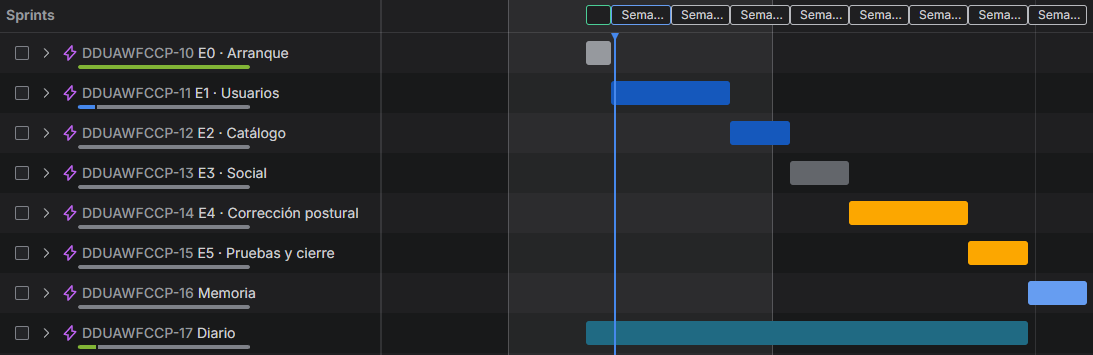
\includegraphics[width=\textwidth]{img/jira-cronograma.png}
        \caption{Cronograma del proyecto en Jira, con las épicas y su planificación temporal.}
        \label{fig:jira-cronograma}
    \end{figure}
    
    Para clasificar el trabajo de forma transversal a las épicas se emplea un
    sistema de \textit{etiquetas} según el área técnica de cada tarea:
    \texttt{setup}, \texttt{infra}, \texttt{backend}, \texttt{frontend},
    \texttt{data}, \texttt{postural}, \texttt{design}, \texttt{testing} y
    \texttt{memoria}. Esto facilita filtrar y consultar el trabajo por tipo de
    actividad con independencia del sprint en que se realice.
    
    Por último, se definen dos épicas de apoyo. La épica \textit{Hitos} recoge
    las fechas de vencimiento clave del proyecto (aplicación funcionalmente
    completa, entrega de la memoria al tutor, solicitud de defensa y defensa),
    que actúan como puntos de control fijos. La épica \textit{Diario} materializa
    la estrategia de documentación incremental: cada entrada registra una
    decisión, un resultado o una incidencia y se anota con el capítulo de la
    memoria al que alimenta, de modo que la memoria crece en paralelo al
    desarrollo en lugar de redactarse íntegramente al final.


    \section{Estructura de la memoria}
    
    El resto de la memoria se organiza como sigue. El Capítulo~\ref{cap:estado-del-arte}
    revisa el estado del arte en aplicaciones de fitness y corrección postural.
    El Capítulo~\ref{cap:tecnologias} describe las tecnologías y herramientas
    empleadas. El Capítulo~\ref{cap:analisis} recoge el análisis de
    requisitos. El Capítulo~\ref{cap:diseno} detalla el diseño del sistema. El
    Capítulo~\ref{cap:implementacion} aborda la implementación. El
    Capítulo~\ref{cap:pruebas} presenta las pruebas y la validación. Finalmente,
    el Capítulo~\ref{cap:conclusiones} expone las conclusiones y las líneas de
    trabajo futuro.


% ─────────────────────── Capítulo 2 ──────────────────────────────────


    \chapter{Estado del arte}
    \label{cap:estado-del-arte}

    \section{Aplicaciones de fitness actuales}
    
    El mercado de aplicaciones de fitness ha crecido de forma sostenida en los
    últimos años, ofreciendo rutinas de entrenamiento, catálogos de ejercicios
    y herramientas de seguimiento de la actividad. Sin embargo, la mayoría de
    estas soluciones se limitan a presentar contenido estático o guías
    visuales, y no proporcionan mecanismos objetivos para evaluar o corregir la
    técnica de ejecución del usuario.
    
    \section{Estimación de pose y corrección postural}
    
    % AMPLIAR: esta sección necesita fuentes propias. Explica brevemente qué es
    % la estimación de pose por visión por computador, menciona MediaPipe Pose
    % y cita 2-3 trabajos o herramientas similares.
    
    Las técnicas de estimación de pose permiten detectar puntos clave del
    cuerpo humano a partir de imágenes o vídeo y calcular métricas como ángulos
    articulares y alineaciones. Herramientas como MediaPipe Pose posibilitan
    realizar este análisis en tiempo real y directamente en el navegador, sin
    necesidad de equipamiento especializado.
    
    \section{Aportación diferencial del proyecto}
    
    A diferencia de las soluciones existentes, centradas en el consumo de
    contenido o en el registro del entrenamiento, este proyecto integra el
    análisis postural como un elemento central del sistema, manteniendo un
    alcance realista acorde a un Trabajo Fin de Grado. El objetivo no es
    sustituir a un entrenador profesional, sino ofrecer una herramienta de
    apoyo que ayude a reducir errores comunes en el entrenamiento autónomo.


% ─────────────────────── Capítulo 3 ──────────────────────────────────


    \chapter{Tecnologías y herramientas}
    \label{cap:tecnologias}
    
    Este capítulo describe las tecnologías y herramientas empleadas en el
    desarrollo del proyecto, así como las versiones concretas utilizadas, que se
    recogen en la Tabla~\ref{tab:versiones}.
    
    \begin{table}[htbp]
        \centering
        \begin{tabular}{ll}
            \toprule
            \textbf{Herramienta} & \textbf{Versión} \\
            \midrule
            Node.js        & 24.18.0 \\
            npm            & 12.0.1 \\
            Angular CLI    & 22.0.6 \\
            Java (JDK)     & 21 \\
            Spring Boot    & 4.1.0 \\
            MySQL          & 8.4 \\
            Docker Desktop & 4.81.0 \\
            Git            & 2.55.0.2 \\
            IntelliJ IDEA  & 2026.1.4 (Ultimate) \\
            Postman        & 12.19.0 \\
            jjwt (JWT)     & 0.13.0 \\
            Figma          & Web \\
            \bottomrule
        \end{tabular}
        \caption{Versiones de las principales tecnologías y herramientas.}
        \label{tab:versiones}
    \end{table}
    
    \section{Frontend: Angular, NgRx y SCSS}
    
    La interfaz de usuario se desarrolla con Angular, un framework de código
    abierto para la construcción de aplicaciones web de página única (SPA)
    basado en TypeScript. La gestión del estado de la aplicación se realiza con
    NgRx, una librería que implementa el patrón Redux y centraliza el estado en
    un único almacén, facilitando su trazabilidad. Para los estilos se emplea
    SCSS, una extensión de CSS que aporta variables y anidamiento, y el formato
    del código se mantiene consistente mediante la herramienta Prettier.
    
    \section{Backend: Spring Boot, API REST y JWT}
    
    El servidor se implementa con Spring Boot, un framework de Java que agiliza
    la creación de aplicaciones y servicios web. Expone una API REST que
    comunica el frontend con la lógica de negocio mediante peticiones HTTP en
    formato JSON. La seguridad se gestiona con Spring Security y autenticación
    basada en JSON Web Tokens (JWT), que permiten un control de acceso sin
    estado en el servidor. La gestión de dependencias y la construcción del
    proyecto se realizan con Maven, y se emplea Lombok para reducir código
    repetitivo en las clases del modelo. Para probar los endpoints de la API
    de forma aislada durante el desarrollo, sin depender del frontend,
    se ha utilizado Postman, una herramienta para construir y examinar peticiones HTTP.
    
    \section{Persistencia: MySQL y Docker}
    
    La información se almacena en MySQL, un sistema gestor de bases de datos
    relacional. Para facilitar su despliegue y garantizar un entorno
    reproducible, la base de datos se ejecuta en un contenedor Docker con un
    volumen persistente, de modo que los datos se conservan entre reinicios sin
    necesidad de instalar MySQL directamente en el sistema anfitrión.
    
    \section{Visión por computador: MediaPipe Pose}
    
    El módulo de corrección postural se apoya en MediaPipe Pose, concretamente
    en el modelo PoseLandmarker, que permite detectar los puntos clave del
    cuerpo humano a partir de vídeo. El procesamiento se realiza directamente en
    el navegador mediante WebAssembly (WASM), lo que evita enviar y almacenar
    los vídeos del usuario y preserva su privacidad. A partir de los puntos
    detectados se calculan métricas como ángulos articulares y alineaciones.
    
    \section{Entorno de desarrollo, control de versiones y gestión de tareas}
    
    El desarrollo se lleva a cabo en el IDE IntelliJ IDEA. El control de
    versiones se gestiona con Git, utilizando GitHub como repositorio remoto,
    organizado como un monorepo que agrupa el frontend, el backend y la
    documentación en un único proyecto. La planificación y el seguimiento de las
    tareas se realizan con Jira, tal como se describe en la
    Sección~\ref{subsec:metodologia} (metodología y gestión del proyecto).

    El diseño de la interfaz se ha elaborado previamente con Figma, una
    herramienta de diseño y prototipado que permite definir un sistema de
    diseño (paleta, tipografía y componentes) y construir maquetas de alta
    fidelidad de cada pantalla antes de su implementación. Su uso ha permitido
    validar la disposición de los elementos y los flujos de navegación antes de
    escribir código, reduciendo el retrabajo durante el desarrollo.


% ─────────────────────── Capítulo 4 ──────────────────────────────────


    \chapter{Análisis de requisitos}
    \label{cap:analisis}


    
    \section{Requisitos funcionales}
    En esta sección se recogen los requisitos funcionales del sistema, es decir,
    las funcionalidades que debe ofrecer la aplicación. La
    Tabla~\ref{tab:req-funcionales} los enumera.
    
    \begin{table}[htbp]
        \centering
        \begin{tabular}{l p{10cm}}
            \toprule
            \textbf{ID} & \textbf{Descripción} \\
            \midrule
            RF-01 & El usuario podrá registrarse, iniciar y cerrar sesión de forma segura. \\
            RF-02 & El usuario autenticado podrá consultar un catálogo de ejercicios. \\
            RF-03 & El usuario podrá filtrar los ejercicios por nombre, grupo muscular y nivel de dificultad. \\
            RF-04 & El usuario podrá ver el detalle de un ejercicio, con descripción, consejos y vídeo embebido. \\
            RF-05 & El usuario podrá valorar los ejercicios mediante un sistema de estrellas, y consultar la valoración media de cada ejercicio junto con la distribución de las puntuaciones recibidas. \\
            RF-06 & El usuario podrá escribir, editar y eliminar un comentario propio sobre un ejercicio, así como consultar los comentarios de los demás usuarios. \\
            RF-07 & El usuario podrá marcar ejercicios como favoritos y consultarlos en un listado propio, con las mismas opciones de búsqueda y filtrado que el catálogo. \\
            RF-08 & El usuario podrá subir un vídeo local para analizar su ejecución postural. \\
            RF-09 & El sistema calculará métricas (ángulos y alineaciones) a partir del vídeo. \\
            RF-10 & El sistema mostrará una puntuación global y recomendaciones de corrección. \\
            RF-11 & El usuario podrá consultar el historial de sus análisis posturales anteriores. \\
            \bottomrule
        \end{tabular}
        \caption{Requisitos funcionales del sistema.}
        \label{tab:req-funcionales},
    \end{table}

    Conviene precisar el alcance del requisito RF-11 en relación con el
    RNF-02. El historial almacena únicamente el resultado del análisis la
    puntuación obtenida, el ejercicio evaluado y la fecha, nunca el vídeo
    empleado, que se procesa en el navegador y no se transmite en ningún
    momento al servidor. Ambos requisitos son, por tanto, compatibles.
    
    \section{Requisitos no funcionales}

    Los requisitos no funcionales establecen las condiciones y restricciones de
    calidad que debe cumplir el sistema, como la seguridad, la privacidad o la
    usabilidad, más allá de sus funcionalidades concretas. La
    Tabla~\ref{tab:req-no-funcionales} los recoge.
    
    \begin{table}[htbp]
        \centering
        \begin{tabular}{l p{10cm}}
            \toprule
            \textbf{ID} & \textbf{Descripción} \\
            \midrule
            RNF-01 & Las contraseñas se almacenarán cifradas y el acceso a los recursos protegidos se controlará mediante JWT. \\
            RNF-02 & El procesamiento de los vídeos se realizará en el navegador, sin almacenar contenido del usuario, preservando su privacidad. \\
            RNF-03 & La interfaz será usable e intuitiva, con una navegación clara entre las distintas vistas. \\
            RNF-04 & El sistema seguirá una arquitectura cliente-servidor desacoplada mediante una API REST. \\
            RNF-05 & La aplicación será desplegable de forma reproducible mediante contenedores. \\
            RNF-06 & La aplicación funcionará en navegadores web modernos (Chrome, Firefox). \\
            \bottomrule
        \end{tabular}
        \caption{Requisitos no funcionales del sistema.}
        \label{tab:req-no-funcionales}
    \end{table}

    \section{Reglas de negocio}

    Más allá de las funcionalidades ofrecidas, el sistema debe hacer cumplir un
    conjunto de restricciones sobre los datos que no se deducen del enunciado
    de los requisitos y que condicionan tanto el modelo de datos como el diseño
    de la API. La Tabla~\ref{tab:reglas-negocio} las recoge.

    \begin{table}[htbp]
        \centering
        \begin{tabular}{l p{10cm}}
            \toprule
            \textbf{ID} & \textbf{Descripción} \\
            \midrule
            RN-01 & Cada usuario puede emitir como máximo una valoración por ejercicio. Publicar de nuevo sustituye a la anterior. \\
            RN-02 & La puntuación es obligatoria y toma un valor entero entre 1 y 5. \\
            RN-03 & El comentario es opcional: un usuario puede puntuar un ejercicio sin escribir texto alguno. \\
            RN-04 & Un usuario solo puede modificar o eliminar su propia valoración. \\
            RN-05 & Un ejercicio puede figurar entre los favoritos de un usuario una sola vez. \\
            RN-06 & La valoración media de un ejercicio se calcula a partir de las valoraciones existentes y no se almacena de forma redundante. \\
            \bottomrule
        \end{tabular}
        \caption{Reglas de negocio del módulo de valoraciones y favoritos.}
        \label{tab:reglas-negocio}
    \end{table}

    Estas reglas se aplican en distintos puntos del sistema y con distinto
    grado de garantía. Las que expresan una restricción estructural (RN-01 y
    RN-05) se imponen en la propia base de datos mediante restricciones de
    unicidad, y no únicamente mediante comprobaciones en el código; las que
    acotan un valor (RN-02 y RN-03) se validan sobre los datos de entrada de la
    API; y RN-04 se garantiza por diseño, al no existir ninguna operación que
    permita referirse a la valoración de otro usuario. Los mecanismos concretos
    se detallan en el Capítulo~\ref{cap:implementacion}.
    
    \section{Actores del sistema}

    El sistema contempla dos actores. El \textbf{visitante} es quien accede a
    la aplicación sin haberse identificado; su interacción se limita a la
    página de presentación, el registro y el inicio de sesión. El
    \textbf{usuario registrado} es quien ha iniciado sesión y dispone de acceso
    a la totalidad de las funcionalidades: consulta del catálogo, valoración de
    ejercicios, gestión de favoritos y análisis postural.

    El modelo de datos contempla además un rol de administrador, previsto para
    la gestión del catálogo, que no se ha desarrollado como actor del sistema
    por quedar fuera del alcance de este trabajo: el catálogo se carga de forma
    programada al arrancar la aplicación, según se describe en el
    Capítulo~\ref{cap:implementacion}.

    \section{Casos de uso}

    La Tabla~\ref{tab:casos-uso} recoge los casos de uso identificados, junto
    con el actor que los inicia y el requisito funcional del que derivan.

    \begin{table}[htbp]
        \centering
        \small
        \begin{tabular}{l p{6.5cm} l l}
            \toprule
            \textbf{ID} & \textbf{Caso de uso} & \textbf{Actor} & \textbf{Req.} \\
            \midrule
            CU-01 & Registrarse en la aplicación            & Visitante & RF-01 \\
            CU-02 & Iniciar sesión                          & Visitante & RF-01 \\
            CU-03 & Cerrar sesión                           & Usuario   & RF-01 \\
            CU-04 & Consultar y modificar el perfil propio  & Usuario   & RF-01 \\
            CU-05 & Consultar el catálogo de ejercicios     & Usuario   & RF-02 \\
            CU-06 & Buscar y filtrar ejercicios             & Usuario   & RF-03 \\
            CU-07 & Consultar el detalle de un ejercicio    & Usuario   & RF-04 \\
            CU-08 & Valorar un ejercicio                    & Usuario   & RF-05 \\
            CU-09 & Comentar un ejercicio                   & Usuario   & RF-06 \\
            CU-10 & Consultar las valoraciones de un ejercicio & Usuario & RF-05, RF-06 \\
            CU-11 & Marcar y desmarcar un ejercicio como favorito & Usuario & RF-07 \\
            CU-12 & Consultar los ejercicios favoritos      & Usuario   & RF-07 \\
            CU-13 & Analizar la técnica de ejecución        & Usuario   & RF-08 \\
            \bottomrule
        \end{tabular}
        \caption{Casos de uso del sistema.}
        \label{tab:casos-uso}
    \end{table}

    La Figura~\ref{fig:casos-uso} representa gráficamente estos casos y su
    relación con los actores.

    \begin{figure}[htbp]
        \centering
        \begin{tikzpicture}[
            font=\footnotesize,
            uc/.style={draw, ellipse, align=center, minimum width=64mm,
                       minimum height=8mm, inner sep=2pt, text width=54mm},
            rel/.style={draw, thin}
        ]

        % ─── Límite del sistema ───
        \draw[rounded corners=3pt] (0.3, 0.95) rectangle (8.7, -13.9);
        \node[font=\small\bfseries] at (4.5, 0.45) {PoseCoach};

        % ─── Casos de uso ───
        \node[uc] (cu01) at (4.5,  -0.50) {CU-01 · Registrarse en la aplicación};
        \node[uc] (cu02) at (4.5,  -1.55) {CU-02 · Iniciar sesión};
        \node[uc] (cu03) at (4.5,  -2.60) {CU-03 · Cerrar sesión};
        \node[uc] (cu04) at (4.5,  -3.65) {CU-04 · Consultar y modificar el perfil propio};
        \node[uc] (cu05) at (4.5,  -4.70) {CU-05 · Consultar el catálogo de ejercicios};
        \node[uc] (cu06) at (4.5,  -5.75) {CU-06 · Buscar y filtrar ejercicios};
        \node[uc] (cu07) at (4.5,  -6.80) {CU-07 · Consultar el detalle de un ejercicio};
        \node[uc] (cu08) at (4.5,  -7.85) {CU-08 · Valorar un ejercicio};
        \node[uc] (cu09) at (4.5,  -8.90) {CU-09 · Comentar un ejercicio};
        \node[uc] (cu10) at (4.5,  -9.95) {CU-10 · Consultar las valoraciones de un ejercicio};
        \node[uc] (cu11) at (4.5, -11.00) {CU-11 · Marcar y desmarcar un ejercicio como favorito};
        \node[uc] (cu12) at (4.5, -12.05) {CU-12 · Consultar los ejercicios favoritos};
        \node[uc] (cu13) at (4.5, -13.10) {CU-13 · Analizar la técnica de ejecución};

        % ─── Actor: visitante ───
        \begin{scope}[shift={(-2.6,-1.00)}]
            \draw (0, 0.60) circle (0.17);
            \draw (0, 0.43) -- (0,-0.05);
            \draw (-0.27, 0.27) -- (0.27, 0.27);
            \draw (0,-0.05) -- (-0.21,-0.44);
            \draw (0,-0.05) -- ( 0.21,-0.44);
            \node[align=center, font=\footnotesize\bfseries] at (0,-0.80) {Visitante};
        \end{scope}
        \coordinate (av) at (-2.05,-1.00);

        % ─── Actor: usuario registrado ───
        \begin{scope}[shift={(-2.6,-7.85)}]
            \draw (0, 0.60) circle (0.17);
            \draw (0, 0.43) -- (0,-0.05);
            \draw (-0.27, 0.27) -- (0.27, 0.27);
            \draw (0,-0.05) -- (-0.21,-0.44);
            \draw (0,-0.05) -- ( 0.21,-0.44);
            \node[align=center, font=\footnotesize\bfseries] at (0,-0.90)
                 {Usuario\\registrado};
        \end{scope}
        \coordinate (au) at (-2.05,-7.85);

        % ─── Asociaciones del visitante ───
        \draw[rel] (av) -- (cu01.west);
        \draw[rel] (av) -- (cu02.west);

        % ─── Asociaciones del usuario registrado ───
        \foreach \c in {cu03,cu04,cu05,cu06,cu07,cu08,cu09,cu10,cu11,cu12,cu13}
            \draw[rel] (au) -- (\c.west);

        \end{tikzpicture}
        \caption{Diagrama de casos de uso del sistema.}
        \label{fig:casos-uso}
    \end{figure}

    A continuación se detallan tres de los casos de uso, seleccionados por
    concentrar las decisiones de diseño y las reglas de negocio más relevantes
    del sistema.

    \begin{table}[htbp]
        \centering
        \small
        \begin{tabular}{p{2.7cm} p{9.8cm}}
            \toprule
            \multicolumn{2}{l}{\textbf{CU-06 · Buscar y filtrar ejercicios}} \\
            \midrule
            Actor & Usuario registrado \\
            Descripción & El usuario acota el catálogo mediante una búsqueda por nombre y una combinación de filtros por grupo muscular y dificultad. \\
            Precondición & El usuario ha iniciado sesión y se encuentra en el catálogo. \\
            Flujo principal & 1. El usuario introduce un texto de búsqueda, selecciona uno o varios grupos musculares o elige un nivel de dificultad. \newline
                              2. El sistema recupera los ejercicios que satisfacen todos los criterios indicados. \newline
                              3. El sistema muestra los resultados junto con su número total. \\
            Flujo alternativo A & Si se seleccionan varios grupos musculares, el sistema incluye los ejercicios que trabajen alguno de ellos, no necesariamente todos. \\
            Flujo alternativo B & Si ninguna combinación arroja resultados, el sistema lo indica y ofrece deshacer los filtros, distinguiendo esta situación de un catálogo vacío. \\
            Postcondición & El listado refleja los criterios activos, que quedan reflejados en la dirección de la vista. \\
            \bottomrule
        \end{tabular}
        \caption{Descripción detallada del caso de uso CU-06.}
        \label{tab:cu-06}
    \end{table}

    \begin{table}[htbp]
        \centering
        \small
        \begin{tabular}{p{2.7cm} p{9.8cm}}
            \toprule
            \multicolumn{2}{l}{\textbf{CU-08 · Valorar un ejercicio}} \\
            \midrule
            Actor & Usuario registrado \\
            Descripción & El usuario asigna una puntuación de 1 a 5 estrellas a un ejercicio, opcionalmente acompañada de un comentario. \\
            Precondición & El usuario ha iniciado sesión y consulta el detalle de un ejercicio existente. \\
            Flujo principal & 1. El usuario abre la pestaña de valoraciones. \newline
                              2. El sistema muestra la media, la distribución de puntuaciones y los comentarios existentes. \newline
                              3. El usuario selecciona una puntuación y, si lo desea, redacta un comentario. \newline
                              4. El usuario confirma la publicación. \newline
                              5. El sistema registra la valoración y actualiza la media, la distribución y el listado. \\
            Flujo alternativo A & Si el usuario ya había valorado el ejercicio, la nueva valoración sustituye a la anterior (RN-01). \\
            Flujo alternativo B & Si el usuario no selecciona puntuación, el sistema impide la publicación (RN-02). \\
            Flujo alternativo C & Si el usuario no redacta comentario, la valoración se registra igualmente y computa en la media, sin figurar en el listado de comentarios (RN-03). \\
            Postcondición & El ejercicio cuenta con exactamente una valoración del usuario. \\
            \bottomrule
        \end{tabular}
        \caption{Descripción detallada del caso de uso CU-08.}
        \label{tab:cu-08}
    \end{table}

    \begin{table}[htbp]
        \centering
        \small
        \begin{tabular}{p{2.7cm} p{9.8cm}}
            \toprule
            \multicolumn{2}{l}{\textbf{CU-11 · Marcar y desmarcar un ejercicio como favorito}} \\
            \midrule
            Actor & Usuario registrado \\
            Descripción & El usuario añade un ejercicio a su lista personal de favoritos, o lo retira de ella. \\
            Precondición & El usuario ha iniciado sesión y visualiza el ejercicio, ya sea en el catálogo, en su detalle o en la lista de favoritos. \\
            Flujo principal & 1. El usuario acciona el control de favorito del ejercicio. \newline
                              2. El sistema refleja de inmediato el nuevo estado en la interfaz. \newline
                              3. El sistema registra el cambio de forma permanente. \\
            Flujo alternativo A & Si la operación no llega a registrarse, el sistema restablece el estado anterior en la interfaz. \\
            Flujo alternativo B & Si se solicita un estado que ya se cumple, la operación se completa sin efecto ni error (RN-05). \\
            Flujo alternativo C & Si la acción se realiza desde la lista de favoritos, el ejercicio desaparece de ella al desmarcarse. \\
            Postcondición & El ejercicio figura o deja de figurar entre los favoritos del usuario, de forma coherente en todas las vistas. \\
            \bottomrule
        \end{tabular}
        \caption{Descripción detallada del caso de uso CU-11.}
        \label{tab:cu-11}
    \end{table}


% ─────────────────────── Capítulo 5 ──────────────────────────────────


    \chapter{Diseño del sistema}
    \label{cap:diseno}


    \section{Arquitectura general (cliente-servidor)}
    El sistema sigue una arquitectura cliente-servidor de tres capas. El
    cliente es una aplicación web desarrollada en Angular que se ejecuta en el
    navegador, el servidor es una API REST implementada con Spring Boot, y la
    persistencia se delega en una base de datos MySQL. La comunicación entre
    cliente y servidor se realiza mediante peticiones HTTP con formato JSON,
    mientras que el servidor accede a la base de datos mediante consultas SQL.
    La Figura~\ref{fig:arquitectura-general} muestra esta organización.

    \begin{figure}[htbp]
        \centering
        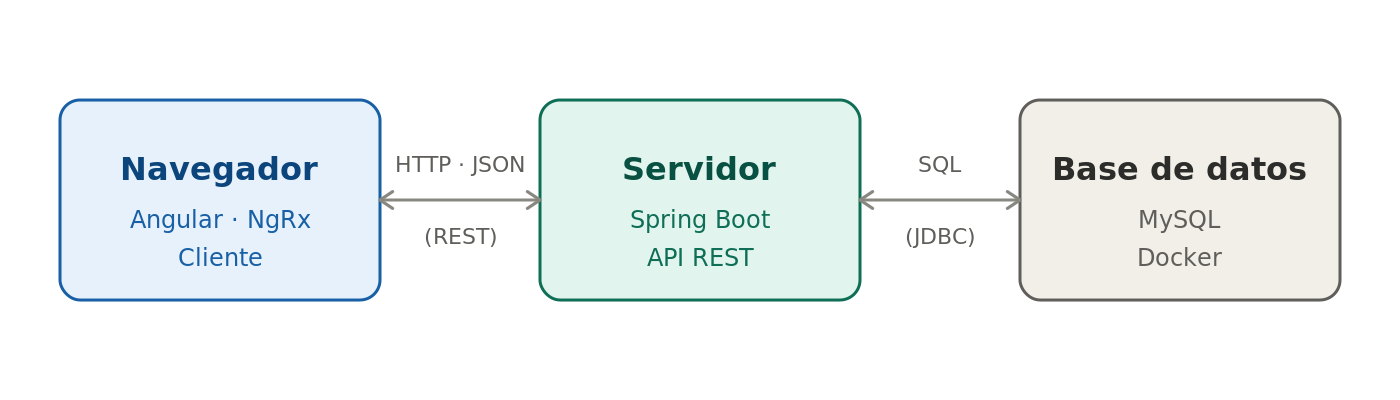
\includegraphics[width=0.9\textwidth]{img/arquitectura-general.png}
        \caption{Arquitectura general del sistema.}
        \label{fig:arquitectura-general}
    \end{figure}


    \section{Modelo de datos}

    El modelo de datos parte de la entidad central \texttt{User}, que
    almacena la información necesaria para la autenticación y el perfil del
    usuario. La contraseña nunca se guarda en texto plano, sino cifrada
    mediante el algoritmo BCrypt. La Tabla~\ref{tab:entidad-user} recoge sus
    atributos.

    \begin{table}[htbp]
        \centering
        \begin{tabular}{lll}
            \toprule
            \textbf{Atributo} & \textbf{Tipo} & \textbf{Descripción} \\
            \midrule
            id        & Long          & Identificador único (clave primaria) \\
            username  & String        & Nombre de usuario, único \\
            email     & String        & Correo electrónico, único \\
            password  & String        & Contraseña cifrada (BCrypt) \\
            role      & Enum          & Rol: USER o ADMIN \\
            createdAt & LocalDateTime & Fecha de alta \\
        \bottomrule
        \end{tabular}
        \caption{Atributos de la entidad \texttt{User}.}
        \label{tab:entidad-user}
    \end{table}

    La segunda entidad del modelo es \texttt{Exercise}, que representa cada
    uno de los ejercicios del catálogo. Sus atributos se recogen en la
    Tabla~\ref{tab:entidad-exercise}.

    \begin{table}[htbp]
        \centering
        \begin{tabular}{lll}
            \toprule
            \textbf{Atributo} & \textbf{Tipo} & \textbf{Descripción} \\
            \midrule
            id             & Long             & Identificador único (clave primaria) \\
            name           & String           & Nombre del ejercicio, único \\
            description    & String           & Descripción del movimiento \\
            muscleGroups   & Conjunto de Enum & Grupos musculares implicados \\
            difficulty     & Enum             & Nivel de dificultad \\
            youtubeVideoId & String           & Identificador del vídeo en YouTube \\
            tips           & Lista de String  & Consejos de ejecución, ordenados \\
            analysisType   & Enum             & Analizador postural asociado (opcional) \\
            createdAt      & LocalDateTime    & Fecha de alta \\
            \bottomrule
        \end{tabular}
        \caption{Atributos de la entidad \texttt{Exercise}.}
        \label{tab:entidad-exercise}
    \end{table}

    Tres de estos atributos requieren una justificación explícita, ya que
    condicionan tanto el esquema relacional como el diseño de la API.

    En primer lugar, un mismo ejercicio implica habitualmente más de un grupo
    muscular: las dominadas trabajan espalda y brazos, y la sentadilla, pierna
    y glúteo. Por ello \texttt{muscleGroups} no es un valor simple sino un
    conjunto. Se descartó modelar el grupo muscular como una entidad propia
    porque se trata de un conjunto cerrado de valores sin atributos asociados,
    para el que un tipo enumerado resulta suficiente y evita una tabla y una
    relación adicionales. Lo mismo ocurre con los consejos de ejecución
    (\texttt{tips}), que son textos sin identidad propia y carecen de sentido
    fuera del ejercicio al que pertenecen. Ambos se mapean como colecciones de
    elementos, lo que da lugar a las tres tablas físicas recogidas en la
    Tabla~\ref{tab:tablas-catalogo}.

    \begin{table}[htbp]
        \centering
        \begin{tabular}{ll}
            \toprule
            \textbf{Tabla} & \textbf{Contenido} \\
            \midrule
            exercises              & Atributos simples del ejercicio \\
            exercise\_muscle\_groups & Grupos musculares de cada ejercicio \\
            exercise\_tips           & Consejos de cada ejercicio, con su orden \\
            \bottomrule
        \end{tabular}
        \caption{Tablas que componen el catálogo de ejercicios.}
        \label{tab:tablas-catalogo}
    \end{table}

    En segundo lugar, del vídeo demostrativo se almacena únicamente el
    identificador que YouTube asigna a cada contenido, y no su dirección
    completa. A partir de ese identificador el cliente compone tanto la
    dirección de reproducción embebida como la de la miniatura, sin necesidad
    de analizar cadenas de texto. Esta decisión tiene además una consecuencia
    relevante en materia de derechos de autor: la imagen que ilustra cada
    ejercicio es la miniatura servida por la propia plataforma junto al enlace
    al vídeo original, lo que evita incorporar a la memoria y al repositorio
    ilustraciones anatómicas de terceros, algo especialmente pertinente dado
    que este trabajo se publica en el repositorio institucional RIUMA.

    En tercer lugar, el atributo \texttt{analysisType} indica qué analizador
    postural corresponde a cada ejercicio y admite valor nulo. Los ejercicios
    sin analizador asociado se distinguen así de los analizables, lo que
    permite a la interfaz mostrar u ocultar el acceso al módulo de corrección
    postural. Aunque dicho módulo pertenece a un incremento posterior, el
    atributo se introduce desde el diseño inicial del catálogo para evitar una
    modificación posterior del esquema de la base de datos.

    \subsection{Tipos enumerados del catálogo}

    El catálogo emplea tres tipos enumerados cuyos valores se recogen en la
    Tabla~\ref{tab:enums-catalogo}. Cada valor consta de un identificador
    técnico, que es el que se almacena en la base de datos y viaja en la API,
    y de una etiqueta en castellano, que es la que se muestra al usuario.
    Separar ambos permite modificar el texto visible sin migrar los datos ya
    almacenados y, como se detalla en la Sección~\ref{sec:api-catalogo}, evita
    duplicar las traducciones en el cliente.

    \begin{table}[htbp]
        \centering
        \begin{tabular}{l p{9cm}}
            \toprule
            \textbf{Tipo} & \textbf{Valores} \\
            \midrule
            MuscleGroup  & Pecho, Espalda, Hombros, Brazos, Pierna, Glúteo,
                           Abdominales y Oblicuos \\
            Difficulty   & Fácil, Medio y Difícil \\
            AnalysisType & Sentadilla, Zancada, Plancha y Flexión \\
            \bottomrule
        \end{tabular}
        \caption{Tipos enumerados empleados en el catálogo de ejercicios.}
        \label{tab:enums-catalogo}
    \end{table}

    La lista de grupos musculares es deliberadamente cerrada y de granularidad
    media. Una clasificación anatómica exhaustiva habría resultado excesiva
    para el propósito de la aplicación, que es permitir al usuario localizar
    ejercicios por zona de trabajo, no ofrecer una referencia anatómica.

    \subsection{Valoraciones y favoritos}

    El módulo social introduce dos entidades que relacionan usuarios con
    ejercicios. La primera, \texttt{Review}, recoge la valoración que un
    usuario emite sobre un ejercicio; la segunda, \texttt{Favorite}, registra
    los ejercicios que un usuario ha marcado para tenerlos localizados. Sus
    atributos se detallan en las Tablas~\ref{tab:entidad-review}
    y~\ref{tab:entidad-favorite}.

    \begin{table}[htbp]
        \centering
        \begin{tabular}{lll}
            \toprule
            \textbf{Atributo} & \textbf{Tipo} & \textbf{Descripción} \\
            \midrule
            id        & Long          & Identificador único (clave primaria) \\
            user      & User          & Autor de la valoración \\
            exercise  & Exercise      & Ejercicio valorado \\
            score     & int           & Puntuación de 1 a 5 \\
            content   & String        & Comentario, opcional (máx. 500 caracteres) \\
            createdAt & LocalDateTime & Fecha de publicación \\
            updatedAt & LocalDateTime & Fecha de la última modificación \\
            \bottomrule
        \end{tabular}
        \caption{Atributos de la entidad \texttt{Review}.}
        \label{tab:entidad-review}
    \end{table}

    \begin{table}[htbp]
        \centering
        \begin{tabular}{lll}
            \toprule
            \textbf{Atributo} & \textbf{Tipo} & \textbf{Descripción} \\
            \midrule
            id        & Long          & Identificador único (clave primaria) \\
            user      & User          & Usuario que marca el favorito \\
            exercise  & Exercise      & Ejercicio marcado \\
            createdAt & LocalDateTime & Fecha en que se marcó \\
            \bottomrule
        \end{tabular}
        \caption{Atributos de la entidad \texttt{Favorite}.}
        \label{tab:entidad-favorite}
    \end{table}

    La decisión de diseño más relevante de este modelo es que los requisitos
    RF-05 y RF-06, que el enunciado presenta como funcionalidades separadas, se
    satisfacen con \textbf{una única entidad}. El motivo procede del diseño de
    la interfaz: la puntuación y el comentario se publican mediante un solo
    formulario y una sola acción, y cada comentario se muestra siempre
    acompañado de las estrellas de su autor. Modelarlos por separado habría
    obligado a reconstruir mediante una reunión de tablas algo que el usuario
    percibe como un único objeto, y habría permitido estados incoherentes, como
    un comentario sin puntuación asociada.

    De esa unificación se deriva que el atributo \texttt{content} admita valor
    nulo. Un usuario puede puntuar sin escribir nada, situación habitual y
    prevista por la interfaz, en cuyo caso la valoración computa en la media y
    en la distribución pero no aparece en el listado de comentarios. Esto
    explica que el número de valoraciones de un ejercicio sea siempre mayor o
    igual que el de comentarios, sin que ello suponga ninguna inconsistencia.

    Ambas entidades incorporan una restricción de unicidad sobre el par
    (usuario, ejercicio), que es el mecanismo que hace cumplir las reglas RN-01
    y RN-05. Situar esta garantía en la base de datos, y no solo en la lógica
    de la aplicación, resulta necesario porque dos peticiones simultáneas del
    mismo usuario podrían superar ambas una comprobación previa en el código y
    generar filas duplicadas; la restricción de la tabla rechaza la segunda en
    cualquier caso. Es el mismo criterio aplicado a los campos
    \texttt{username} y \texttt{email} de la entidad \texttt{User}.

    La entidad \texttt{Review} registra dos marcas temporales porque la
    valoración es modificable. Al sustituirse el contenido de la fila, la fecha
    de creación deja de describir el estado actual del dato, de modo que
    \texttt{updatedAt} recoge cuándo se fijó el valor vigente. La interfaz
    aprovecha ambas: ordena los comentarios por fecha de publicación, para que
    una corrección menor no altere su posición en la lista, y señala como
    editados aquellos en los que ambas fechas difieren.

    Merece justificación aparte que \texttt{Favorite} se haya modelado como una
    entidad y no como una relación de muchos a muchos entre \texttt{User} y
    \texttt{Exercise}, que es la construcción que JPA ofrece de forma directa
    para este caso. El motivo es que la relación posee un atributo propio: la
    fecha en que se marcó el favorito, que determina el orden del listado. Una
    relación de muchos a muchos genera una tabla intermedia capaz de albergar
    únicamente las dos claves ajenas, por lo que ese dato no tendría dónde
    almacenarse. En el momento en que una relación incorpora información
    propia, deja de ser una relación y pasa a ser una entidad.

    Por último, y conforme a la regla RN-06, la valoración media no figura como
    atributo de \texttt{Exercise}. Almacenarla habría permitido consultarla sin
    cálculo alguno, pero introduce un dato redundante que debe mantenerse
    sincronizado con cada alta, modificación y baja de valoración, y que queda
    incorrecto en cuanto una de esas actualizaciones falla. Se ha optado por
    calcularla en cada consulta; el Capítulo~\ref{cap:implementacion} detalla
    cómo se hace sin penalizar el rendimiento del listado.

    La Figura~\ref{fig:modelo-datos} resume el modelo de datos completo, con
    las cinco entidades del sistema y las relaciones entre ellas.

    \begin{figure}[htbp]
        \centering
        \includegraphics[width=\textwidth]{img/modelo-datos.png}
        \caption{Modelo de datos del sistema, con las entidades del catálogo,
        de usuarios y del módulo social.}
        \label{fig:modelo-datos}
    \end{figure}


    \section{Diseño de la API REST}
    La comunicación entre cliente y servidor se realiza mediante una API REST
    que intercambia mensajes en formato JSON sobre HTTP. Cada operación se asocia
    a una ruta y a un verbo HTTP, y la respuesta se acompaña del código de estado
    HTTP correspondiente al resultado. El módulo de autenticación expone las
    rutas recogidas en la Tabla~\ref{tab:api-auth}, ambas públicas por no
    requerir un usuario autenticado previo.

    \begin{table}[htbp]
        \centering
        \begin{tabular}{lll}
            \toprule
            \textbf{Verbo} & \textbf{Ruta} & \textbf{Descripción} \\
            \midrule
            POST & /api/auth/register & Registro de un nuevo usuario \\
            POST & /api/auth/login    & Inicio de sesión y obtención del token \\
            GET & /api/users/me & Consultar el perfil del usuario autenticado \\
            PUT & /api/users/me & Actualizar el email del usuario autenticado \\
            PUT & /api/users/me/password & Actualizar la contraseña del usuario autenticado \\
            \bottomrule
        \end{tabular}
        \caption{Rutas del módulo de autenticación.}
        \label{tab:api-auth}
    \end{table}

    En el registro, el cuerpo de la petición contiene el nombre de usuario, el
    correo y la contraseña. La respuesta emplea distintos códigos de estado según
    el resultado: \texttt{201 Created} si el usuario se crea correctamente,
    \texttt{400 Bad Request} si los datos no superan la validación (por ejemplo,
    un correo con formato incorrecto) y \texttt{409 Conflict} si el nombre de
    usuario o el correo ya están registrados.

    En el inicio de sesión, el cuerpo de la petición contiene el nombre de
    usuario y la contraseña. Si las credenciales son correctas, la respuesta es
    \texttt{200 OK} e incluye el token JWT que el cliente deberá presentar en
    las peticiones posteriores; si no lo son, la respuesta es
    \texttt{401 Unauthorized}. Por seguridad, el mensaje de error es idéntico
    tanto si el usuario no existe como si la contraseña es incorrecta, evitando
    así revelar qué nombres de usuario están registrados.

    Una vez autenticado, el usuario dispone además de las rutas recogidas en la
    Tabla~\ref{tab:api-users}, todas ellas privadas: exigen presentar un token
    JWT válido y operan siempre sobre el usuario identificado por dicho token,
    de modo que ningún usuario puede consultar ni modificar los datos de otro.

    \begin{table}[htbp]
        \centering
        \begin{tabular}{lll}
            \toprule
            \textbf{Verbo} & \textbf{Ruta} & \textbf{Descripción} \\
            \midrule
            GET & /api/users/me          & Consulta del perfil propio \\
            PUT & /api/users/me          & Modificación del correo electrónico \\
            PUT & /api/users/me/password & Cambio de contraseña \\
            \bottomrule
        \end{tabular}
        \caption{Rutas del módulo de usuarios.}
        \label{tab:api-users}
    \end{table}

    \subsection{Autenticación basada en tokens (JWT)}

    Para el control de acceso se ha optado por una autenticación basada en
    tokens JWT (\textit{JSON Web Token}) en lugar del modelo clásico de sesiones
    en el servidor. Un JWT es una credencial firmada digitalmente que el
    servidor entrega al usuario tras un inicio de sesión correcto y que este
    presenta en cada petición posterior. El token contiene la información
    necesaria para identificar al usuario (su nombre y su rol) y una fecha de
    caducidad, y va firmado con una clave secreta que solo conoce el servidor,
    lo que le permite verificar su autenticidad sin necesidad de almacenar
    ninguna sesión.

    La principal ventaja de este enfoque es que el servidor es \textit{sin
    estado} (\textit{stateless}): no necesita guardar información de sesión de
    cada usuario, lo que simplifica la arquitectura y facilita la escalabilidad.
    Este modelo encaja además de forma natural con una arquitectura desacoplada
    de frontend y backend que se comunican mediante una API REST, en la que el
    cliente conserva el token y lo adjunta en la cabecera \texttt{Authorization}
    de sus peticiones. Conviene precisar que el token va firmado, pero no
    cifrado, por lo que nunca se incluye en él información sensible como la
    contraseña.

    Conviene subrayar que la protección de rutas en el cliente (mediante un
    \textit{guard} de Angular) cumple únicamente una función de experiencia de
    usuario: evita mostrar vistas privadas cuando no hay sesión. La seguridad
    efectiva reside siempre en el servidor, que revalida el token en cada
    petición con independencia de lo que decida el cliente.

    La Figura~\ref{fig:flujo-auth} resume el flujo completo del módulo de
    autenticación, desde el registro y el inicio de sesión hasta el acceso a una
    ruta protegida presentando el token.

\begin{figure}[htbp]
        \centering
        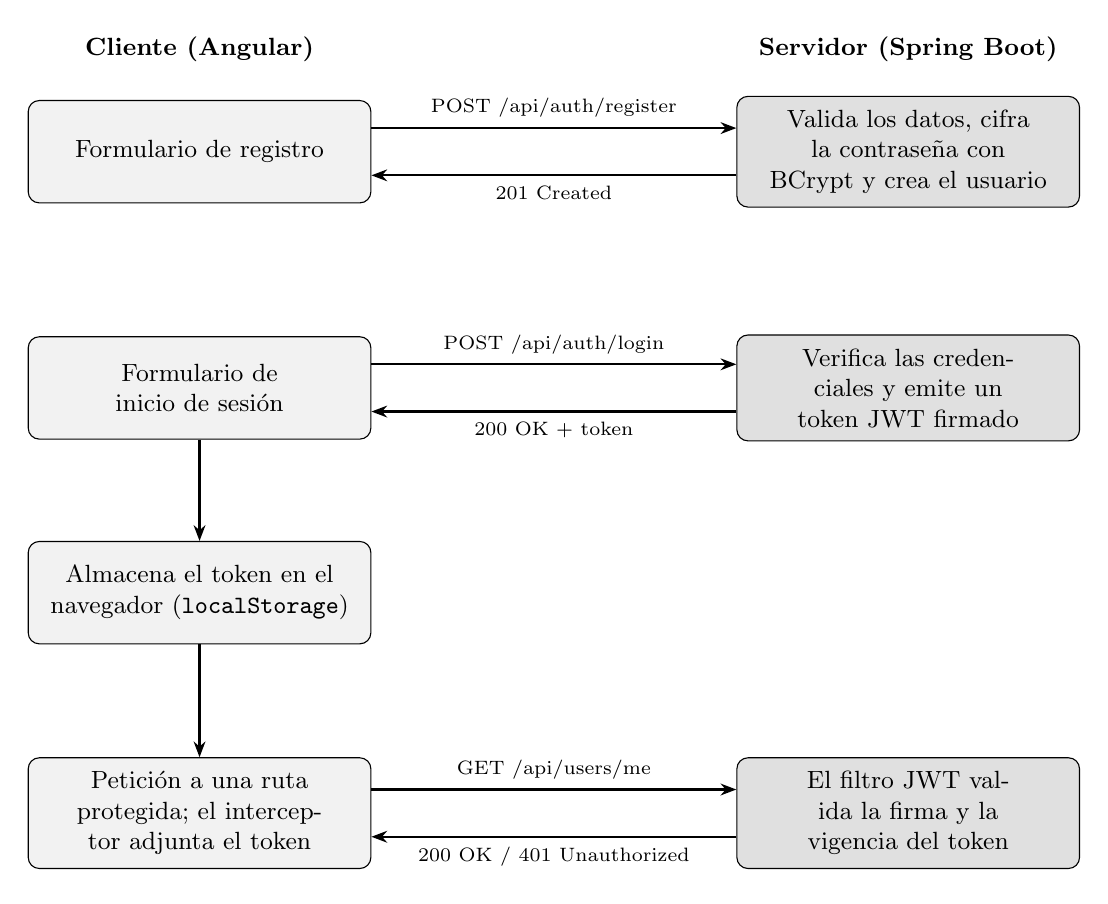
\begin{tikzpicture}[
            font=\small,
            caja/.style={draw, rounded corners, align=center, inner sep=5pt,
                         minimum height=13mm, text width=40mm},
            cliente/.style={caja, fill=black!5},
            servidor/.style={caja, fill=black!12},
            flecha/.style={-{Stealth[length=2mm]}, thick},
            etiq/.style={font=\scriptsize, midway}
        ]

        % Encabezados de columna
        \node[font=\small\bfseries] at (0, 1.3)  {Cliente (Angular)};
        \node[font=\small\bfseries] at (9, 1.3)  {Servidor (Spring Boot)};

        % --- Registro ---
        \node[cliente]  (c1) at (0, 0)    {Formulario de registro};
        \node[servidor] (s1) at (9, 0)    {Valida los datos, cifra la
                                           contraseña con BCrypt y crea
                                           el usuario};
        \draw[flecha] ([yshift=3mm]c1.east) -- ([yshift=3mm]s1.west)
            node[etiq, above] {POST /api/auth/register};
        \draw[flecha] ([yshift=-3mm]s1.west) -- ([yshift=-3mm]c1.east)
            node[etiq, below] {201 Created};

        % --- Inicio de sesión ---
        \node[cliente]  (c2) at (0, -3)   {Formulario de inicio de sesión};
        \node[servidor] (s2) at (9, -3)   {Verifica las credenciales y emite
                                           un token JWT firmado};
        \draw[flecha] ([yshift=3mm]c2.east) -- ([yshift=3mm]s2.west)
            node[etiq, above] {POST /api/auth/login};
        \draw[flecha] ([yshift=-3mm]s2.west) -- ([yshift=-3mm]c2.east)
            node[etiq, below] {200 OK + token};

        % --- Almacenamiento del token ---
        \node[cliente] (c3) at (0, -5.6)  {Almacena el token en el navegador
                                           (\texttt{localStorage})};
        \draw[flecha] (c2) -- (c3);

        % --- Acceso a ruta protegida ---
        \node[cliente]  (c4) at (0, -8.4) {Petición a una ruta protegida;
                                           el interceptor adjunta el token};
        \node[servidor] (s3) at (9, -8.4) {El filtro JWT valida la firma y la
                                           vigencia del token};
        \draw[flecha] (c3) -- (c4);
        \draw[flecha] ([yshift=3mm]c4.east) -- ([yshift=3mm]s3.west)
            node[etiq, above] {GET /api/users/me};
        \draw[flecha] ([yshift=-3mm]s3.west) -- ([yshift=-3mm]c4.east)
            node[etiq, below] {200 OK / 401 Unauthorized};

        \end{tikzpicture}
        \caption{Flujo del módulo de autenticación: registro con cifrado BCrypt,
        inicio de sesión con emisión de token JWT, almacenamiento del token en
        el cliente y acceso a rutas protegidas mediante su validación en el
        servidor.}
        \label{fig:flujo-auth}
    \end{figure}

    \subsection{Catálogo de ejercicios}
    \label{sec:api-catalogo}

    El catálogo expone las tres rutas recogidas en la
    Tabla~\ref{tab:api-catalogo}. A diferencia de las de autenticación, todas
    ellas requieren un usuario autenticado: el acceso al catálogo se ha
    definido como privado porque las tarjetas de ejercicio muestran
    información dependiente del usuario, como su condición de favorito, y
    porque la navegación hacia el catálogo solo está disponible una vez
    iniciada la sesión.

    \begin{table}[htbp]
        \centering
        \begin{tabular}{lll}
            \toprule
            \textbf{Método} & \textbf{Ruta} & \textbf{Función} \\
            \midrule
            GET & /api/exercises          & Listado filtrado y paginado \\
            GET & /api/exercises/filters  & Valores admitidos por los filtros \\
            GET & /api/exercises/\{id\}   & Detalle de un ejercicio \\
            \bottomrule
        \end{tabular}
        \caption{Rutas de la API para el catálogo de ejercicios.}
        \label{tab:api-catalogo}
    \end{table}

    La operación de listado acepta los parámetros de consulta recogidos en la
    Tabla~\ref{tab:api-catalogo-params}, todos ellos opcionales. Al omitirse,
    la petición devuelve el catálogo completo.

    \begin{table}[htbp]
        \centering
        \begin{tabular}{l p{8cm}}
            \toprule
            \textbf{Parámetro} & \textbf{Descripción} \\
            \midrule
            search     & Texto contenido en el nombre del ejercicio \\
            groups     & Grupos musculares, separados por comas \\
            difficulty & Nivel de dificultad \\
            page, size & Número y tamaño de la página solicitada \\
            \bottomrule
        \end{tabular}
        \caption{Parámetros de consulta del listado de ejercicios.}
        \label{tab:api-catalogo-params}
    \end{table}

    El filtro por grupo muscular sigue una semántica disyuntiva: un ejercicio
    se incluye en el resultado si trabaja \textit{alguno} de los grupos
    seleccionados. Se descartó la alternativa conjuntiva, que exigiría que el
    ejercicio implicase simultáneamente todos los grupos marcados, porque
    produciría listados casi vacíos ante cualquier combinación de dos o más
    grupos. El filtro por dificultad, en cambio, admite un único valor, dado
    que los tres niveles son mutuamente excluyentes.

    La respuesta del listado no devuelve una colección simple, sino una
    estructura paginada. Aunque el volumen previsto de ejercicios es reducido,
    la paginación evita que el tamaño de la respuesta crezca sin cota a medida
    que el catálogo se amplíe. Se ha definido para ello un objeto de
    transferencia propio, en lugar de serializar directamente la estructura de
    paginación que proporciona el marco de trabajo: esta última expone en su
    representación JSON numerosos campos internos que no constituyen un
    contrato estable entre versiones, mientras que el objeto propio publica
    exclusivamente los datos que el cliente necesita, entre ellos el número
    total de resultados que la interfaz muestra al usuario.

    La ruta \texttt{/filters} merece una justificación aparte. Los valores
    admitidos por los filtros podrían haberse codificado directamente en el
    cliente, pero ello supondría duplicar en el frontend las etiquetas en
    castellano que ya define el backend, de modo que añadir un grupo muscular
    obligaría a modificar ambos proyectos de forma coordinada. Al servirlos
    desde el servidor, el cliente se limita a representar los valores que
    recibe y la definición reside en un único lugar.

    Por último, la Tabla~\ref{tab:api-catalogo-codigos} recoge los códigos de
    estado que devuelven estas operaciones.

    \begin{table}[htbp]
        \centering
        \begin{tabular}{l p{8cm}}
            \toprule
            \textbf{Código} & \textbf{Situación} \\
            \midrule
            200 & Petición correcta \\
            400 & Valor no admitido en un parámetro de filtrado \\
            401 & Petición sin token o con token no válido \\
            404 & No existe ningún ejercicio con el identificador indicado \\
            \bottomrule
        \end{tabular}
        \caption{Códigos de estado de las operaciones del catálogo.}
        \label{tab:api-catalogo-codigos}
    \end{table}

    En el caso del código 400, el mensaje de error enumera los valores
    admitidos por el parámetro rechazado, de modo que el cliente disponga de
    información suficiente para corregir la petición. Se ha evitado
    deliberadamente propagar el mensaje original de la excepción, que revela
    los nombres de las clases internas del servidor.

    \subsection{Valoraciones y favoritos}
    \label{sec:api-social}

    El módulo social añade las rutas recogidas en la
    Tabla~\ref{tab:api-social}, todas ellas privadas. A diferencia de las
    anteriores, estas operan sobre datos que pertenecen a un usuario concreto,
    por lo que su diseño debe garantizar que nadie pueda actuar en nombre de
    otro.

    \begin{table}[htbp]
        \centering
        \begin{tabular}{ll p{6cm}}
            \toprule
            \textbf{Método} & \textbf{Ruta} & \textbf{Función} \\
            \midrule
            GET    & /api/exercises/\{id\}/reviews/summary & Media, distribución y valoración propia \\
            GET    & /api/exercises/\{id\}/reviews         & Comentarios de otros usuarios, paginados \\
            PUT    & /api/exercises/\{id\}/review          & Crear o sustituir la valoración propia \\
            DELETE & /api/exercises/\{id\}/review          & Eliminar la valoración propia \\
            PUT    & /api/exercises/\{id\}/favorite        & Marcar el ejercicio como favorito \\
            DELETE & /api/exercises/\{id\}/favorite        & Retirar el ejercicio de favoritos \\
            GET    & /api/favorites                        & Listado de ejercicios favoritos \\
            \bottomrule
        \end{tabular}
        \caption{Rutas de la API para valoraciones y favoritos.}
        \label{tab:api-social}
    \end{table}

    El diseño de estas rutas incorpora tres decisiones que conviene explicitar.

    La primera es que el recurso de la valoración se nombra \textbf{en
    singular} y se manipula con el verbo \texttt{PUT}. La ruta no designa «las
    valoraciones del ejercicio», sino «mi valoración de este ejercicio», que
    por definición es única, y \texttt{PUT} expresa en HTTP la intención de
    dejar un recurso en un estado determinado, frente a \texttt{POST}, que
    solicita añadir un elemento más a una colección. De este modo, la regla
    RN-01 no depende de una comprobación que pudiera olvidarse: sencillamente
    \textbf{no existe ninguna operación en la API capaz de crear una segunda
    valoración}. Como consecuencia, publicar por primera vez y editar una
    valoración existente son la misma operación.

    La segunda es que el identificador del usuario no aparece en ninguna ruta.
    La identidad se obtiene siempre del token presentado en la cabecera de la
    petición. Combinado con lo anterior, esto tiene un efecto directo sobre la
    regla RN-04: al no aceptar ninguna ruta el identificador de una valoración
    concreta, no es posible expresar la petición «elimina la valoración número
    57», y con ello se elimina por diseño la posibilidad de una referencia
    directa insegura a objetos, conocida como \textit{IDOR}
    (\textit{Insecure Direct Object Reference}), que constituye una de las
    vulnerabilidades más frecuentes en aplicaciones web.

    La tercera afecta al favorito. Aunque la interfaz lo presente como un
    control que alterna entre dos estados, se ha descartado exponer una única
    ruta de conmutación en favor de un \texttt{PUT} y un \texttt{DELETE}
    explícitos. Una operación de conmutación depende del estado previo del
    recurso, de modo que dos peticiones consecutivas emitidas con rapidez y
    procesadas en orden distinto al esperado dejarían el favorito en un estado
    impredecible. Con verbos explícitos cada petición declara el estado final
    deseado y resulta \textit{idempotente}: repetirla no produce ningún efecto
    adicional. Esta propiedad es además la que permite al cliente aplicar sus
    cambios de forma anticipada, como se detalla en el
    Capítulo~\ref{cap:implementacion}.

    La Tabla~\ref{tab:api-social-codigos} recoge los códigos de estado de estas
    operaciones.

    \begin{table}[htbp]
        \centering
        \begin{tabular}{l p{9cm}}
            \toprule
            \textbf{Código} & \textbf{Situación} \\
            \midrule
            200 & Consulta correcta o valoración registrada \\
            204 & Operación completada sin contenido que devolver \\
            400 & Puntuación ausente, fuera del rango 1--5, o comentario excesivamente largo \\
            401 & Petición sin token o con token no válido \\
            404 & No existe el ejercicio indicado, o el usuario no tiene valoración que eliminar \\
            \bottomrule
        \end{tabular}
        \caption{Códigos de estado de las operaciones de valoraciones y
        favoritos.}
        \label{tab:api-social-codigos}
    \end{table}

    Un matiz de esta tabla requiere explicación, porque puede parecer
    contradictorio: retirar de favoritos un ejercicio que no lo era devuelve
    \texttt{204}, mientras que eliminar una valoración inexistente devuelve
    \texttt{404}. La diferencia responde a lo que cada acción significa para el
    usuario. Eliminar una valoración se solicita pulsando sobre un elemento
    visible en pantalla, de modo que su ausencia indica que la vista del
    cliente está desactualizada y conviene advertirlo. Retirar un favorito, en
    cambio, es una acción rápida y repetible sobre un icono, y el estado
    solicitado por el cliente ya se cumple, por lo que notificar un error
    únicamente produciría un aviso carente de sentido para el usuario.

    \subsection{Formato de las respuestas de error}

    Todas las respuestas de error de la API comparten una misma estructura, un
    objeto JSON con un único campo \texttt{message} que contiene un texto
    destinado a mostrarse al usuario. Se exceptúan los errores de validación de
    los datos de entrada, que devuelven un objeto con una entrada por cada
    campo rechazado, ya que en ese caso no existe un único error sino tantos
    como campos incorrectos, y la interfaz necesita asociar cada mensaje al
    campo que le corresponde. Unificar el resto de respuestas permite que el
    cliente disponga de un único punto de lectura del mensaje de error con
    independencia de la operación que haya fallado.


    \section{Diseño de la interfaz de usuario}

    La aplicación se organiza en un conjunto de vistas o pantallas, cada una
    asociada a una ruta y a un nivel de acceso (pública o privada). Las
    vistas privadas requieren un token JWT válido, comprobado en el cliente
    mediante un guard y revalidado en el servidor. La
    Tabla~\ref{tab:vistas-e1} recoge las vistas del módulo de autenticación.

    \begin{table}[htbp]
        \centering
        \begin{tabular}{lll}
            \toprule
            \textbf{Vista} & \textbf{Ruta} & \textbf{Acceso} \\
            \midrule
            Inicio (presentación) & /         & Pública \\
            Registro              & /register & Pública \\
            Inicio de sesión      & /login    & Pública \\
            Inicio (con sesión)   & /home     & Privada \\
            Perfil                & /profile  & Privada \\
            \bottomrule
        \end{tabular}
        \caption{Vistas iniciales de la aplicación.}
        \label{tab:vistas-e1}
    \end{table}

    El catálogo de ejercicios añade las dos vistas recogidas en la
    Tabla~\ref{tab:vistas-e2}, ambas privadas conforme a lo expuesto en la
    Sección~\ref{sec:api-catalogo}.

    \begin{table}[htbp]
        \centering
        \begin{tabular}{lll}
            \toprule
            \textbf{Vista} & \textbf{Ruta} & \textbf{Acceso} \\
            \midrule
            Catálogo           & /exercises      & Privada \\
            Detalle de ejercicio & /exercises/:id & Privada \\
            \bottomrule
        \end{tabular}
        \caption{Vistas del catálogo de ejercicios.}
        \label{tab:vistas-e2}
    \end{table}

    La vista de catálogo, cuya maqueta se recoge en la
    Figura~\ref{fig:mockup-catalogo}, se organiza en una barra de filtros y
    una rejilla de tarjetas. Cada tarjeta muestra la miniatura del vídeo, el
    nombre del ejercicio, sus grupos musculares, su nivel de dificultad, su
    valoración media y un control para marcarlo como favorito. Esta misma
    tarjeta se reutiliza en la vista de ejercicios favoritos, por lo que se ha
    diseñado como un componente independiente y no como parte del catálogo.

    \begin{figure}[htbp]
        \centering
        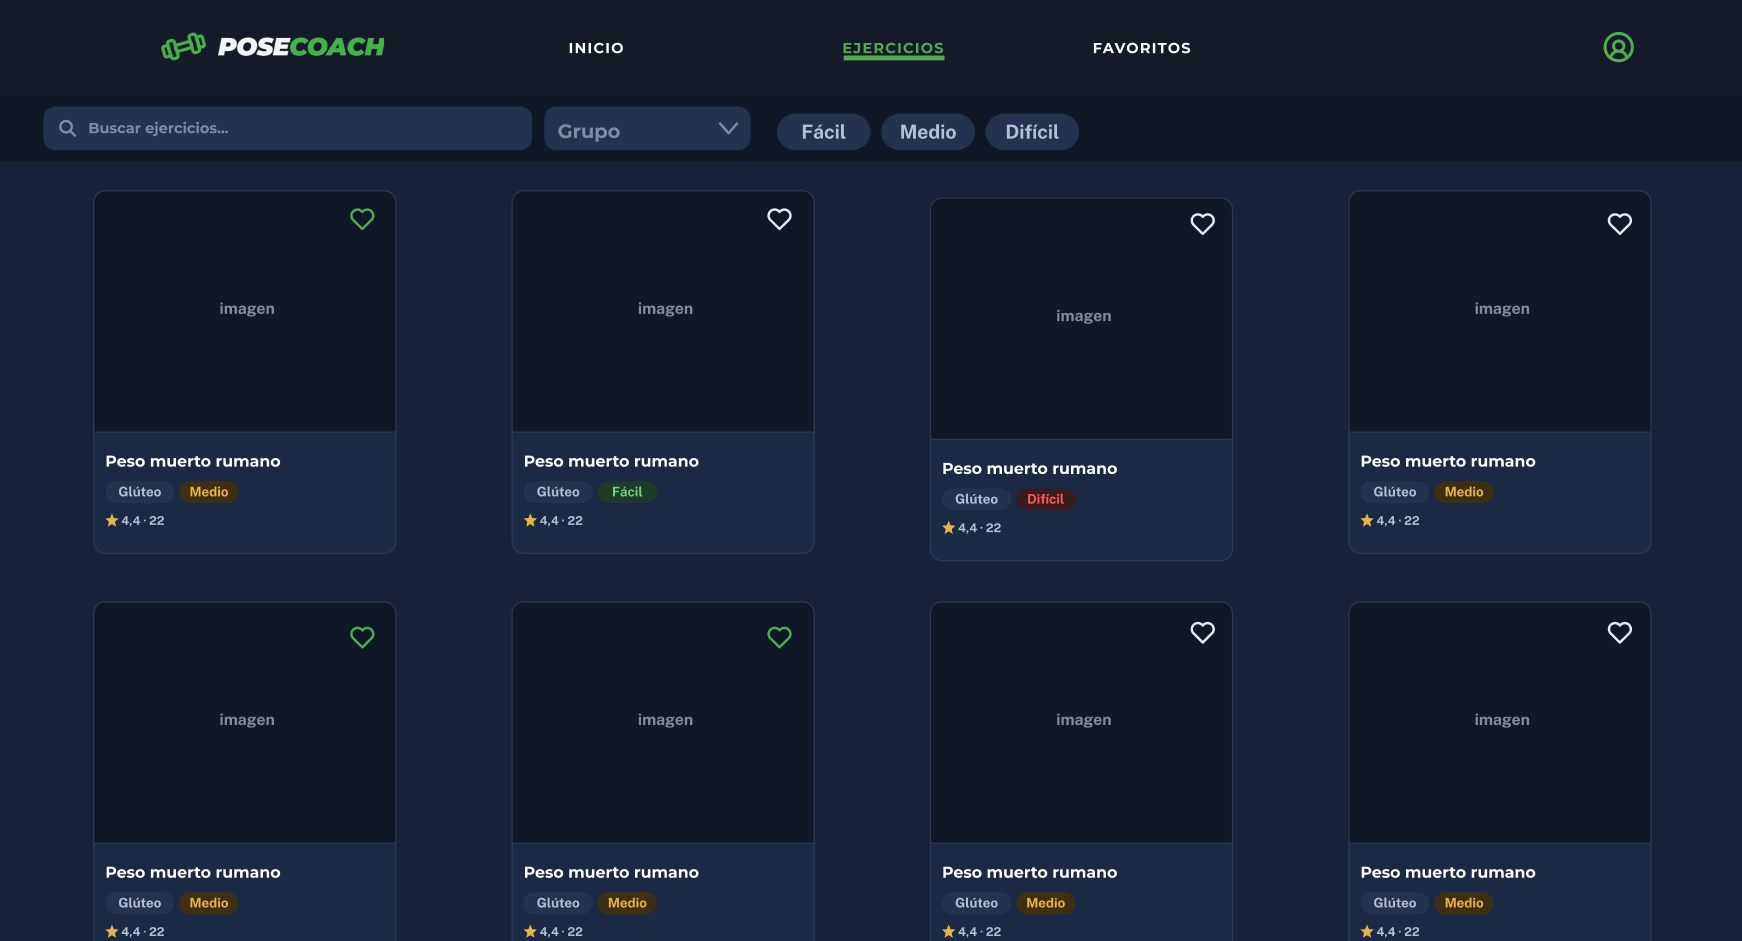
\includegraphics[width=\textwidth]{img/mockup-catalogo.png}
        \caption{Maqueta de la vista de catálogo, con la barra de filtros y la
        rejilla de tarjetas.}
        \label{fig:mockup-catalogo}
    \end{figure}

    El indicador de favorito presenta dos estados visuales: contorno sin
    relleno cuando el ejercicio no está marcado y silueta rellena en color de
    acento cuando sí lo está. Tanto este control como la valoración media se
    contemplaron desde el diseño inicial de la tarjeta, pese a corresponder a
    un incremento posterior, precisamente para no tener que rediseñarla al
    incorporarlos.

    La vista de catálogo contempla además tres situaciones distintas al margen
    del listado con resultados: la espera mientras se recuperan los datos, el
    fallo de comunicación con el servidor, que ofrece la posibilidad de
    reintentar la operación, y la ausencia de resultados. Este último caso
    distingue a su vez entre un catálogo vacío y una combinación de filtros
    sin coincidencias, ya que la acción que se espera del usuario es diferente
    en cada caso.

    La vista de detalle, recogida en la Figura~\ref{fig:mockup-detalle}, se
    estructura en una cabecera con el nombre y los distintivos del ejercicio y
    un conjunto de tres pestañas cuyo contenido corresponde a requisitos e
    incrementos distintos: \textit{Información} (RF-04), \textit{Analizar mi
    técnica} (RF-08) y \textit{Valoraciones} (RF-05 y RF-06). La pestaña de
    análisis solo se muestra en aquellos ejercicios que tienen un analizador
    postural asociado.

    \begin{figure}[htbp]
        \centering
        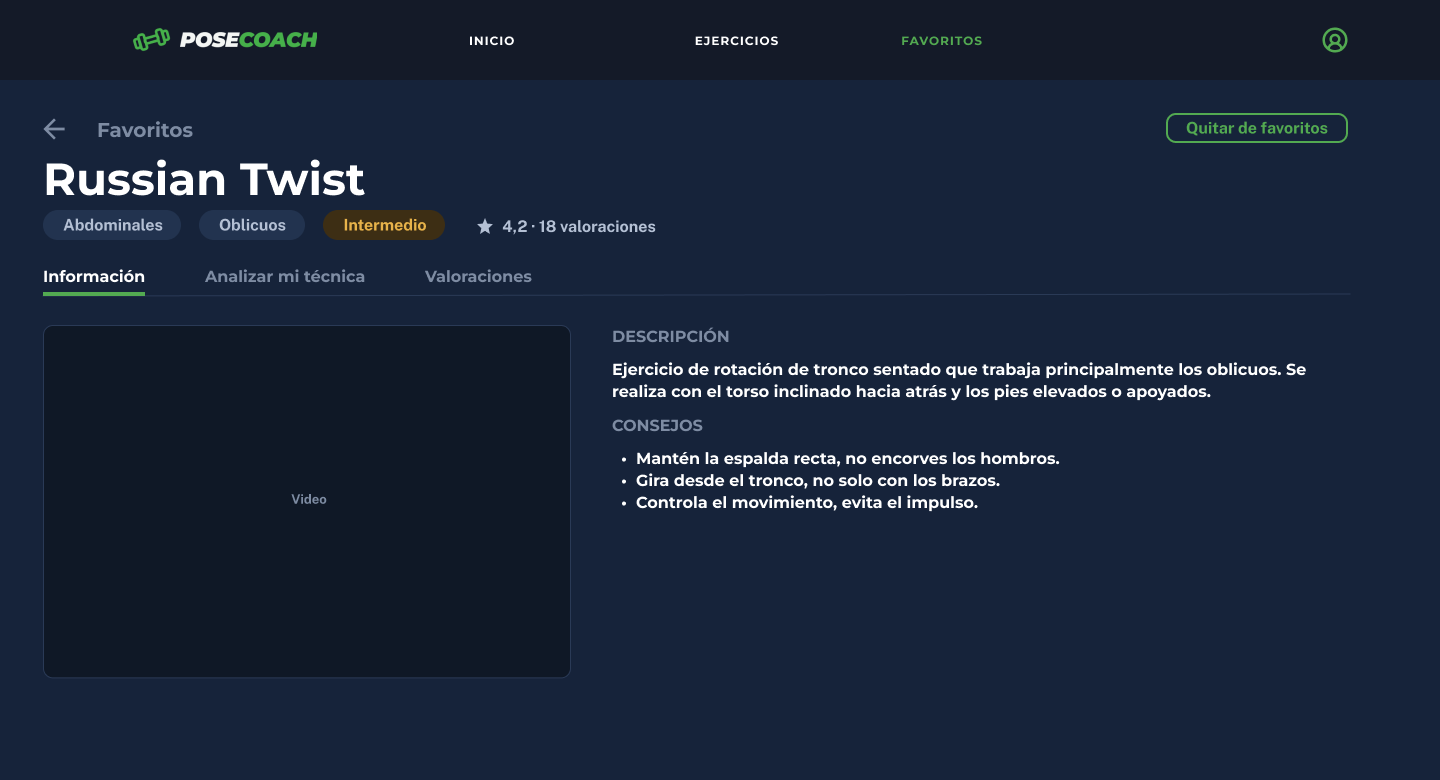
\includegraphics[width=\textwidth]{img/mockup-detalle.png}
        \caption{Maqueta de la vista de detalle de un ejercicio.}
        \label{fig:mockup-detalle}
    \end{figure}

    La navegación se organiza en torno a tres plantillas de página o
    \textit{layouts}, cada una con una cabecera distinta según el contexto: una
    plantilla pública para la página de presentación, con accesos a registro e
    inicio de sesión; una plantilla de autenticación para el registro y el
    inicio de sesión, que muestra únicamente el logotipo para minimizar
    distracciones durante el proceso; y una plantilla privada que incorpora el
    menú de navegación principal y el acceso al perfil del usuario. Cada vista
    se asocia a una de estas plantillas, lo que evita duplicar la estructura
    común y garantiza la coherencia visual entre pantallas del mismo tipo.

    El módulo de valoraciones y favoritos incorpora una vista adicional,
    recogida en la Tabla~\ref{tab:vistas-e3}, y añade contenido a la pestaña
    \textit{Valoraciones} de la vista de detalle, prevista desde el diseño
    inicial del catálogo.

    \begin{table}[htbp]
        \centering
        \begin{tabular}{lll}
            \toprule
            \textbf{Vista} & \textbf{Ruta} & \textbf{Acceso} \\
            \midrule
            Ejercicios favoritos & /favorites & Privada \\
            \bottomrule
        \end{tabular}
        \caption{Vista del módulo de valoraciones y favoritos.}
        \label{tab:vistas-e3}
    \end{table}

    La pestaña de valoraciones, cuya maqueta se recoge en la
    Figura~\ref{fig:mockup-valoraciones}, presenta tres bloques. A la
    izquierda, la valoración media acompañada de la distribución de
    puntuaciones, representada como cinco barras proporcionales al número de
    valoraciones de cada nivel. A la derecha, el formulario de valoración
    propia, que reúne en una sola acción la selección de estrellas y la
    redacción del comentario. Debajo, el listado de comentarios, paginado
    mediante un control que amplía la lista sin sustituirla.

    \begin{figure}[htbp]
        \centering
        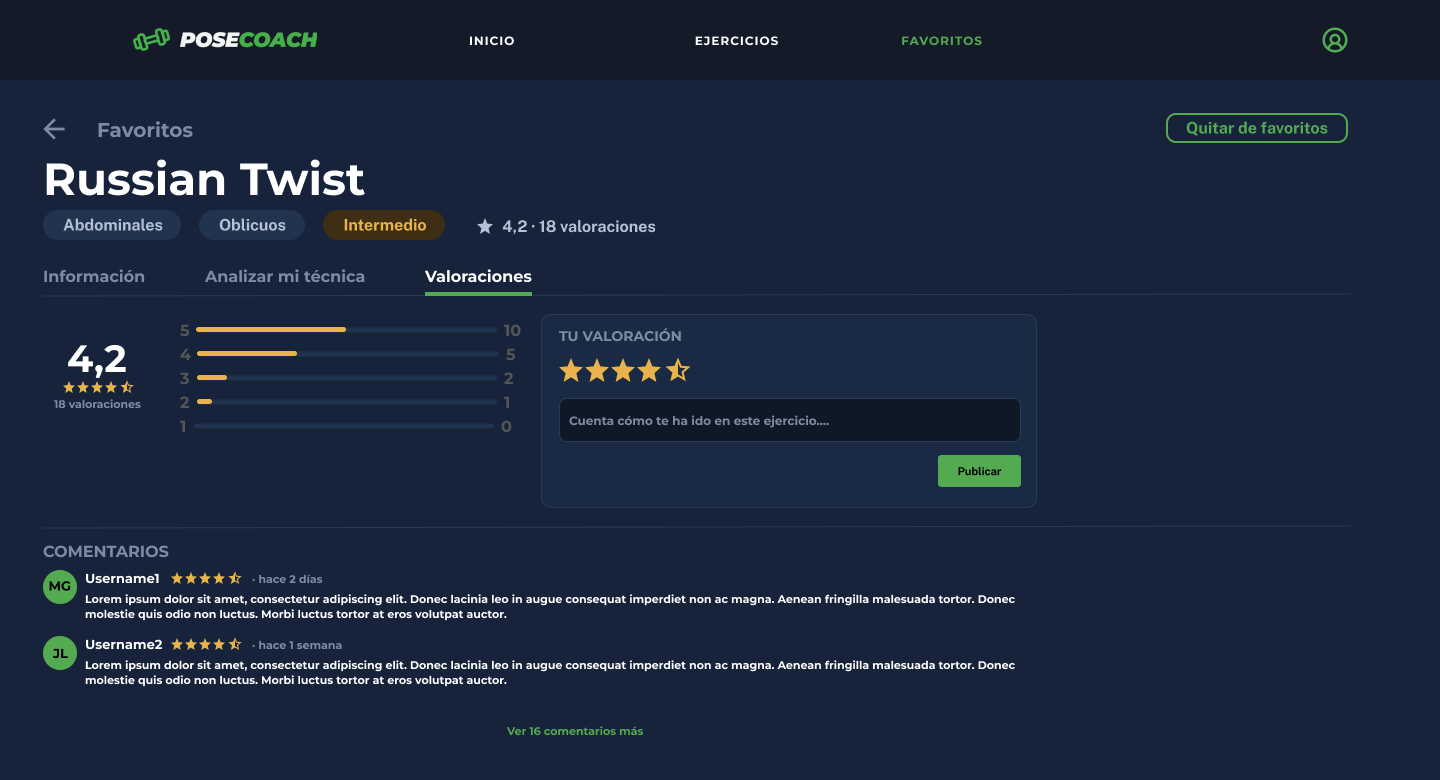
\includegraphics[width=\textwidth]{img/mockup-valoraciones.png}
        \caption{Maqueta de la pestaña de valoraciones de un ejercicio.}
        \label{fig:mockup-valoraciones}
    \end{figure}

    Cuando el usuario ya ha publicado su valoración, la pestaña adopta el
    estado recogido en la Figura~\ref{fig:mockup-valoraciones-publicada}: el
    formulario se muestra deshabilitado con los valores emitidos, y su
    comentario encabeza el listado, señalado como propio. Las acciones de
    edición y eliminación se sitúan en el formulario y no junto al comentario
    destacado, por dos motivos. El primero es de alcance: la eliminación afecta
    a la valoración completa, estrellas incluidas, y ubicarla junto al
    comentario sugeriría que solo retira el texto. El segundo es de cobertura:
    un usuario que haya puntuado sin escribir nada no genera comentario alguno,
    de modo que unas acciones ancladas al comentario lo dejarían sin ninguna
    forma de modificar o retirar su valoración.

    \begin{figure}[htbp]
        \centering
        \includegraphics[width=\textwidth]{img/mockup-valoraciones-publicada.png}
        \caption{Pestaña de valoraciones con una valoración ya publicada:
        formulario bloqueado con las acciones de edición y eliminación, y
        comentario propio destacado al inicio del listado.}
        \label{fig:mockup-valoraciones-publicada}
    \end{figure}

    Cada comentario se identifica mediante el nombre de su autor, un avatar
    generado a partir de sus iniciales y la antigüedad de la publicación
    expresada en términos relativos, más legible que una fecha absoluta en un
    listado de mensajes recientes. Los comentarios modificados con
    posterioridad a su publicación se señalan como tales.

    La vista de ejercicios favoritos, recogida en la
    Figura~\ref{fig:mockup-favoritos}, reutiliza íntegramente la rejilla de
    tarjetas y la barra de filtros del catálogo, conforme a lo anticipado en el
    diseño de la tarjeta como componente independiente. La barra de filtros
    solo se muestra a partir de dos ejercicios guardados, ya que filtrar un
    listado con un único elemento carece de utilidad; su presencia depende del
    total de favoritos y no del número de resultados visibles, de manera que un
    filtro que no arroje coincidencias siga pudiendo deshacerse.

    \begin{figure}[htbp]
        \centering
        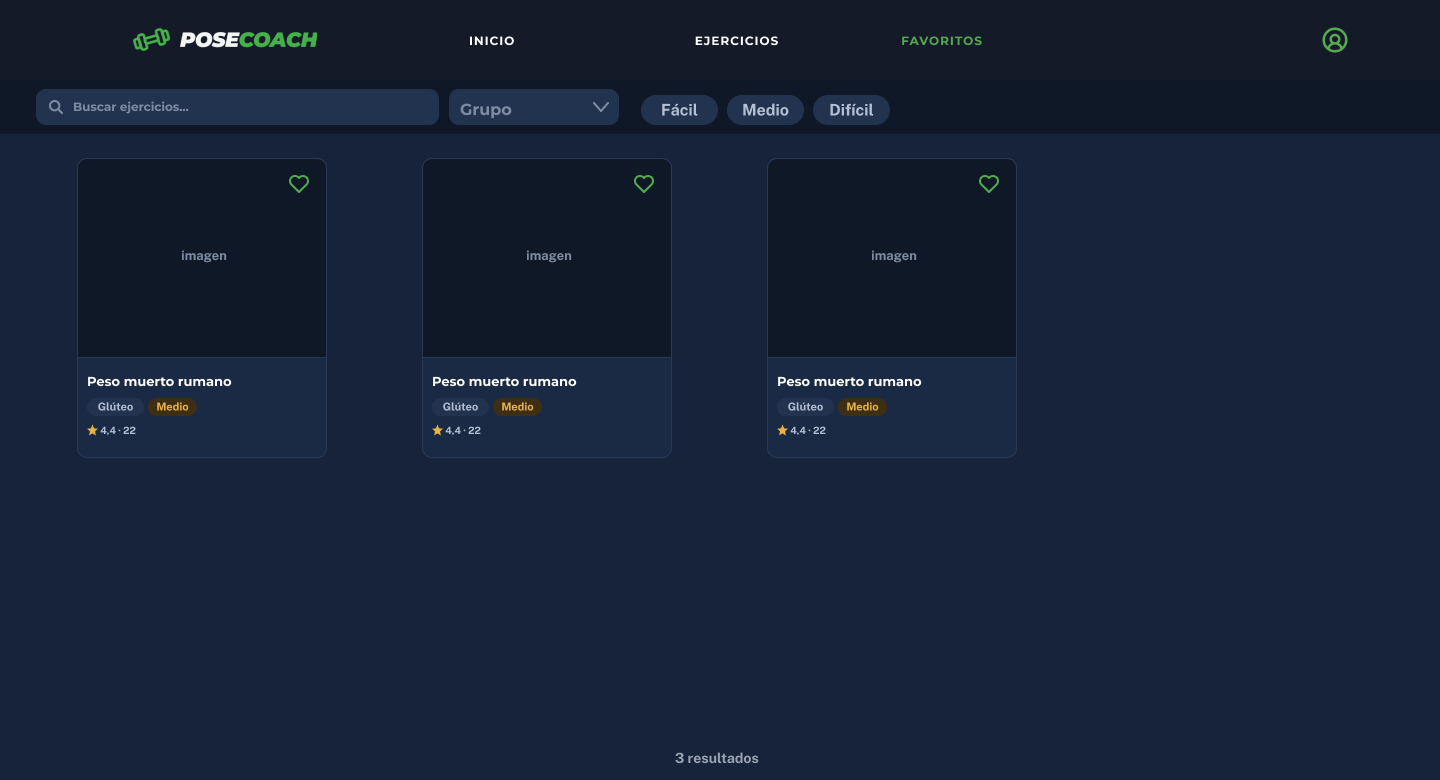
\includegraphics[width=\textwidth]{img/mockup-favoritos.png}
        \caption{Maqueta de la vista de ejercicios favoritos.}
        \label{fig:mockup-favoritos}
    \end{figure}

    Esta vista distingue dos situaciones de listado vacío que la interfaz no
    debe confundir, ya que la acción esperada del usuario es distinta en cada
    una. La ausencia de favoritos guardados, recogida en la
    Figura~\ref{fig:mockup-favoritos-vacio}, explica el funcionamiento del
    marcado y ofrece un acceso directo al catálogo; la ausencia de
    coincidencias con los filtros activos, en cambio, no invita a abandonar la
    vista, puesto que el contenido existe y lo que procede es modificar los
    criterios de búsqueda.

    \begin{figure}[htbp]
        \centering
        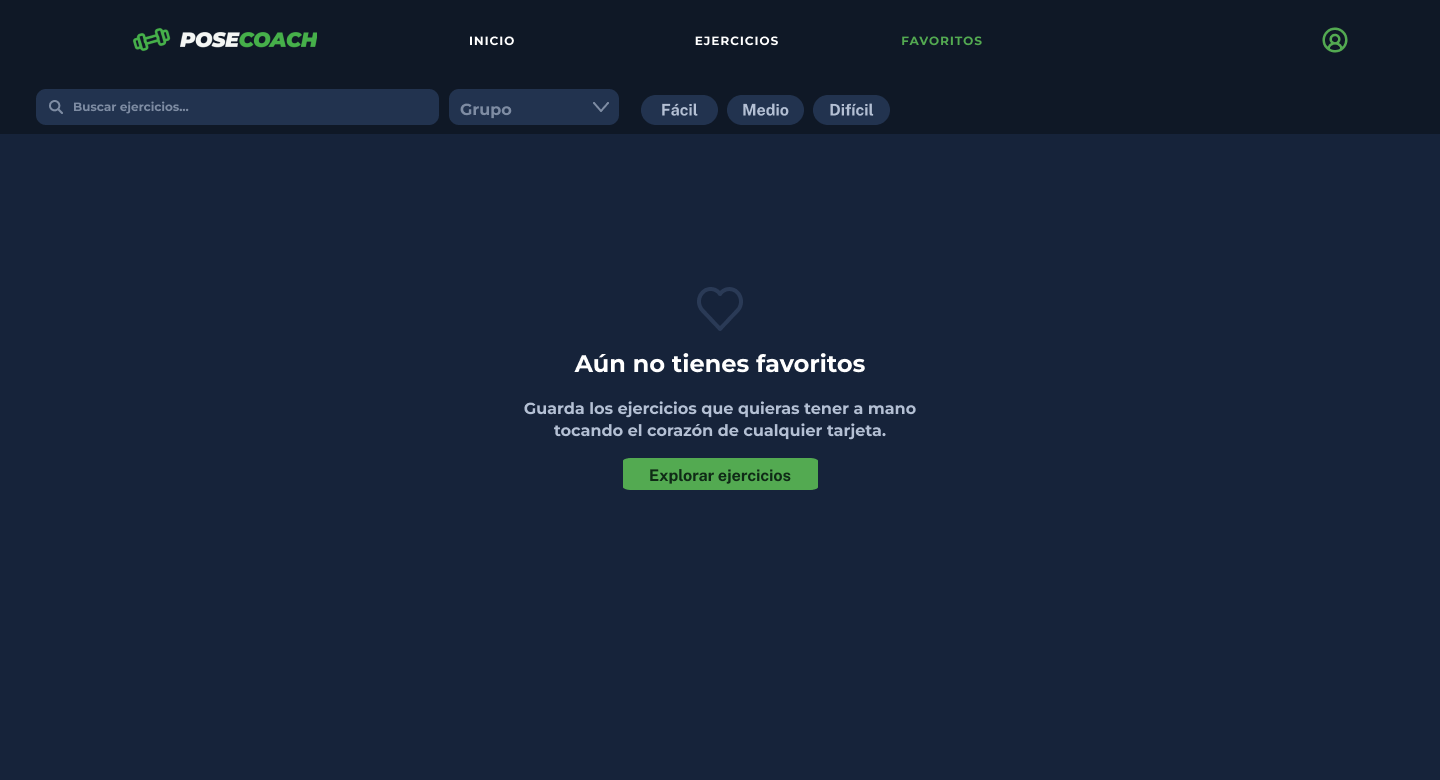
\includegraphics[width=\textwidth]{img/mockup-favoritos-vacio.png}
        \caption{Vista de ejercicios favoritos sin ningún ejercicio guardado.}
        \label{fig:mockup-favoritos-vacio}
    \end{figure}

    Por último, al retirar un ejercicio de favoritos desde esta vista su
    tarjeta desaparece de inmediato del listado. Se valoró la alternativa de
    mantenerla visible con el indicador desmarcado hasta la siguiente carga,
    lo que permitiría deshacer una pulsación accidental, pero se descartó por
    coherencia: una pantalla titulada «mis favoritos» no debería mostrar
    ejercicios que han dejado de serlo, y recuperar el marcado supone una única
    acción desde el catálogo.

    \section{Prototipado y sistema de diseño}

    Antes de implementar la interfaz se elaboró un prototipo de alta fidelidad
    de todas las pantallas con la herramienta Figma. El prototipado permite
    validar la disposición de los elementos, la coherencia visual y los flujos
    de navegación antes de escribir código, reduciendo el retrabajo durante el
    desarrollo.

    \subsection{Sistema de diseño}

    Se ha definido un sistema de diseño común que fija la paleta de colores, la
    tipografía y el estilo de los componentes reutilizables (botones, campos de
    formulario, tarjetas y mensajes de aviso), garantizando una apariencia
    homogénea en toda la aplicación. La interfaz adopta un tema oscuro; la
    Tabla~\ref{tab:paleta} recoge sus colores principales.

    \begin{table}[htbp]
        \centering
        \begin{tabular}{l l p{6.2cm}}
            \toprule
            \textbf{Uso} & \textbf{Color} & \textbf{Descripción} \\
            \midrule
            Fondo            & \#16233A & Fondo base de la aplicación \\
            Superficie       & \#1A2A44 & Tarjetas y formularios \\
            Cabecera         & \#141A28 & Barra de navegación \\
            Campos           & \#0F1826 & Fondo de los campos de formulario \\
            Texto            & \#E6EBF2 & Texto principal \\
            Texto secundario & \#8B98AD & Textos de apoyo y ayudas \\
            Acento           & \#3FB950 & Elementos interactivos y estados positivos \\
            Texto sobre acento & \#0D1F12 & Texto sobre superficies de color de acento \\
            Aviso            & \#E3B341 & Advertencias \\
            Error            & \#F85149 & Mensajes y estados de error \\
            \bottomrule
        \end{tabular}
        \caption{Paleta de colores del sistema de diseño.}
        \label{tab:paleta}
    \end{table}

    La jerarquía visual se apoya en la luminosidad de las superficies: la barra
    de navegación y los campos de formulario emplean tonos más oscuros que el
    fondo, mientras que las tarjetas utilizan un tono más claro, lo que
    transmite la sensación de que estas se sitúan por encima del plano de la
    página.

    Como decisión de accesibilidad, el verde de acento se reserva
    exclusivamente para elementos interactivos y estados positivos, mientras
    que el texto principal emplea un tono claro (\#E6EBF2) que garantiza una
    relación de contraste suficiente sobre el fondo oscuro. Utilizar el color
    de acento para el texto corrido habría comprometido la legibilidad.

    La materialización del sistema de diseño en el cliente distingue dos
    ámbitos. Los estilos propios de cada componente permanecen encapsulados en
    él, de modo que no puedan afectar al resto de la aplicación. Los elementos
    que se repiten en pantallas distintas, en cambio, se declaran una sola vez
    como clases globales: es el caso de los distintivos de grupo muscular y
    dificultad, del botón de acción principal y de una utilidad de ocultación
    visual que mantiene un contenido accesible para los lectores de pantalla
    sin representarlo gráficamente. Esta última se emplea en la vista de
    favoritos, cuyo diseño prescinde de un título visible pero que, como toda
    página, requiere un encabezado que permita identificarla mediante
    tecnologías de asistencia.

    \subsection{Maquetas de las pantallas}

    A continuación se muestran las maquetas de las pantallas diseñadas en
    Figma, que han servido de referencia directa durante la implementación de
    la interfaz.

C   onviene precisar que el prototipo abarca el alcance funcional completo
    previsto para la aplicación, y no únicamente el del incremento descrito en
    este capítulo. Algunas de las pantallas incluyen, por tanto, elementos cuya
    implementación corresponde a incrementos posteriores, como el resumen de
    análisis posturales recientes de la página de inicio. Esta anticipación es
    deliberada: diseñar la interfaz de forma global desde el inicio permite
    establecer un sistema de diseño coherente y dimensionar correctamente cada
    pantalla, evitando rediseños parciales a medida que el proyecto avanza.

    \begin{figure}[htbp]
        \centering
        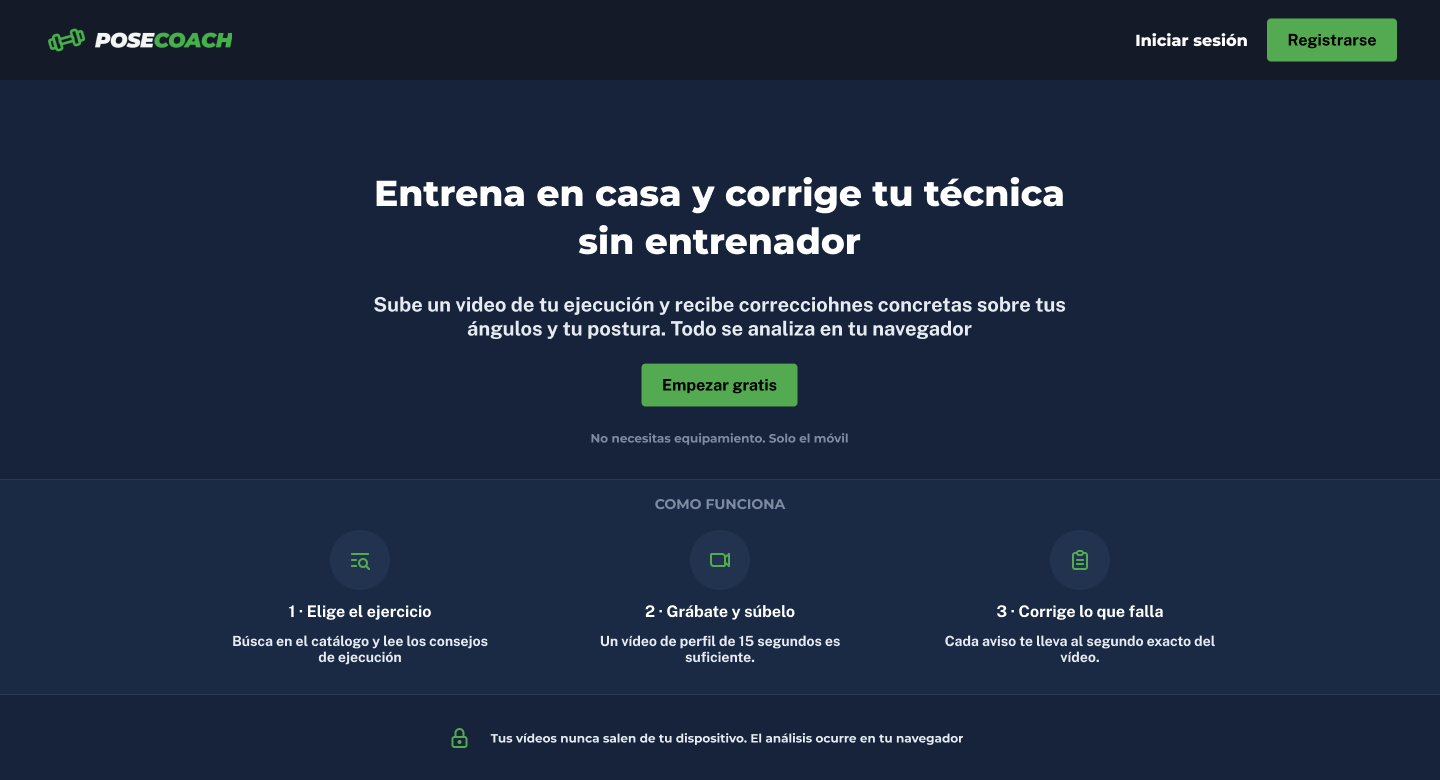
\includegraphics[width=\textwidth]{img/mockup-home.png}
        \caption{Maqueta de la página de presentación (usuario no autenticado).}
        \label{fig:mockup-home}
    \end{figure}

    \begin{figure}[htbp]
        \centering
        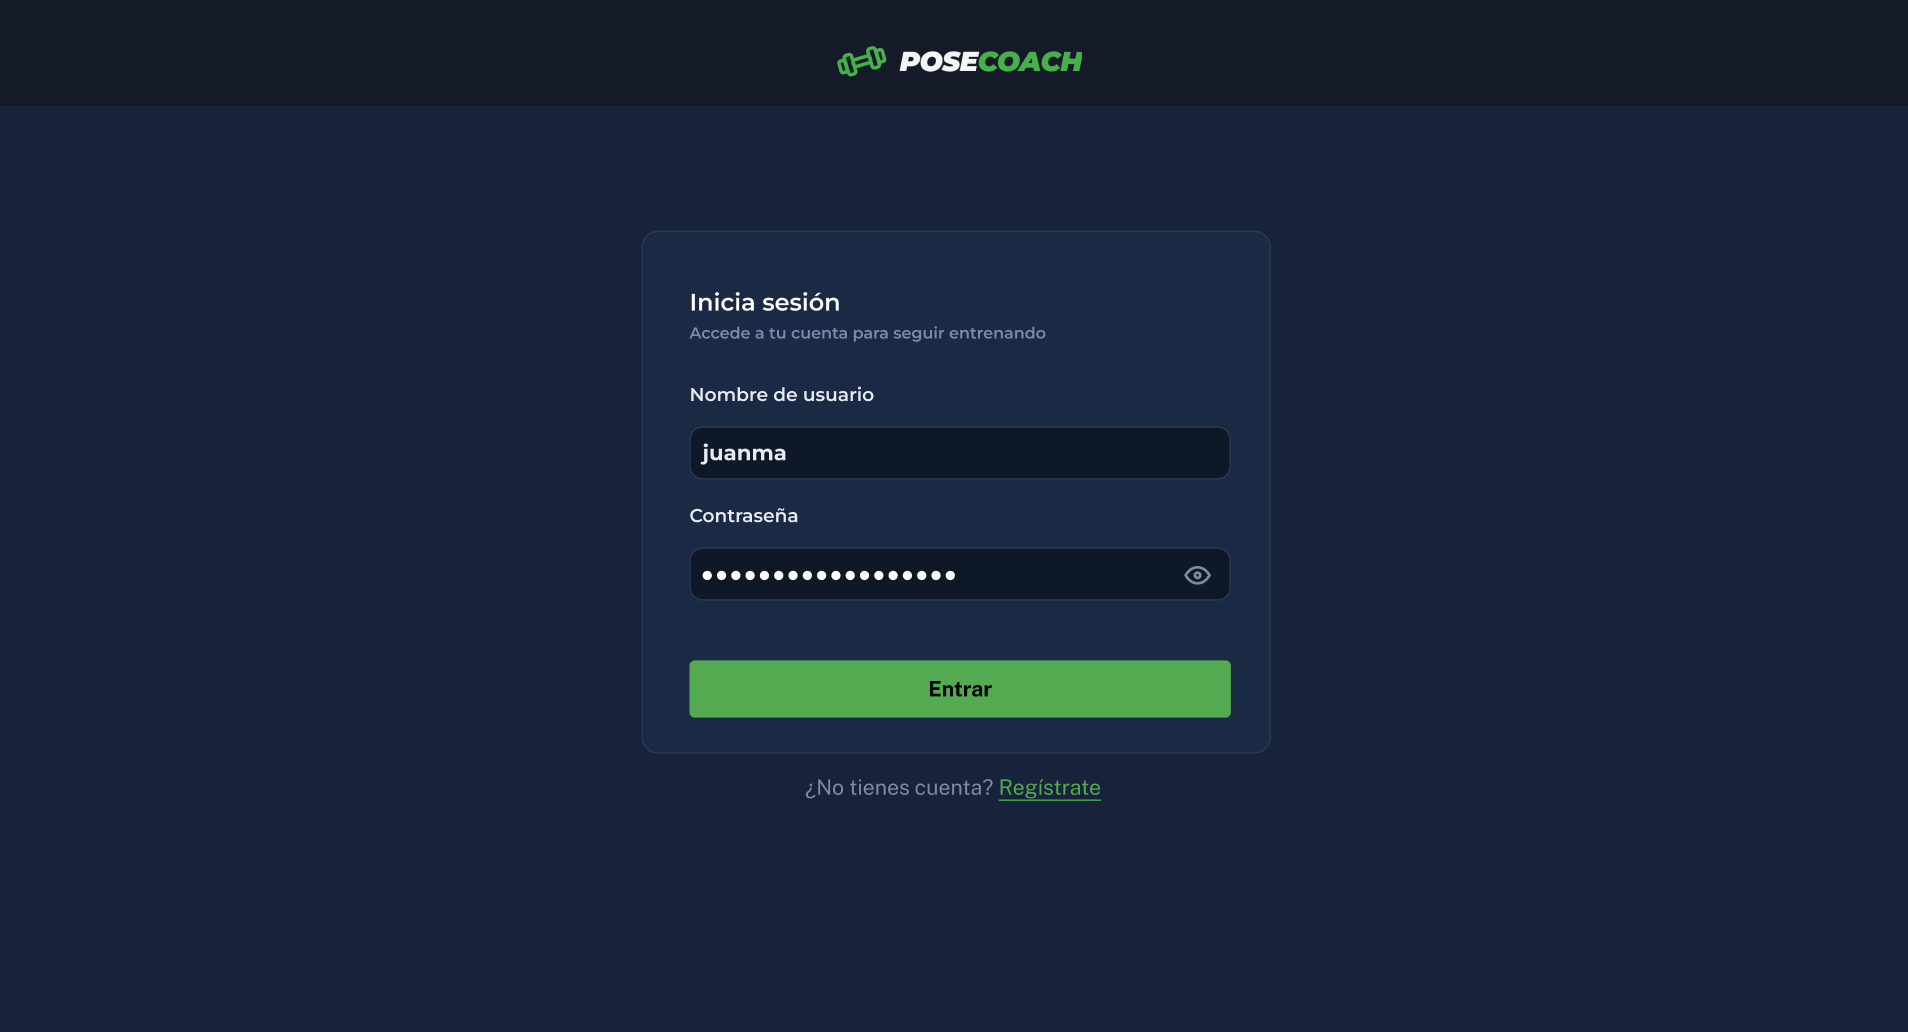
\includegraphics[width=0.7\textwidth]{img/mockup-login.png}
        \caption{Maqueta de la pantalla de inicio de sesión.}
        \label{fig:mockup-login}
    \end{figure}

    \begin{figure}[htbp]
        \centering
        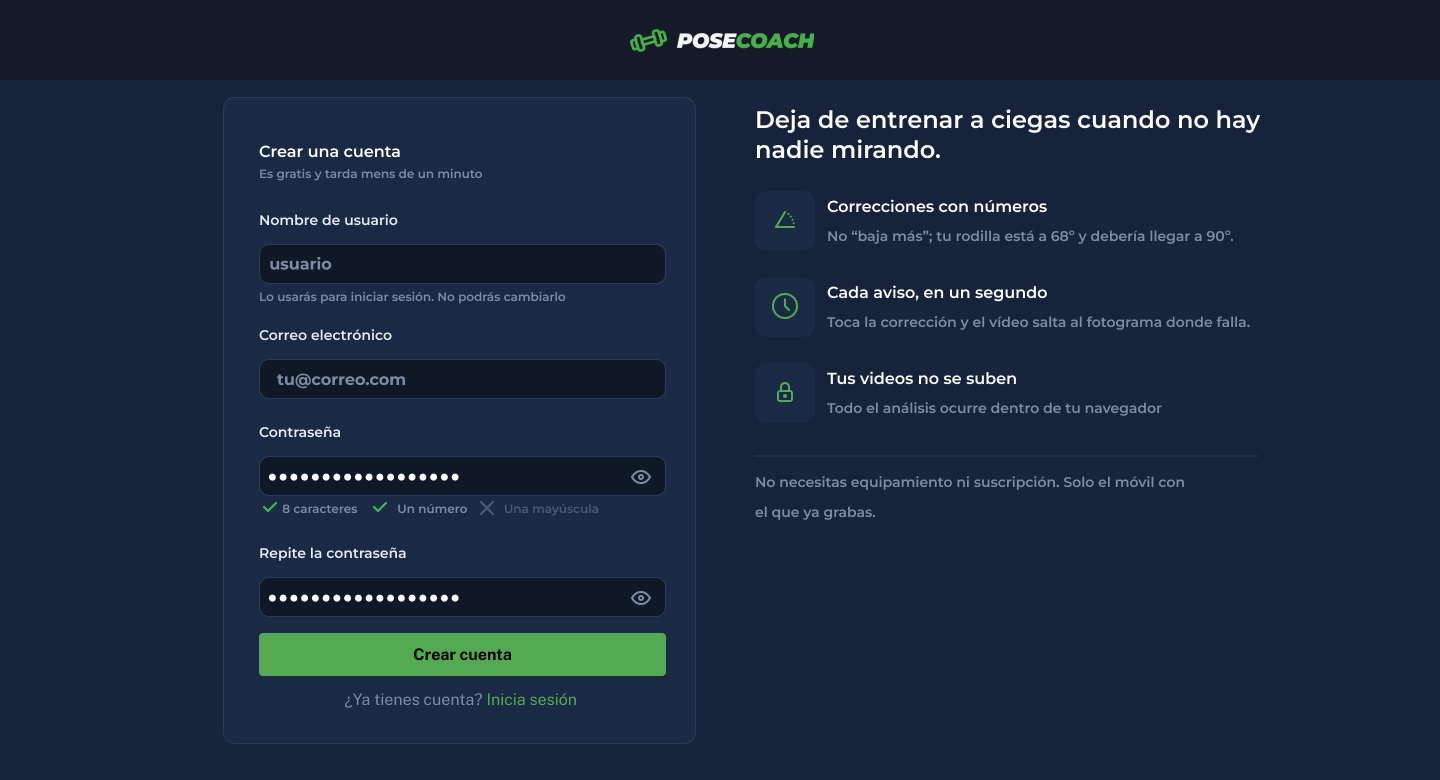
\includegraphics[width=\textwidth]{img/mockup-registro.png}
        \caption{Maqueta de la pantalla de registro, con los indicadores de
        cumplimiento de la política de contraseña.}
        \label{fig:mockup-registro}
    \end{figure}

    \begin{figure}[htbp]
        \centering
        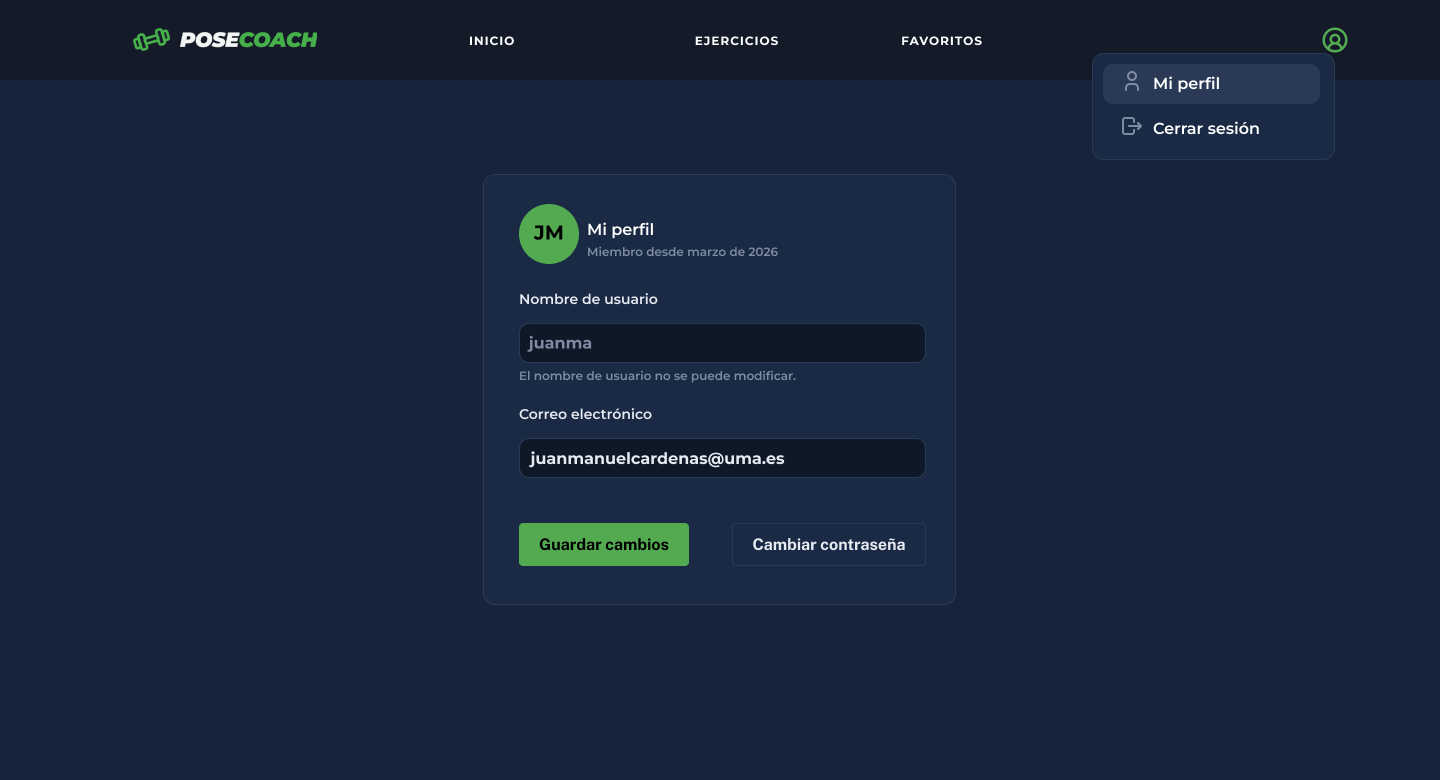
\includegraphics[width=\textwidth]{img/mockup-perfil.png}
        \caption{Maqueta del perfil de usuario, con el menú de cuenta
        desplegado.}
        \label{fig:mockup-perfil}
    \end{figure}


    \section{Diseño del módulo de corrección postural}


% ─────────────────────── Capítulo 6 ──────────────────────────────────


    \chapter{Implementación}
    \label{cap:implementacion}

    \section{Puesta en marcha del entorno}

    El primer incremento no produjo funcionalidad visible, sino la
    infraestructura sobre la que se construyen los demás. Se creó un
    repositorio único (\textit{monorepo}) que agrupa el cliente, el servidor y
    la documentación, decisión que mantiene sincronizados en un mismo cambio
    los ajustes que afectan a ambos extremos, como una modificación del
    contrato de la API. Sobre él se generaron los esqueletos de ambos
    proyectos y se levantó la base de datos en un contenedor Docker con volumen
    persistente, de modo que el entorno completo pueda reproducirse en
    cualquier máquina sin instalaciones manuales.

    \subsection{Validación técnica previa del análisis postural}

    Antes de comprometer la arquitectura del sistema se realizó una prueba de
    concepto (\textit{spike}) del componente de mayor riesgo técnico del
    proyecto: la estimación de pose en el navegador. La razón es que el
    requisito no funcional RNF-02 condiciona toda la arquitectura al exigir que
    los vídeos no abandonen el dispositivo del usuario; si el procesamiento en
    el navegador hubiera resultado inviable, habría sido necesario replantear
    el sistema por completo, y descubrirlo en las últimas semanas habría
    comprometido el proyecto.

    La prueba consistió en una página independiente que carga el modelo
    PoseLandmarker de MediaPipe, procesa un vídeo local, detecta los puntos
    clave del cuerpo y calcula a partir de ellos el ángulo de flexión de la
    rodilla. Su resultado confirmó tanto la viabilidad del enfoque como la
    disponibilidad de las magnitudes necesarias para evaluar la técnica de
    ejecución, permitiendo continuar con el resto de incrementos sin
    incertidumbre sobre el objetivo principal del trabajo.

    \begin{figure}[htbp]
        \centering
        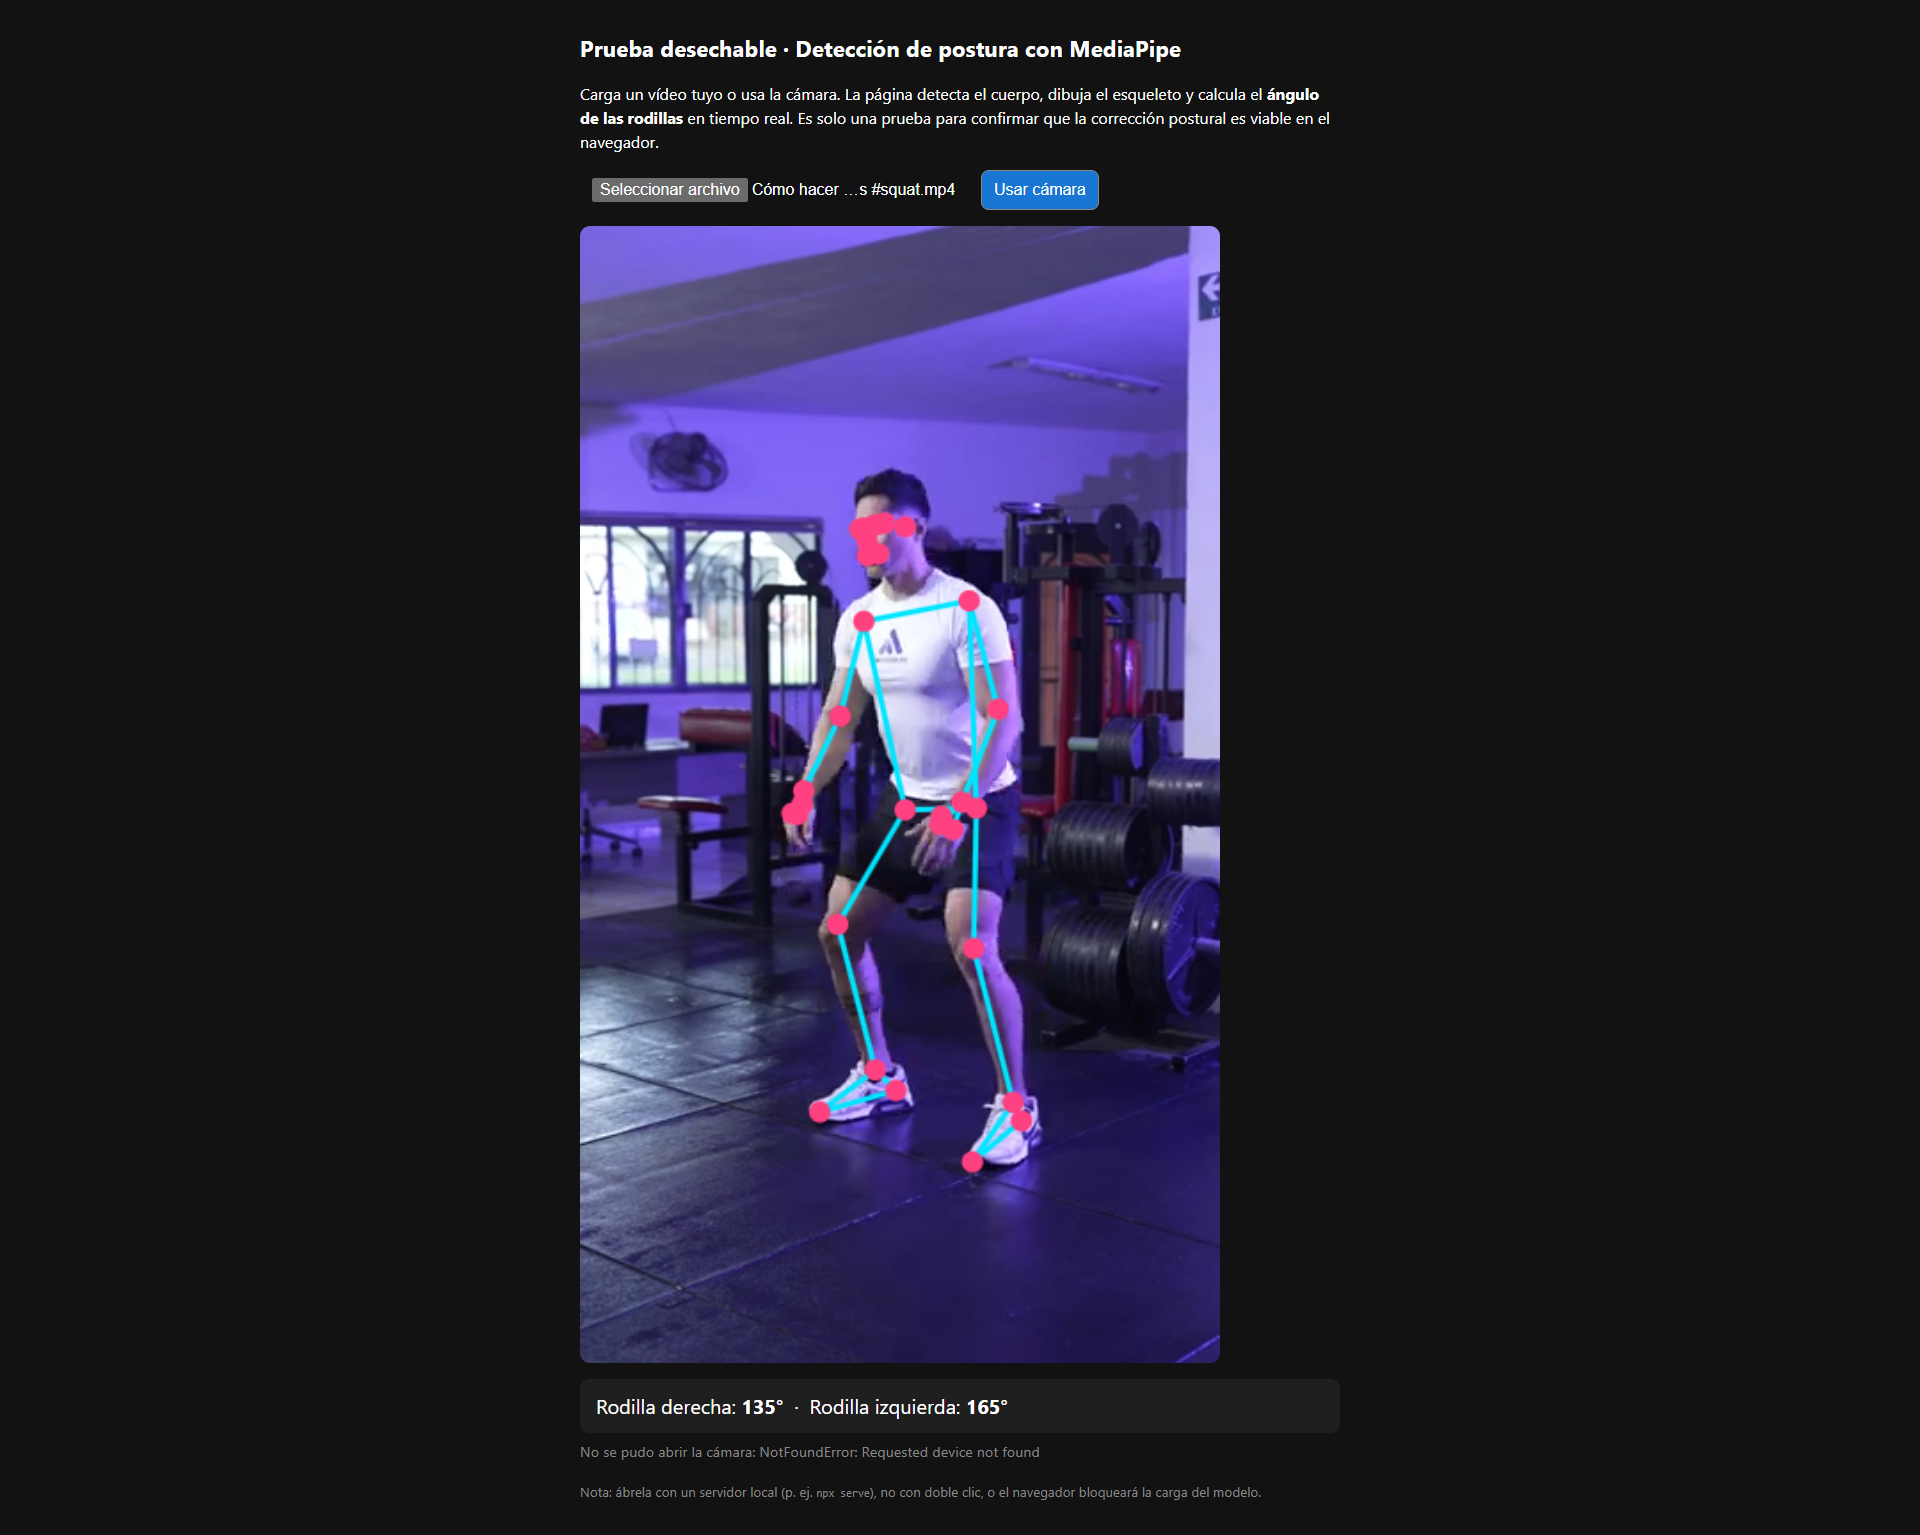
\includegraphics[width=0.85\textwidth]{img/spike-mediapipe.png}
        \caption{Prueba de concepto de estimación de pose en el navegador:
        detección de los puntos clave del cuerpo y cálculo del ángulo de la
        rodilla sobre un vídeo local.}
        \label{fig:spike-mediapipe}
    \end{figure}


    \section{Gestión de usuarios y autenticación}
El primer módulo implementado en el backend es el de gestión de usuarios,
    que constituye la base sobre la que se apoya el resto de funcionalidades
    del sistema. En esta primera fase se construyó el modelo de dominio y la
    capa de persistencia; sobre ellos se implementó después el registro de
    usuarios.

    \subsection{Modelo de dominio y persistencia}

    La entidad \texttt{User}, cuyos atributos se recogieron en la
    Tabla~\ref{tab:entidad-user}, se ha implementado como una entidad JPA
    (\textit{Java Persistence API}) anotada con \texttt{@Entity} y mapeada a la
    tabla \texttt{users}. Se ha optado por el nombre en plural porque
    \texttt{user} es una palabra reservada en MySQL, lo que evita conflictos en
    las consultas SQL generadas.

    El atributo \texttt{role} se persiste como cadena de texto mediante la
    anotación \texttt{@Enumerated(EnumType.STRING)}, de modo que en la base de
    datos se almacenan los valores \texttt{USER} y \texttt{ADMIN} de forma
    legible en lugar de un índice numérico. Los campos \texttt{username} y
    \texttt{email} se declaran con la restricción \texttt{unique}, garantizando
    su unicidad a nivel de base de datos. La fecha de alta (\texttt{createdAt})
    se asigna automáticamente antes de la primera inserción mediante un método
    anotado con \texttt{@PrePersist}. Para reducir el código repetitivo
    (\textit{getters}, \textit{setters} y constructores) se emplea la
    biblioteca Lombok.

    El acceso a los datos se delega en la interfaz \texttt{UserRepository}, que
    extiende \texttt{JpaRepository} de Spring Data JPA. Esta herencia
    proporciona automáticamente las operaciones CRUD básicas, a las que se
    añaden los métodos de consulta derivados recogidos en la
    Tabla~\ref{tab:user-repository}, cuya implementación genera Spring a partir
    del nombre del método sin necesidad de escribir SQL.

    \begin{table}[htbp]
        \centering
        \begin{tabular}{ll}
            \toprule
            \textbf{Método} & \textbf{Función} \\
            \midrule
            findByUsername   & Recupera un usuario por su nombre de usuario \\
            findByEmail      & Recupera un usuario por su correo electrónico \\
            existsByUsername & Comprueba si un nombre de usuario ya existe \\
            existsByEmail    & Comprueba si un correo ya está registrado \\
            \bottomrule
        \end{tabular}
        \caption{Métodos de consulta de \texttt{UserRepository}.}
        \label{tab:user-repository}
    \end{table}

    La generación del esquema se ha delegado en Hibernate mediante la propiedad
    \texttt{spring.jpa.hibernate.ddl-auto=update}, que crea y actualiza las
    tablas a partir de las entidades al arrancar la aplicación. Tras el primer
    arranque se verificó en la base de datos MySQL, ejecutada en un contenedor
    Docker, la creación correcta de la tabla \texttt{users} con las columnas y
    restricciones esperadas (Figura~\ref{fig:tabla-user-creacion}).

    \begin{figure}[htbp]
        \centering
        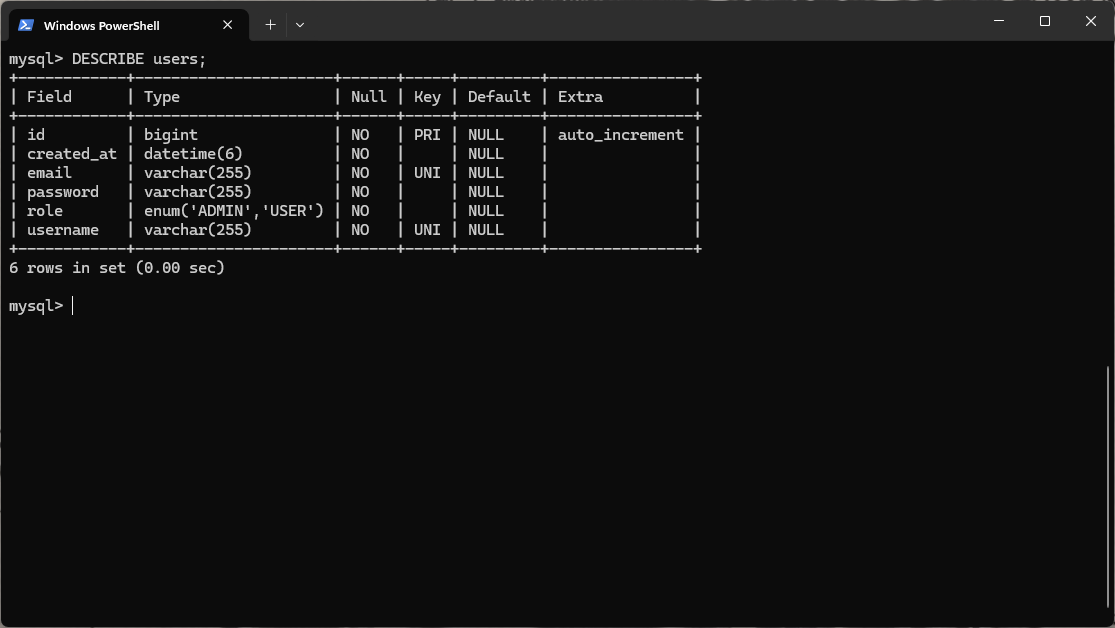
\includegraphics[width=0.85\textwidth]{img/tabla-user-creacion.png}
        \caption{Estructura de la tabla \texttt{users} generada por Hibernate,
        verificada con \texttt{DESCRIBE users} en MySQL.}
        \label{fig:tabla-user-creacion}
    \end{figure}

    \subsection{Registro de usuarios y cifrado de contraseñas}

    El registro se implementa siguiendo una separación en capas. El controlador
    \texttt{AuthController} expone el endpoint \texttt{POST /api/auth/register} y
    recibe los datos en un objeto de transferencia (\textit{DTO})
    \texttt{RegisterRequest}, en lugar de la entidad \texttt{User} directamente.
    Así, el cliente solo puede enviar el nombre de usuario, el correo y la
    contraseña, y nunca campos sensibles como el identificador o el rol. Los
    datos se validan de forma declarativa mediante anotaciones de Jakarta Bean Validation (\texttt{@NotBlank}, \texttt{@Email},
    \texttt{@Size} y \texttt{@Pattern}), de modo que un correo con formato
    incorrecto, una contraseña demasiado corta o una contraseña que no cumple
    la política de complejidad se rechazan antes de procesar la petición. Dicha
    política exige un mínimo de ocho caracteres e incluir al menos una letra
    minúscula, una mayúscula y un dígito, y se aplica por igual en el registro
    y en el cambio de contraseña, de forma que ambas operaciones garantizan el
    mismo nivel mínimo de seguridad.
    
    La lógica de negocio reside en el servicio \texttt{AuthService}, que
    comprueba mediante el repositorio si el nombre de usuario o el correo ya
    existen y, en caso afirmativo, interrumpe el registro. Si los datos son
    válidos y únicos, cifra la contraseña y persiste el nuevo usuario con el rol
    \texttt{USER} por defecto.

    El cifrado de la contraseña es un aspecto central de la seguridad del
    sistema. Almacenarla en texto plano supondría un riesgo grave: si la base de
    datos se viera comprometida, todas las credenciales quedarían expuestas. Por
    ello se emplea BCrypt, una función de \textit{hash} diseñada específicamente
    para contraseñas. BCrypt es unidireccional, esto quiere decir que no permite recuperar la
    contraseña original a partir del \textit{hash}, incorpora una \textit{sal}
    (\textit{salt}) aleatoria que evita que dos contraseñas iguales produzcan el
    mismo resultado, y su coste de cálculo es ajustable, lo que la hace
    resistente a ataques de fuerza bruta. En la aplicación, el cifrado se realiza
    mediante un \texttt{BCryptPasswordEncoder} declarado como \textit{bean} de
    Spring. La Figura~\ref{fig:bcrypt-hash} muestra el resultado en la base de
    datos: la contraseña se almacena como un \textit{hash} con el prefijo
    \texttt{\$2a\$}, característico de BCrypt, y no en texto legible.

    \begin{figure}[htbp]
        \centering
        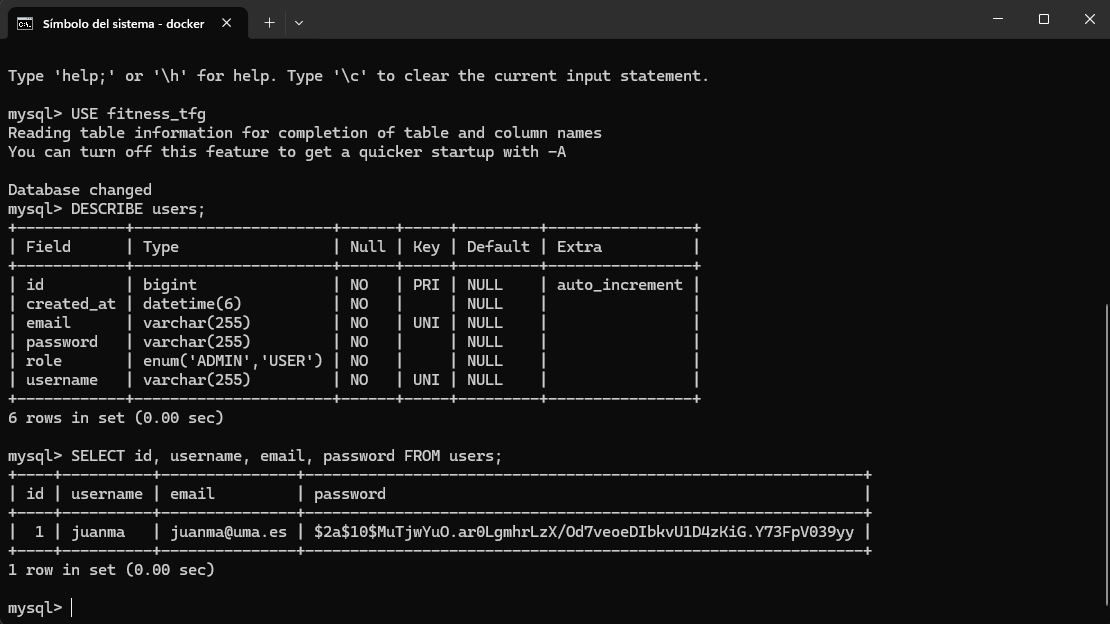
\includegraphics[width=0.95\textwidth]{img/bcrypt-hash.png}
        \caption{Contraseña almacenada cifrada con BCrypt en la tabla
        \texttt{users}, verificada mediante una consulta \texttt{SELECT}.}
        \label{fig:bcrypt-hash}
    \end{figure}

    Por último, las respuestas del endpoint se normalizan mediante un manejador
    global de excepciones (\texttt{@RestControllerAdvice}), que traduce los
    errores de validación a \texttt{400 Bad Request} y los conflictos de
    duplicado a \texttt{409 Conflict}, devolviendo en ambos casos un mensaje
    descriptivo en formato JSON.

    \subsection{Configuración de Spring Security}

    Al incorporar Spring Security, el marco protege por defecto todos los
    endpoints, lo que en un primer momento impedía el acceso al registro. Fue
    necesario definir una configuración explícita (\texttt{SecurityConfig}) que
    declara públicas las rutas bajo \texttt{/api/auth/**} y mantiene protegidas
    el resto. Además, al tratarse de una API REST sin estado, se deshabilitó la
    protección CSRF, cuyo propósito es evitar peticiones fraudulentas en
    formularios con sesión, no aplica en este modelo y, de mantenerse activa,
    bloquea las peticiones POST. La ausencia inicial de esta configuración se
    manifestó como respuestas \texttt{403 Forbidden}, lo que permitió identificar
    y corregir el problema durante la puesta en marcha.

    \subsection{Inicio de sesión y control de acceso}

    El inicio de sesión se implementa en el endpoint
    \texttt{POST /api/auth/login}. El servicio localiza al usuario por su nombre
    y compara la contraseña recibida con el \textit{hash} almacenado mediante el
    método \texttt{matches} del codificador BCrypt, que vuelve a cifrar la
    contraseña y contrasta el resultado sin necesidad de descifrar la original.
    Si las credenciales son válidas, se genera un token JWT firmado que incluye
    el nombre de usuario y el rol, y que se devuelve al cliente
    (Figura~\ref{fig:login-ok}); en caso contrario se responde con
    \texttt{401 Unauthorized}.

    \begin{figure}[htbp]
        \centering
        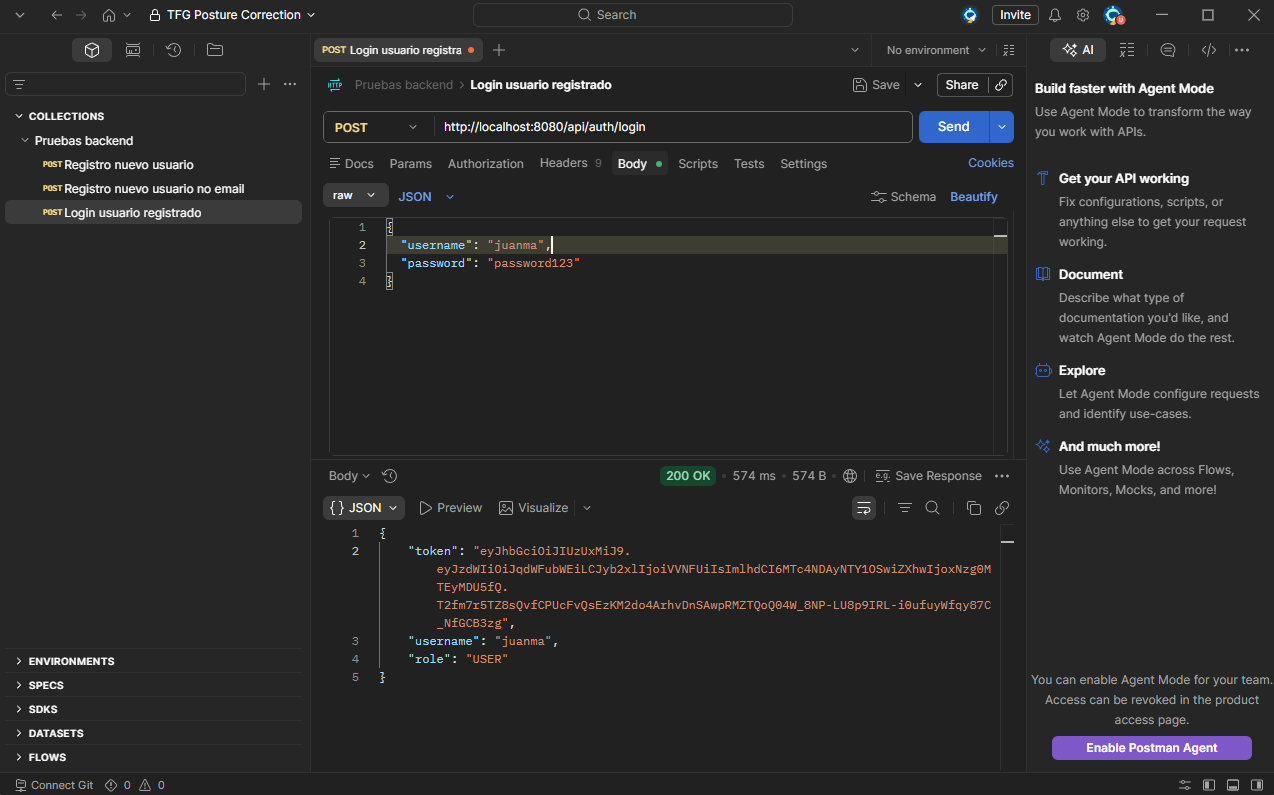
\includegraphics[width=0.9\textwidth]{img/login-ok.png}
        \caption{Inicio de sesión correcto: respuesta \texttt{200 OK} con el
        token JWT emitido.}
        \label{fig:login-ok}
    \end{figure}

    La generación y verificación de los tokens se centraliza en el componente
    \texttt{JwtService}, apoyado en la biblioteca jjwt. El control de acceso a
    las rutas protegidas se realiza mediante un filtro
    (\texttt{JwtAuthenticationFilter}) que se ejecuta en cada petición: extrae el
    token de la cabecera \texttt{Authorization}, verifica su firma y su vigencia,
    y, si es válido, establece la identidad del usuario en el contexto de
    seguridad de Spring. La configuración se establece en modo \textit{stateless}
    y declara públicas únicamente las rutas de autenticación, de modo que
    cualquier otra ruta exige un token válido.

    Este comportamiento se comprobó accediendo a una ruta protegida
    (\texttt{GET /api/users/me}) en dos situaciones. Sin un token válido, el
    servidor deniega el acceso (Figura~\ref{fig:ruta-sin-token}); presentando el
    token obtenido en el inicio de sesión, el servidor autoriza la petición y
    devuelve los datos del usuario (Figura~\ref{fig:ruta-con-token}).

    \begin{figure}[htbp]
        \centering
        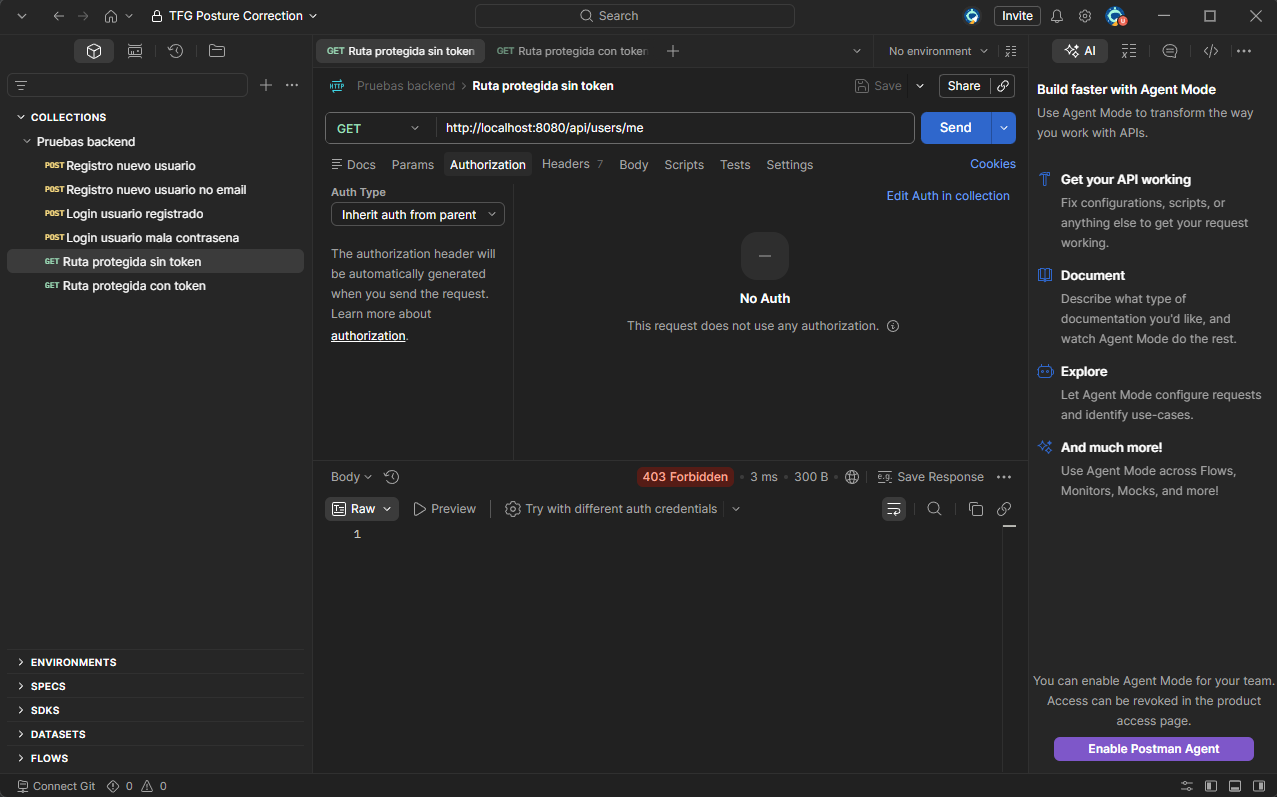
\includegraphics[width=0.9\textwidth]{img/ruta-sin-token.png}
        \caption{Acceso a una ruta protegida sin token: el servidor deniega la
        petición.}
        \label{fig:ruta-sin-token}
    \end{figure}

    \begin{figure}[htbp]
        \centering
        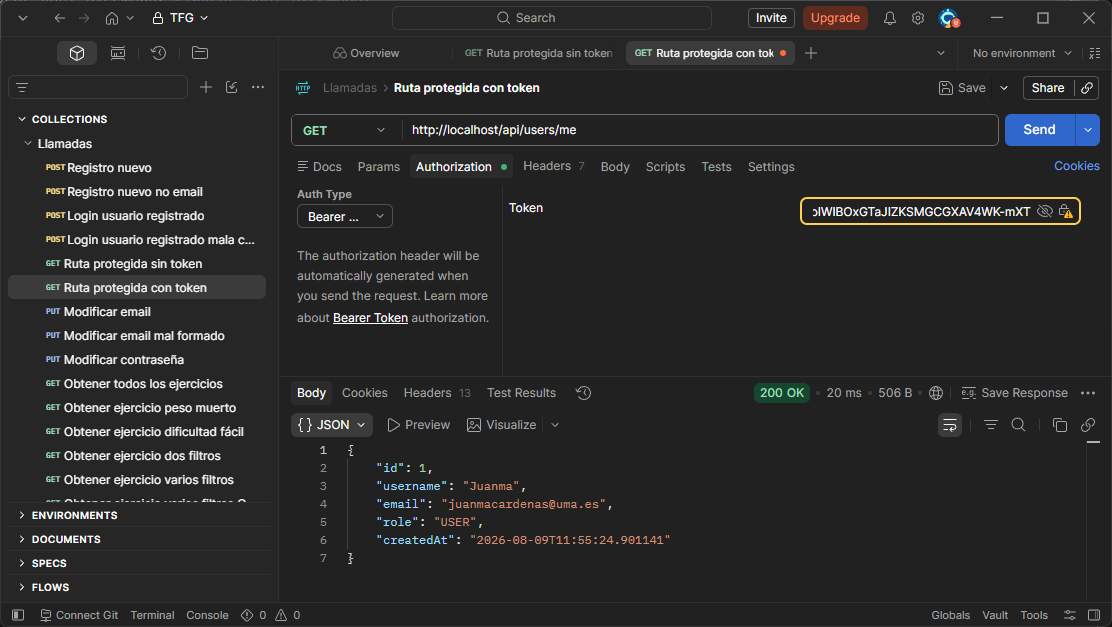
\includegraphics[width=0.9\textwidth]{img/ruta-con-token.png}
        \caption{Acceso a la misma ruta protegida presentando un token JWT
        válido: el servidor autoriza y devuelve los datos del usuario.}
        \label{fig:ruta-con-token}
    \end{figure}

    La integración con el cliente web hizo necesarios dos ajustes adicionales en
    la configuración de seguridad, ambos detectados durante la puesta en marcha
    del frontend.

    El primero es la configuración de CORS (\textit{Cross-Origin Resource
    Sharing}). Durante el desarrollo, el frontend se sirve en el puerto 4200 y
    el backend en el 8080; al tratarse de orígenes distintos, el navegador
    bloquea por seguridad las peticiones entre ambos salvo que el servidor las
    autorice explícitamente. Se definió por tanto un \textit{bean} de
    configuración que declara como origen permitido el del cliente y habilita
    los métodos \texttt{GET}, \texttt{POST}, \texttt{PUT}, \texttt{DELETE} y
    \texttt{OPTIONS}. Este último resulta imprescindible porque el navegador
    envía una petición previa de comprobación (\textit{preflight}) con dicho
    método antes de ejecutar determinadas peticiones.

    El segundo ajuste afecta al código de estado devuelto ante un token
    inválido o caducado. Por omisión, Spring Security respondía con
    \texttt{403 Forbidden}, código que semánticamente indica que el usuario está
    identificado pero carece de permisos, cuando en realidad el problema es que
    no ha podido identificarse. Esta imprecisión impedía al cliente distinguir
    una sesión expirada de una falta de permisos. Se implementó por ello un
    punto de entrada de autenticación personalizado
    (\texttt{JwtAuthenticationEntryPoint}) que responde con
    \texttt{401 Unauthorized} y un mensaje en formato JSON coherente con el
    resto de errores de la API.

    \subsection{Consulta y edición del perfil}

    Una vez autenticado, el usuario puede consultar y modificar su propio
    perfil a través de las rutas \texttt{GET /api/users/me} y
    \texttt{PUT /api/users/me}. En ambos casos el usuario se identifica a partir
    del token presentado en la petición, de modo que cada usuario solo puede
    acceder a sus propios datos y modificarlos, nunca los de otro. Por ello estas
    rutas son privadas y requieren un token válido; una petición sin token es
    rechazada por el servidor.

    La edición se limita al correo electrónico y a la contraseña; el nombre de
    usuario se mantiene fijo, ya que actúa como identificador dentro del token y
    modificarlo obligaría a renovar la sesión. Al actualizar el correo se
    comprueba que no esté ya en uso por otro usuario. El cambio de contraseña se
    realiza mediante una ruta específica (\texttt{PUT /api/users/me/password})
    que exige la contraseña actual antes de establecer la nueva, evitando así que
    una sesión abierta pueda usarse para cambiarla sin conocer la anterior.

        \section{Implementación de la interfaz web}

    Con el módulo de usuarios operativo en el servidor, se abordó la
    construcción de la interfaz web en Angular. Además de las pantallas propias
    del módulo de autenticación, en esta fase se establecieron las bases
    estructurales sobre las que se apoyarán los módulos posteriores: la
    organización del proyecto, el sistema de navegación, la comunicación con la
    API y la gestión de la sesión del usuario.

    \subsection{Estructura del proyecto y navegación}

    El código fuente se organiza en cuatro directorios que separan las
    responsabilidades: \texttt{core}, con los servicios y mecanismos
    transversales de la aplicación; \texttt{layouts}, con las plantillas de
    página; \texttt{pages}, con las vistas asociadas a cada ruta; y
    \texttt{shared}, con los componentes reutilizables.

    La aplicación se ha desarrollado con componentes \textit{standalone}, el
    modelo actual de Angular, en el que cada componente declara directamente sus
    propias dependencias en lugar de agruparse en módulos. Las rutas se definen
    de forma anidada: cada plantilla de página actúa como ruta padre y las
    vistas que comparten esa cabecera se declaran como rutas hijas, de modo que
    la estructura común se define una sola vez.

    Todas las vistas se cargan mediante carga diferida (\textit{lazy loading}):
    el código de cada pantalla se descarga únicamente cuando el usuario navega
    hasta ella, en lugar de incluirse en el paquete inicial. Esto reduce el
    tiempo de carga de la aplicación, una consideración especialmente relevante
    en un proyecto que incorporará el modelo de estimación de pose de MediaPipe.

    El acceso a las vistas privadas se controla mediante un \textit{guard} de
    ruta, una función que Angular ejecuta antes de activar una ruta y que
    decide si permite el acceso. El \textit{guard} implementado comprueba la
    existencia de una sesión activa y, en caso contrario, redirige al inicio de
    sesión. Como ya se ha señalado, esta comprobación cumple una función
    exclusivamente de experiencia de usuario: la seguridad efectiva reside en el
    servidor, que revalida el token en cada petición.

    En esta fase, la vista de inicio con sesión se ha implementado únicamente
    como marcador de posición, ya que su contenido depende de funcionalidades
    desarrolladas en incrementos posteriores. Con el módulo de valoraciones y
    favoritos completado, dispone ya de parte de los datos que debe mostrar;
    su composición definitiva queda condicionada al módulo de corrección
    postural, del que procede el resumen de análisis recientes.

    \subsection{Formularios y validación en el cliente}

    Los formularios de la aplicación se han implementado con el enfoque de
    formularios reactivos de Angular, en el que la estructura y las reglas de
    validación se declaran en la clase del componente y no en la plantilla.
    Este enfoque mantiene la lógica de validación en el código, facilita su
    comprobación y permite reaccionar a los cambios de cada campo.

    Las reglas aplicadas replican exactamente las del servidor: campos
    obligatorios, formato de correo válido y la política de contraseña descrita
    anteriormente. Esta duplicidad es intencionada y responde a una separación
    de propósitos: la validación en el cliente proporciona respuesta inmediata y
    evita peticiones innecesarias, mientras que la del servidor constituye la
    garantía real, puesto que un cliente puede ser manipulado. Mantener ambas
    alineadas evita la situación indeseable de que el formulario acepte datos
    que el servidor terminará rechazando.

    En el formulario de registro, el cumplimiento de la política de contraseña
    se muestra en tiempo real mediante cuatro indicadores que se marcan a medida
    que la contraseña satisface cada requisito, y el botón de envío permanece
    deshabilitado mientras el formulario no sea válido. Se ha incorporado
    además un validador a nivel de grupo, necesario porque la coincidencia entre
    la contraseña y su repetición no puede evaluarse examinando un único campo
    de forma aislada.

    \subsection{Comunicación con la API}

    La comunicación con el servidor no se realiza desde los componentes, sino
    desde servicios especializados: \texttt{AuthService}, responsable del
    registro, el inicio de sesión y la sesión del usuario, y
    \texttt{UserService}, responsable de las operaciones sobre el perfil. Esta
    separación evita duplicar la lógica de acceso a la API en cada vista y
    mantiene los componentes centrados en la presentación.

    La estructura de los mensajes intercambiados se declara mediante interfaces
    de TypeScript que reproducen los objetos de transferencia de datos del
    servidor. De este modo, cualquier discrepancia entre lo que el cliente envía
    y lo que el servidor espera se detecta en tiempo de compilación.

    Para adjuntar el token a las peticiones se emplea un \textit{interceptor},
    un mecanismo por el que pasan todas las peticiones HTTP antes de enviarse.
    El interceptor implementado añade la cabecera \texttt{Authorization} con el
    token cuando existe una sesión activa, lo que evita tener que incluirla
    manualmente en cada llamada y elimina el riesgo de omitirla por descuido.

    Un segundo interceptor supervisa las respuestas de error. Cuando el servidor
    responde con \texttt{401 Unauthorized} a una ruta protegida, interpreta que
    la sesión ha caducado, la cierra y redirige al inicio de sesión. Este
    mecanismo requirió una precisión importante: el mismo código de estado se
    emplea también para señalar credenciales incorrectas en el inicio de sesión
    y una contraseña actual errónea en el cambio de contraseña, situaciones en
    las que el usuario debe permanecer en el formulario viendo el mensaje de
    error. El interceptor excluye por tanto esas rutas, actuando únicamente
    cuando el \texttt{401} indica realmente una sesión inválida.

    \subsection{Gestión de la sesión}

    Tras un inicio de sesión correcto, el token JWT y los datos básicos del
    usuario se almacenan en el \texttt{localStorage} del navegador. Esta
    decisión permite que la sesión sobreviva a la recarga de la página y al
    cierre del navegador, evitando que el usuario deba volver a identificarse
    continuamente. Como contrapartida, el \texttt{localStorage} es accesible
    desde JavaScript, por lo que resulta sensible a ataques de tipo XSS; el
    riesgo se mitiga mediante la caducidad del token, que limita la ventana de
    uso de una credencial comprometida.

    El estado de la sesión se mantiene además en memoria mediante un
    \textit{signal}, el mecanismo de reactividad de Angular: se trata de un
    valor que notifica automáticamente a quienes lo consultan cuando cambia.
    Gracias a ello, la barra de navegación muestra las iniciales del usuario
    conectado y reacciona de forma inmediata al inicio y al cierre de sesión sin
    necesidad de gestionar manualmente ninguna actualización. Al arrancar la
    aplicación, este estado se reconstruye a partir de los datos almacenados en
    el navegador.

    En el cambio de contraseña se ha optado por cerrar la sesión y solicitar un
    nuevo inicio de sesión. Conviene precisar que el token emitido no depende de
    la contraseña, por lo que técnicamente seguiría siendo válido; forzar una
    nueva identificación constituye, sin embargo, una práctica recomendable, ya
    que confirma que el usuario conoce la credencial recién establecida.

    \subsection{Componentes reutilizables}

    Los mensajes de estado de la aplicación se han centralizado en un componente
    único con tres variantes: error, advertencia y confirmación. Definir el
    componente una sola vez garantiza que todos los avisos de la aplicación
    compartan apariencia y comportamiento, y que cualquier modificación futura
    se propague automáticamente a todas las pantallas que lo emplean. Su diseño
    se ha planteado teniendo en cuenta que el módulo de corrección postural
    necesitará mostrar las correcciones detectadas empleando precisamente esos
    tres niveles de gravedad.

    De forma análoga, los estilos comunes a los formularios (campos, etiquetas,
    ayudas, mensajes de error y botones) se han definido a nivel global a partir
    de las variables del sistema de diseño, de modo que las pantallas de
    registro, inicio de sesión y perfil comparten una presentación idéntica sin
    duplicar declaraciones.

    \section{Catálogo de ejercicios}

    El segundo módulo implementado es el catálogo de ejercicios, que da soporte
    a los requisitos RF-02, RF-03 y RF-04. Su desarrollo abarca desde el modelo
    de dominio y la consulta de filtrado en el servidor hasta las vistas de
    listado y detalle en el cliente.

    \subsection{Modelo de dominio y carga inicial del catálogo}

    La entidad \texttt{Exercise}, cuyos atributos se recogieron en la
    Tabla~\ref{tab:entidad-exercise}, se mapea a la tabla \texttt{exercises}.
    Los grupos musculares y los consejos de ejecución se declaran como
    colecciones de elementos mediante la anotación
    \texttt{@ElementCollection}, que genera automáticamente las tablas
    \texttt{exercise\_muscle\_groups} y \texttt{exercise\_tips} sin necesidad
    de definir entidades intermedias.

    La estrategia de carga de ambas colecciones es distinta y responde al uso
    que hace de ellas la interfaz. Los grupos musculares se recuperan de forma
    anticipada, ya que sus distintivos aparecen en todas las tarjetas del
    listado y una carga diferida provocaría un error al construir el objeto de
    transferencia fuera de la transacción. Para evitar que esa carga anticipada
    genere una consulta por cada ejercicio, problema conocido como
    \textit{N+1}, se emplea la anotación \texttt{@BatchSize}, que agrupa la
    recuperación de los grupos de varios ejercicios en una única consulta. Los
    consejos, en cambio, se cargan de forma diferida porque solo se necesitan
    en la vista de detalle, y se anotan con \texttt{@OrderColumn} para
    garantizar que se muestren siempre en el mismo orden, ya que una lista sin
    esta anotación no preserva el orden al recuperarse de la base de datos.

    Tras el primer arranque se verificó en MySQL la creación de las tres
    tablas con las columnas y claves ajenas esperadas
    (Figura~\ref{fig:tabla-exercise-creacion}), siguiendo el mismo
    procedimiento aplicado a la tabla de usuarios.

    \begin{figure}[htbp]
        \centering
        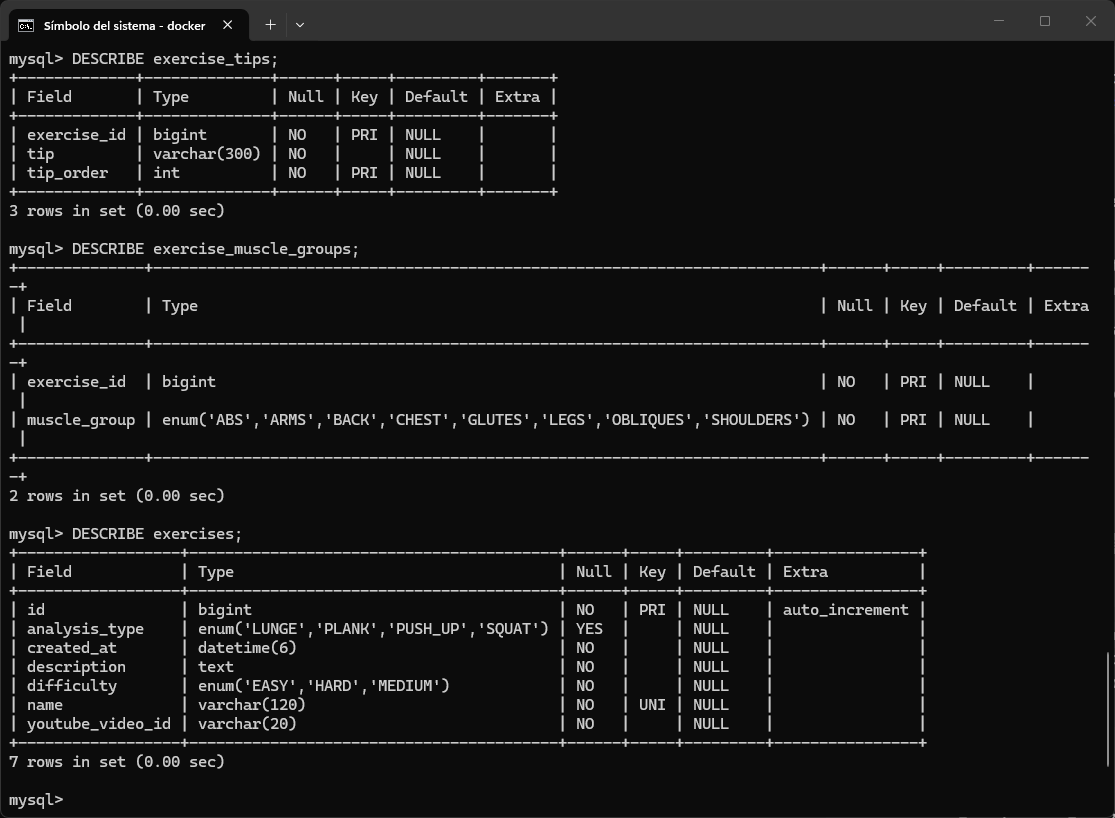
\includegraphics[width=0.85\textwidth]{img/tabla-exercise-creacion.png}
        \caption{Estructura de las tablas del catálogo generadas por Hibernate,
        verificada en MySQL.}
        \label{fig:tabla-exercise-creacion}
    \end{figure}

    El catálogo se puebla con un conjunto inicial de diez ejercicios. Para ello
    se descartó el uso de un guion SQL de inicialización por dos motivos. El
    primero es que los datos se reparten en tres tablas relacionadas, de modo
    que insertarlos mediante sentencias SQL obligaría a gestionar manualmente
    las claves ajenas. El segundo, más determinante, es que la estrategia de
    generación del esquema empleada ejecutaría dicho guion en cada arranque de
    la aplicación, duplicando los registros. En su lugar se ha implementado un
    componente que se ejecuta al iniciar la aplicación y que comprueba
    previamente si el catálogo contiene ya algún ejercicio; solo si está vacío
    procede a la inserción. El resultado es una carga idempotente: la
    aplicación puede arrancarse cuantas veces sea necesario sin alterar los
    datos existentes, como refleja la Figura~\ref{fig:carga-catalogo}.

    \begin{figure}[htbp]
        \centering
        \includegraphics[width=0.85\textwidth]{img/carga-catalogo.png}
        \caption{Trazas de la carga inicial del catálogo en el primer arranque
        y de su omisión en arranques posteriores.}
        \label{fig:carga-catalogo}
    \end{figure}

    \subsection{Consulta de filtrado y paginación}

    El listado de ejercicios admite tres criterios de filtrado independientes y
    opcionales, lo que plantea el problema de cómo construir una consulta que
    contemple todas sus combinaciones. Las soluciones habituales consisten en
    incorporar condiciones que comprueben si cada parámetro es nulo, o en
    construir la consulta dinámicamente concatenando fragmentos de texto. La
    primera produce consultas difíciles de leer y mantener; la segunda,
    consultas que no pueden validarse en tiempo de compilación.

    Se ha optado por un enfoque distinto: ausencia de filtro se traduce en
    filtrado por todos los valores posibles. Si el usuario no selecciona
    ninguna dificultad, la capa de servicio transmite las tres a la consulta;
    si no selecciona ningún grupo muscular, transmite los ocho; y si no
    introduce texto de búsqueda, transmite una cadena vacía, que al emplearse
    en una comparación por contenido coincide con todos los nombres. La
    consulta resultante es única, fija y sin ramificaciones, y devuelve
    exactamente el mismo resultado que las alternativas descritas.

    La consulta requiere además dos precauciones derivadas de la relación con
    los grupos musculares. La primera es la eliminación de duplicados: al
    combinar la tabla de ejercicios con la de grupos, un ejercicio que trabaje
    dos de los grupos seleccionados aparecería repetido en el resultado. La
    segunda afecta al recuento total de elementos, que debe declararse de forma
    explícita; la consulta de recuento que el marco de trabajo genera por
    defecto contabilizaría esas filas duplicadas y el número de resultados
    mostrado al usuario sería incorrecto.

    Por último, la capa de servicio impone un orden por nombre cuando la
    petición no especifica otro. En una consulta paginada el orden no es una
    cuestión estética: sin una ordenación estable, la base de datos no
    garantiza que dos peticiones consecutivas devuelvan las filas en la misma
    secuencia, de modo que un mismo ejercicio podría aparecer en dos páginas
    distintas o no aparecer en ninguna.

    \subsection{Objetos de transferencia y etiquetas de presentación}

    La API no expone las entidades directamente, sino objetos de transferencia
    específicos para cada vista: uno reducido para las tarjetas del listado y
    otro completo, con la descripción y los consejos, para el detalle. Ambos se
    construyen mediante una clase de conversión que centraliza también la
    composición de la dirección de la miniatura a partir del identificador del
    vídeo.

    Los valores enumerados no se transmiten como una cadena simple, sino como
    un par formado por el identificador técnico y la etiqueta en castellano.
    Así, el grupo muscular de los glúteos viaja al cliente acompañado del texto
    que debe mostrarse. El cliente utiliza el identificador para construir las
    peticiones de filtrado y la etiqueta para representarlo en pantalla, sin
    necesidad de mantener su propia tabla de traducciones. Esta decisión evita
    que un cambio en los textos visibles, o la incorporación de un nuevo grupo
    muscular, obligue a modificar de forma coordinada el servidor y el cliente.

    Los objetos de transferencia incluyen ya los campos correspondientes a la
    valoración media, el número de valoraciones y la condición de favorito, que
    en esta fase se devuelven con valores neutros. Anticiparlos permite que los
    componentes de la interfaz queden construidos en su forma definitiva y que
    la incorporación de dichas funcionalidades, prevista en un incremento
    posterior, no requiera modificar el contrato de la API ni los componentes
    ya desarrollados.

    \subsection{Vista de catálogo}

    En el cliente, el catálogo se apoya en dos componentes reutilizables: la
    tarjeta de ejercicio y la barra de filtros, ambos concebidos para emplearse
    también en la vista de ejercicios favoritos. La página se limita a
    coordinarlos y a gestionar la comunicación con la API. La
    Figura~\ref{fig:catalogo-implementado} muestra el resultado.

    \begin{figure}[htbp]
        \centering
        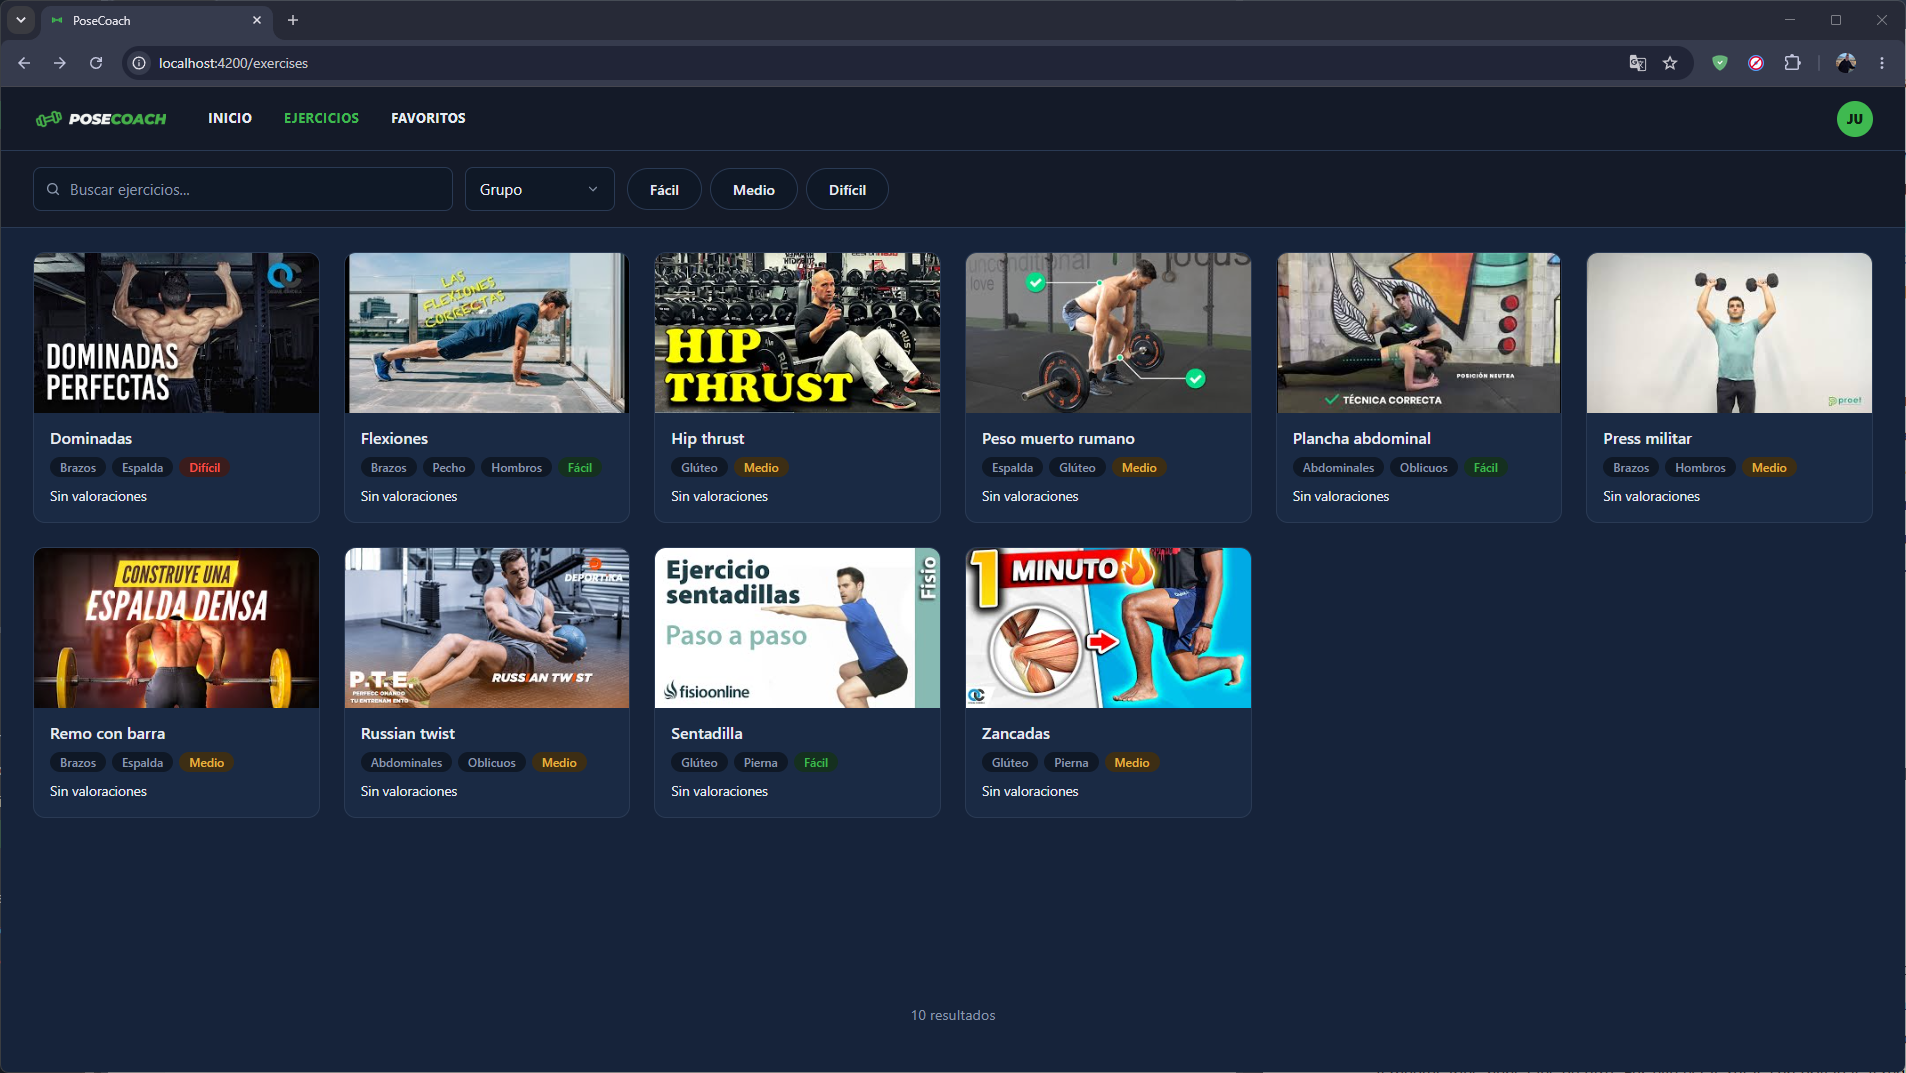
\includegraphics[width=\textwidth]{img/catalogo-implementado.png}
        \caption{Vista de catálogo con el conjunto completo de ejercicios.}
        \label{fig:catalogo-implementado}
    \end{figure}

    El comportamiento de la búsqueda por texto requirió dos ajustes en el
    tratamiento de las peticiones. El primero es la introducción de un retardo
    entre la última pulsación de tecla y el envío de la consulta: sin él, cada
    carácter escrito generaría una petición al servidor, de modo que buscar una
    palabra de diez letras produciría diez consultas de las que solo la última
    resulta útil. El segundo es la cancelación de las peticiones que quedan
    obsoletas. Cuando el usuario modifica los criterios antes de que se haya
    recibido la respuesta anterior, ambas peticiones quedan en curso
    simultáneamente y nada garantiza que respondan en el mismo orden en que se
    enviaron; si la más antigua llegase en último lugar, sobrescribiría unos
    resultados más recientes y la interfaz mostraría un listado que no
    corresponde a los filtros seleccionados. El operador empleado descarta
    automáticamente la petición en curso al recibir un criterio nuevo.

    Los criterios de filtrado se reflejan además en los parámetros de consulta
    de la dirección del navegador. Esto proporciona tres ventajas: la búsqueda
    puede compartirse mediante un enlace, se conserva al recargar la página y,
    sobre todo, sobrevive a la navegación hacia el detalle de un ejercicio y de
    vuelta al listado. Los valores recibidos por esta vía se contrastan con los
    admitidos antes de emplearse, de modo que una dirección manipulada
    manualmente no llega a generar una petición no válida al servidor. La
    Figura~\ref{fig:catalogo-filtrado} muestra el catálogo con varios filtros
    activos y su reflejo en la dirección.

    \begin{figure}[htbp]
        \centering
        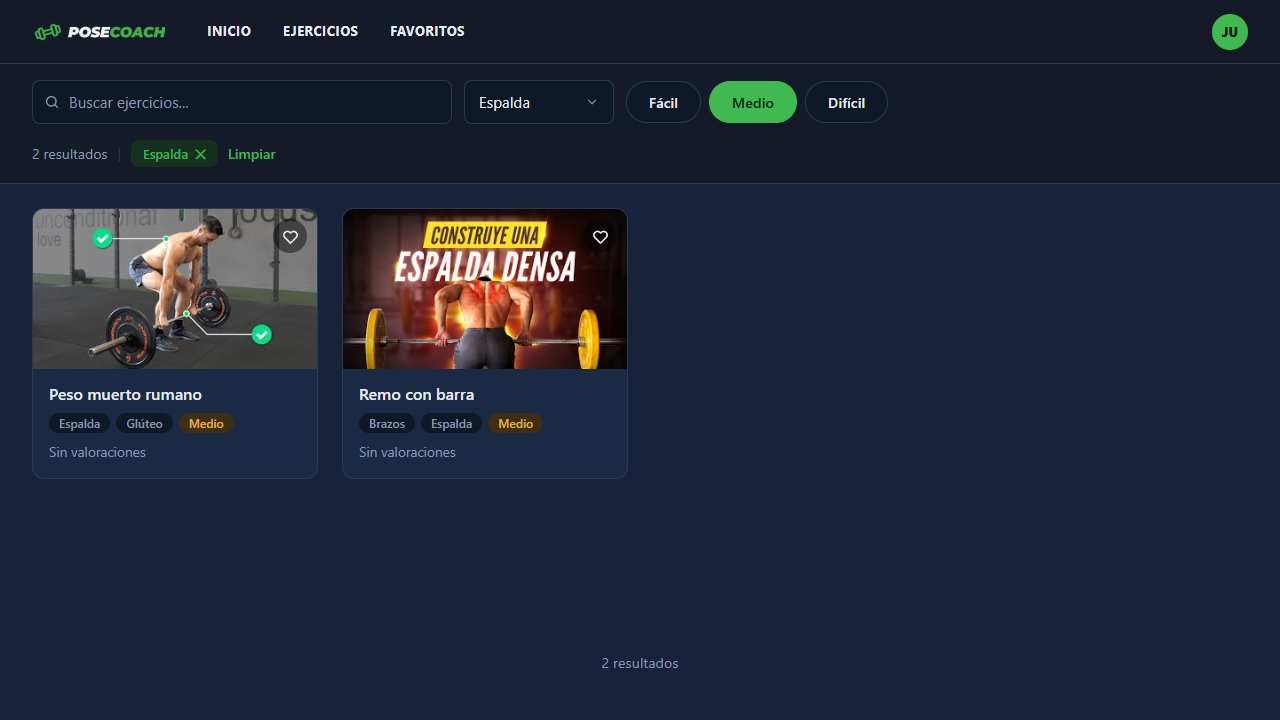
\includegraphics[width=\textwidth]{img/catalogo-filtrado.png}
        \caption{Catálogo filtrado por grupo muscular y dificultad, con los
        criterios reflejados en la dirección del navegador.}
        \label{fig:catalogo-filtrado}
    \end{figure}

    \subsection{Vista de detalle y vídeo embebido}

    La vista de detalle se estructura en las tres pestañas descritas en el
    capítulo de diseño, de las cuales solo la de información corresponde a este
    incremento. La pestaña de análisis postural se muestra únicamente en
    aquellos ejercicios cuyo atributo \texttt{analysisType} tiene valor, lo que
    permite verificar desde ya el comportamiento condicional de la interfaz.

    La Figura~\ref{fig:detalle-sin-analisis} muestra el detalle de un ejercicio
    sin analizador asociado, en el que la pestaña correspondiente no aparece,
    en contraste con la Figura~\ref{fig:detalle-implementado}.

    \begin{figure}[htbp]
        \centering
        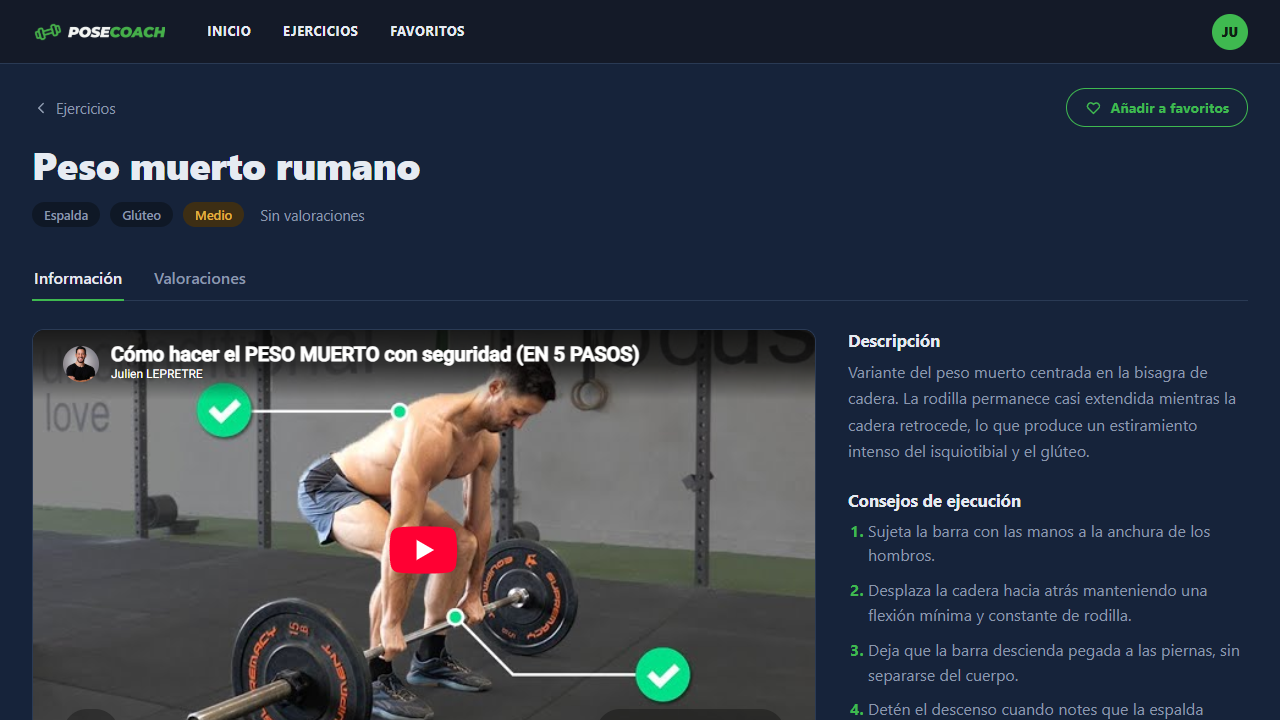
\includegraphics[width=\textwidth]{img/detalle-sin-analisis.png}
        \caption{Detalle de un ejercicio sin analizador postural asociado,
        donde la pestaña de análisis no se muestra.}
        \label{fig:detalle-sin-analisis}
    \end{figure}

    La reproducción del vídeo se realiza mediante un marco embebido. Angular
    bloquea por defecto la asignación dinámica de direcciones a este tipo de
    elementos, al tratarse de un vector habitual de inyección de código, por lo
    que la dirección debe autorizarse de forma explícita. Dicha autorización es
    segura en este caso porque el identificador del vídeo no procede de una
    entrada del usuario, sino de la base de datos, y se inserta en una
    dirección de dominio fijo; la valoración sería distinta si el identificador
    pudiera introducirse desde un formulario.

    La dirección empleada corresponde al dominio de reproducción con protección
    de privacidad reforzada que ofrece la plataforma, que no instala cookies de
    seguimiento hasta que el usuario inicia la reproducción. Esta elección es
    coherente con el requisito no funcional RNF-02, que establece la
    preservación de la privacidad del usuario como criterio de diseño del
    sistema. La Figura~\ref{fig:detalle-implementado} muestra la vista
    resultante.

    \begin{figure}[htbp]
        \centering
        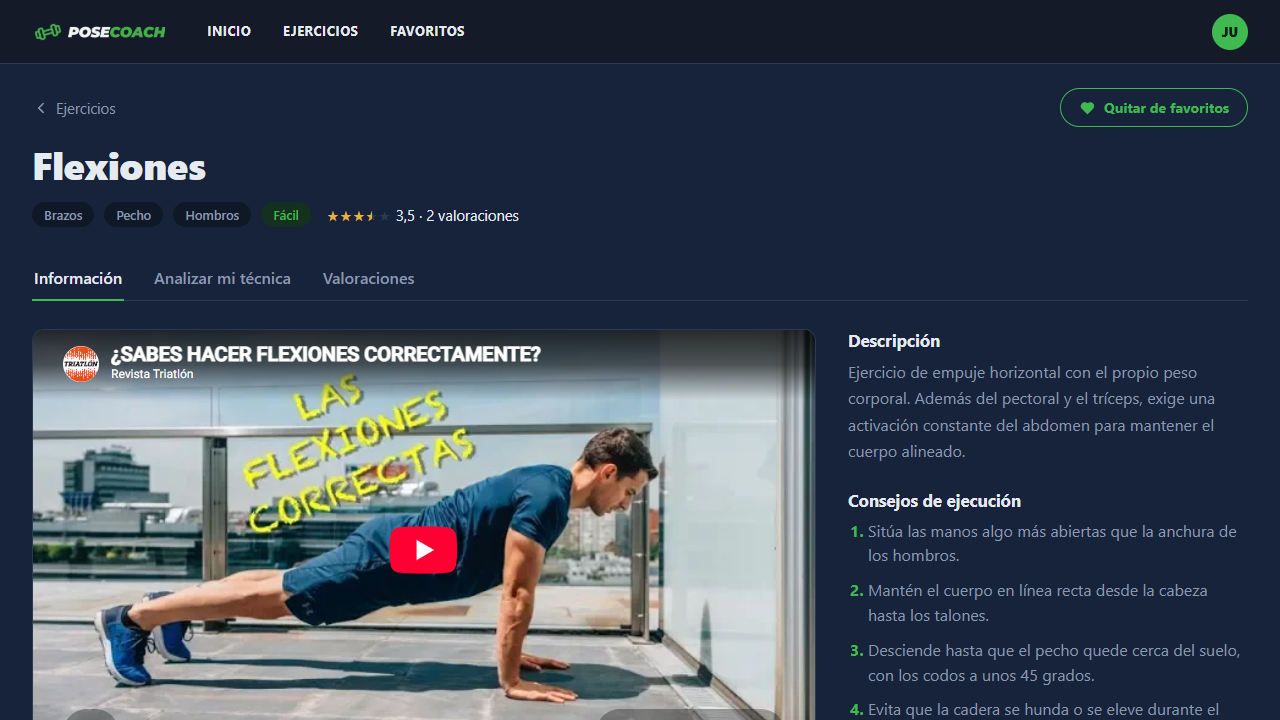
\includegraphics[width=\textwidth]{img/detalle-implementado.png}
        \caption{Vista de detalle de un ejercicio, con el vídeo demostrativo,
        la descripción y los consejos de ejecución.}
        \label{fig:detalle-implementado}
    \end{figure}

    \section{Valoraciones y favoritos}

    El tercer módulo implementado da soporte a los requisitos RF-05, RF-06 y
    RF-07, e introduce una diferencia cualitativa respecto a los anteriores:
    hasta ahora los datos eran o bien propios de un usuario, o bien comunes a
    todos, mientras que aquí cada dato pertenece a un usuario concreto pero se
    muestra a los demás. Esta condición atraviesa todo el módulo y explica
    buena parte de las decisiones que se detallan a continuación.

    \subsection{Reestructuración de la organización en paquetes}

    Antes de abordar la funcionalidad se acometió una reorganización del
    código del servidor. Los dos módulos anteriores habían dado lugar a dos
    criterios de organización simultáneos: la mayor parte de las clases se
    agrupaban por capa arquitectónica (modelo, repositorio, servicio,
    controlador), pero las del catálogo se habían agrupado por funcionalidad en
    un paquete propio que reunía la entidad, su conversor a objetos de
    transferencia y su componente de carga inicial, es decir, tres clases de
    tres capas distintas.

    Ambos criterios son legítimos y de uso extendido, pero su coexistencia no
    lo es: obliga a conocer el historial del proyecto para saber dónde buscar
    una clase. Se optó por unificar en la organización por capas, que era la
    predominante y la descrita en los capítulos previos, distribuyendo las
    clases del catálogo entre los paquetes correspondientes y creando dos
    paquetes adicionales para los conversores y para las excepciones de
    dominio, que hasta entonces convivían con los servicios y los
    controladores. La Tabla~\ref{tab:paquetes} recoge la estructura
    resultante.

    \begin{table}[htbp]
        \centering
        \begin{tabular}{l p{8.5cm}}
            \toprule
            \textbf{Paquete} & \textbf{Contenido} \\
            \midrule
            model      & Entidades JPA y tipos enumerados del dominio \\
            repository & Interfaces de acceso a datos \\
            service    & Lógica de negocio \\
            controller & Puntos de entrada de la API REST \\
            dto        & Objetos de transferencia y proyecciones \\
            mapper     & Conversión entre entidades y objetos de transferencia \\
            exception  & Excepciones de dominio y manejador global \\
            security   & Componentes de autenticación basada en tokens \\
            config     & Configuración y carga inicial de datos \\
            util       & Utilidades transversales \\
            \bottomrule
        \end{tabular}
        \caption{Organización en paquetes del servidor tras la
        reestructuración.}
        \label{tab:paquetes}
    \end{table}

    La reestructuración se realizó mediante las herramientas de refactorización
    automática del entorno de desarrollo, que actualizan las referencias
    afectadas, y se registró en un cambio independiente del resto del
    incremento. Esta separación no es accesoria: permite comprobar que la
    modificación se limita a declaraciones de paquete e importaciones, sin
    alterar una sola línea de lógica, lo que constituye la definición misma de
    una refactorización. Conviene subrayar además que el cambio no afecta a la
    base de datos, ya que el nombre de cada tabla lo fija la anotación
    \texttt{@Table} de la entidad y no su ubicación en el código.

    \subsection{Modelo de dominio y persistencia}

    Las entidades \texttt{Review} y \texttt{Favorite}, cuyos atributos se
    recogieron en las Tablas~\ref{tab:entidad-review}
    y~\ref{tab:entidad-favorite}, se mapean a las tablas \texttt{reviews} y
    \texttt{favorites}. Ambas se relacionan con \texttt{User} y con
    \texttt{Exercise} mediante asociaciones de muchos a uno con carga diferida,
    y ninguna de las dos entidades del otro extremo declara la colección
    inversa. Esta omisión es deliberada: una colección de valoraciones en
    \texttt{Exercise} induciría a recorrerla para calcular la media, con el
    coste de recuperar de la base de datos todas las valoraciones de un
    ejercicio cada vez que se consulta su ficha.

    La restricción que impone las reglas RN-01 y RN-05 se declara mediante el
    atributo \texttt{uniqueConstraints} de la anotación \texttt{@Table}, que
    genera en cada tabla un índice único sobre el par de claves ajenas. Es
    importante notar que esta garantía no sustituye a la comprobación que
    realiza el servicio, sino que la respalda: la comprobación previa permite
    responder con un mensaje comprensible en el caso habitual, mientras que la
    restricción de la tabla cubre el escenario en que dos peticiones
    simultáneas superen ambas dicha comprobación antes de que ninguna haya
    guardado.

    Las marcas temporales se asignan mediante métodos anotados con
    \texttt{@PrePersist} y \texttt{@PreUpdate}, siguiendo el mecanismo ya
    empleado en las entidades anteriores. Durante la implementación se detectó
    que las entidades existentes no eran consistentes en este punto: unas
    fijaban la zona horaria de forma explícita y otras empleaban la del sistema
    anfitrión, lo que haría incomparables las fechas de un mismo sistema al
    desplegarse en máquinas distintas. Se centralizó por ello la obtención de
    la marca temporal en una clase de utilidad común a las cuatro entidades.

    Tras el primer arranque se verificó en MySQL la creación de ambas tablas
    con sus columnas, claves ajenas y restricciones de unicidad
    (Figura~\ref{fig:tablas-social-creacion}), siguiendo el mismo procedimiento
    aplicado en los incrementos anteriores.

    \begin{figure}[htbp]
        \centering
        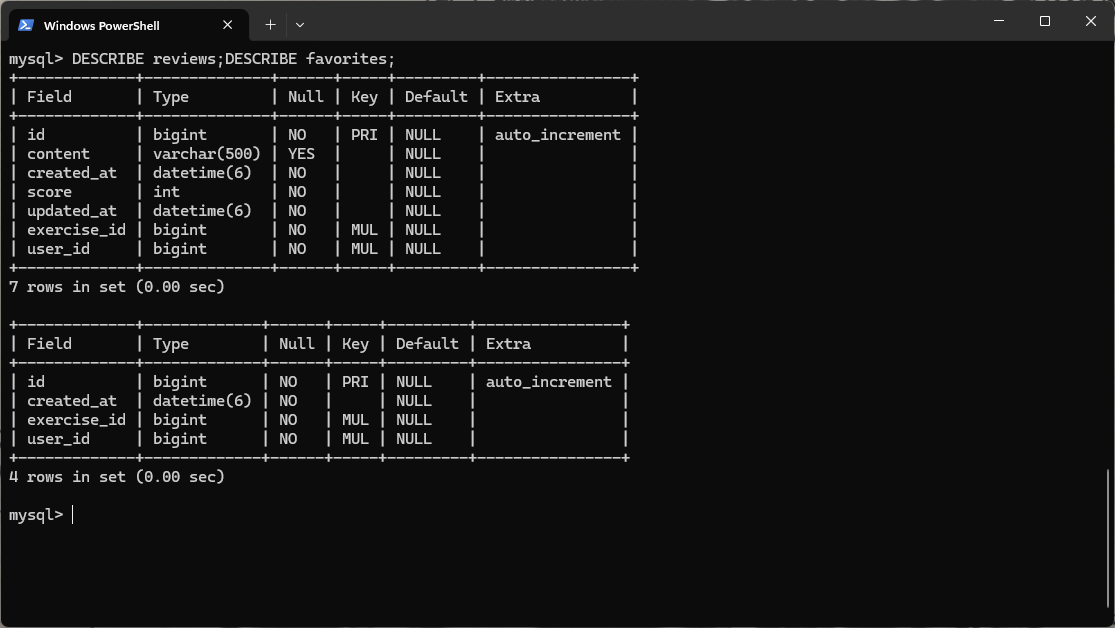
\includegraphics[width=0.85\textwidth]{img/tablas-social-creacion.png}
        \caption{Estructura de las tablas \texttt{reviews} y \texttt{favorites}
        generadas por Hibernate, verificada en MySQL.}
        \label{fig:tablas-social-creacion}
    \end{figure}

    \subsection{Registro y modificación de la valoración}

    El registro de una valoración se resuelve con un único procedimiento que
    localiza la valoración del usuario sobre el ejercicio y, si existe,
    reutiliza la fila modificando sus valores, mientras que si no existe crea
    una nueva. No hay por tanto ninguna comprobación explícita que rechace una
    segunda valoración: la regla RN-01 se satisface porque el código no dispone
    de ninguna vía para crearla. La consecuencia práctica es que publicar una
    valoración por primera vez y editar una ya existente son literalmente la
    misma operación, lo que permitió incorporar la edición desde la interfaz
    sin escribir código adicional en el servidor.

    Este planteamiento se apoya en el diseño de la API descrito en la
    Sección~\ref{sec:api-social}: al identificarse el recurso como la
    valoración propia del usuario sobre un ejercicio, y no mediante un
    identificador de valoración, la operación resulta idempotente y la
    identidad del autor procede necesariamente del token.

    El comentario recibido se normaliza antes de persistirse: una cadena
    compuesta únicamente por espacios, o vacía, se almacena como valor nulo. La
    razón es que el formulario de la interfaz envía una cadena vacía cuando el
    usuario se limita a seleccionar estrellas, y almacenarla tal cual haría
    aparecer una entrada sin texto en el listado de comentarios. Con esta
    normalización, la regla RN-03 se traduce en una distinción inequívoca entre
    valoración con comentario y valoración sin él.

    \subsection{Cálculo de la valoración media y de la distribución}

    Conforme a la regla RN-06, la valoración media no se almacena, de modo que
    debe obtenerse en cada consulta. Resolverlo de la manera más directa
    ---preguntar por la media de cada ejercicio mientras se recorre la página
    de resultados--- reproduciría el problema \textit{N+1} ya descrito en el
    catálogo, con una consulta adicional por cada tarjeta mostrada. La solución
    empleada allí, la anotación \texttt{@BatchSize}, no es aplicable en este
    caso, ya que no se trata de cargar una colección de la propia entidad sino
    de agregar datos residentes en otra tabla.

    Se optó por una consulta agregada única que recibe los identificadores de
    todos los ejercicios de la página y devuelve, agrupados por ejercicio, su
    media y su número de valoraciones. El servicio indexa el resultado en
    memoria y lo combina con cada ejercicio al construir el objeto de
    transferencia. El coste del listado pasa así a ser un número fijo de
    consultas con independencia del número de tarjetas.

    Este planteamiento obliga a contemplar dos situaciones que la agregación
    deja implícitas. La primera es que una cláusula \texttt{GROUP BY} solo
    devuelve grupos existentes, de modo que un ejercicio sin ninguna valoración
    no aparece en el resultado; el servicio interpreta su ausencia como media y
    recuento nulos, que es la representación correcta y la que la interfaz
    traduce en la leyenda «Sin valoraciones». La segunda es que una cláusula
    \texttt{IN} con una lista vacía no constituye SQL válido, situación que se
    produce precisamente cuando un filtro no arroja resultados, por lo que el
    servicio evita lanzar la consulta en ese caso.

    La distribución de puntuaciones que muestra la vista de detalle se obtiene
    con una consulta análoga, agrupada esta vez por puntuación. Presenta el
    mismo fenómeno a mayor escala: los niveles que ninguna persona ha
    seleccionado no figuran en el resultado, mientras que la interfaz debe
    representar siempre las cinco barras. El servicio completa por ello los
    niveles ausentes con valor cero antes de devolver el resultado.

    Una vez obtenida la distribución, la media del ejercicio se deriva de ella
    como media ponderada en lugar de solicitarse a la base de datos mediante
    una segunda consulta. Además de ahorrar un acceso, este cálculo garantiza
    que el valor mostrado y las barras representadas procedan del mismo dato y
    no puedan contradecirse. El resultado se redondea a un decimal en el
    servidor, evitando que la API publique valores con una precisión carente de
    significado.

    \subsection{Listado de comentarios}

    El listado de comentarios de un ejercicio se obtiene mediante una consulta
    paginada sobre la tabla de valoraciones que aplica tres condiciones. La
    primera descarta las valoraciones sin texto, que computan en la media y en
    la distribución pero no constituyen comentarios. La segunda excluye la
    valoración del propio usuario, dado que la interfaz la presenta de forma
    destacada al inicio; incluirla en el listado la duplicaría y, al estar
    paginado, alteraría además el recuento de elementos pendientes. La tercera
    ordena los resultados por fecha de publicación y no por fecha de
    modificación, de manera que corregir un comentario antiguo no lo desplace
    al primer puesto.

    La consulta recupera de forma anticipada el autor de cada comentario
    mediante una reunión explícita. Sin ella, la construcción del objeto de
    transferencia, que necesita el nombre de usuario, provocaría una consulta
    adicional por cada comentario de la página: es la tercera manifestación del
    problema \textit{N+1} en este incremento, y la tercera técnica distinta
    empleada para resolverlo, lo que ilustra que no existe una solución única
    sino que depende de la naturaleza del dato que falta.

    \subsection{Marcado de ejercicios favoritos}

    Las dos operaciones sobre el favorito se implementan de forma idempotente,
    conforme al diseño de la API: marcar un ejercicio ya marcado no produce
    efecto alguno ni se considera un error, y lo mismo ocurre al retirar uno
    que no lo estaba. El listado de favoritos se obtiene mediante una consulta
    que reúne los ejercicios con sus marcas y los ordena por la fecha en que se
    guardaron, atributo cuya existencia justifica que la relación se modelase
    como entidad.

    Para determinar qué ejercicios de una página son favoritos del usuario se
    aplica la misma estrategia empleada con las valoraciones: una única
    consulta que devuelve, de entre los identificadores de la página,
    únicamente los marcados. Devolver identificadores y no entidades resulta
    suficiente, ya que la interfaz solo necesita saber si cada ejercicio
    pertenece o no al conjunto.

    La consecuencia de haber resuelto ambos datos de forma agregada es que el
    listado del catálogo, que muestra por cada tarjeta información procedente
    de tres tablas distintas, se resuelve con un número constante de consultas.
    El listado de favoritos reutiliza íntegramente este mecanismo, de modo que
    no constituye una vista nueva sino el mismo listado con un origen de datos
    distinto.

    \subsection{Control de acceso a las operaciones sociales}

    Ninguna de las clases de este módulo contiene comprobaciones de
    autenticación. La protección procede de la configuración de Spring
    Security establecida en el primer incremento, que declara públicas
    únicamente las rutas de autenticación y exige un token válido en cualquier
    otra, por lo que las rutas nuevas quedaron protegidas sin necesidad de
    modificarla. Una petición sin token válido no llega a alcanzar el
    controlador.

    La identidad del usuario se obtiene siempre del contexto de seguridad, que
    el filtro de autenticación establece a partir del token verificado, y nunca
    del cuerpo de la petición ni de la ruta. Combinado con el diseño de la API,
    esto produce una propiedad relevante: dado que ninguna ruta acepta el
    identificador de una valoración, sino el del ejercicio, la búsqueda se
    realiza siempre por la pareja formada por el ejercicio y el usuario
    autenticado, de modo que solo puede localizar valoraciones propias. La
    regla RN-04 no se sostiene por tanto sobre una comprobación que pudiera
    omitirse en una operación futura, sino sobre la imposibilidad de expresar
    la petición.

    Los objetos de transferencia de entrada refuerzan este planteamiento al
    declarar exclusivamente los campos que el cliente puede decidir. Una
    petición que incluyese un nombre de usuario en el cuerpo no produciría
    error alguno, sencillamente sería ignorada, ya que ningún campo del objeto
    receptor le corresponde.

    Un último aspecto de seguridad afecta al cliente. El contenido de los
    comentarios lo redacta un usuario y se muestra a los demás, lo que
    constituye el escenario propio de un ataque de \textit{cross-site
    scripting}. La interfaz representa ese contenido mediante interpolación,
    mecanismo que en Angular escapa el texto de forma predeterminada, de manera
    que un comentario que incluyese etiquetas HTML se muestra literalmente en
    lugar de interpretarse. Se evita deliberadamente el enlace a la propiedad
    \texttt{innerHTML}, que sí interpretaría el contenido.

    \subsection{Componentes reutilizables de la interfaz}

    La representación de una puntuación mediante estrellas aparece en tres
    contextos distintos ---la tarjeta del catálogo, la cabecera del detalle y
    cada comentario---, además del formulario de valoración, donde debe admitir
    interacción. Se implementó por ello como un componente propio con tres
    modos de funcionamiento (lectura, selección y selección bloqueada) y tres
    tamaños, que sustituyó a las representaciones parciales que los incrementos
    anteriores habían resuelto con un carácter suelto.

    El componente debe representar valores decimales, dado que la valoración
    media rara vez es un número entero. En lugar de recurrir a un icono de
    media estrella, que solo permitiría representar mitades, se superponen dos
    filas de cinco estrellas: una inferior en color neutro y otra superior en
    color de acento cuya anchura visible se recorta en proporción al valor. Una
    media de 4,2 se traduce así en un 84\% de anchura, y el navegador secciona
    la quinta estrella por el punto exacto, con independencia del tamaño de
    representación.

    Las fechas de los comentarios se muestran en términos relativos a partir de
    la marca temporal recibida. La conversión se resuelve con la interfaz de
    internacionalización que proporciona el propio navegador, evitando incluir
    una biblioteca adicional únicamente para este fin y obteniendo los textos
    en castellano sin necesidad de mantener traducciones propias. Conviene
    señalar una limitación conocida: la transformación se evalúa una sola vez
    por valor, de modo que el texto no se actualiza mientras la vista permanece
    abierta, comportamiento aceptable en una pantalla de consulta.

    \subsection{La pestaña de valoraciones}

    La pestaña de valoraciones requiere dos peticiones: el resumen, que aporta
    la media, la distribución y la valoración propia, y la primera página de
    comentarios. Ambas se lanzan únicamente al abrir la pestaña, de modo que un
    usuario que consulte la descripción de un ejercicio y abandone la vista no
    incurre en su coste, y se emiten de forma simultánea, ya que ninguna
    depende del resultado de la otra; la vista se compone cuando ambas han
    respondido.

    Tras publicar, modificar o eliminar una valoración se recargan ambas
    peticiones en lugar de actualizar el estado local con la respuesta
    recibida. Aunque esta segunda opción evitaría dos accesos, la operación
    afecta simultáneamente a la media, a la distribución, al recuento y a la
    composición del listado, dado que el comentario propio se excluye de este y
    pasa a mostrarse de forma destacada. Reproducir en el cliente todas esas
    transformaciones supondría duplicar reglas que ya residen en el servidor y
    abriría la puerta a discrepancias entre lo mostrado y lo almacenado.

    La cabecera de la vista, que muestra también la media y el recuento,
    procede sin embargo de una petición distinta realizada al cargar el
    ejercicio. Para no repetirla completa se actualizan únicamente esos dos
    valores con los que devuelve el resumen. Por último, el estado de la
    pestaña se reinicia al navegar de un ejercicio a otro, ya que el marco de
    trabajo reutiliza la misma instancia del componente y, sin ese reinicio, se
    mostrarían momentáneamente las valoraciones del ejercicio anterior.

    Durante las pruebas de la interfaz se detectó un defecto que ilustra el
    valor de recorrer la aplicación completa y no solo verificar los puntos de
    entrada de la API por separado. Las acciones de edición y eliminación se
    habían situado inicialmente junto al comentario propio destacado, ubicación
    razonable mientras se supone que toda valoración lleva texto. Un usuario
    que puntuase sin comentar no generaba comentario alguno y, en consecuencia,
    quedaba sin ninguna forma de modificar o retirar su valoración, con el
    formulario bloqueado por tenerla ya publicada. La corrección consistió en
    trasladar ambas acciones al propio formulario, que está siempre presente, y
    resultó además más coherente con el alcance real de la eliminación, que
    afecta a la valoración completa y no solo al comentario.

    \subsection{Un efecto colateral entre la reactividad y el DOM}

    La incorporación del botón de favorito a la vista de detalle produjo un
    comportamiento inesperado: tras marcarlo o desmarcarlo, el control de
    retroceso del navegador exigía dos pulsaciones para abandonar la vista, y
    el vídeo embebido se reiniciaba.

    El origen resultó estar tres pasos por delante del síntoma. Al cambiar la
    condición de favorito se sustituye el objeto que representa el ejercicio,
    tal como exige el modelo de reactividad basado en señales, que detecta los
    cambios comparando referencias. Esa sustitución provocaba el recálculo del
    valor derivado que compone la dirección del vídeo, la cual debe declararse
    explícitamente como segura para poder emplearse en un marco flotante; dicha
    declaración devuelve una instancia distinta en cada invocación, aunque el
    identificador del vídeo sea idéntico. El enlace de la propiedad
    correspondiente detectaba por tanto un valor nuevo y reasignaba el origen
    del marco, que volvía a cargarse. Y una navegación dentro de un marco
    flotante añade una entrada al historial de la pestaña, de modo que la
    primera pulsación de retroceso se consumía deshaciendo esa recarga.

    La corrección consistió en interponer un valor derivado intermedio que
    expone únicamente el identificador del vídeo. Al tratarse de una cadena de
    texto, su comparación por igualdad determina que no ha cambiado y detiene
    la propagación antes de alcanzar el cálculo de la dirección, que ya no se
    reevalúa. Es un patrón de aplicación general: cuando un cálculo costoso o
    con efectos colaterales depende de un objeto que se sustituye por motivos
    ajenos a él, conviene intercalar un valor derivado con el dato mínimo del
    que realmente depende.

    \subsection{Consolidación técnica al cierre del incremento}

    Antes de dar por concluido el incremento se abordó un conjunto de mejoras
    de coherencia interna acumuladas durante su desarrollo, registradas como
    tareas específicas a medida que se detectaban. Este proceder responde a un
    criterio deliberado: interrumpir la implementación de una funcionalidad
    para corregir cada detalle fragmenta el trabajo, mientras que posponerlos
    indefinidamente los convierte en deuda técnica. Las principales
    actuaciones fueron las siguientes.

    En el servidor se unificó la obtención de las marcas temporales en una
    utilidad común, corrigiendo la inconsistencia de zona horaria ya descrita;
    se homogeneizó el formato de las respuestas de error conforme a lo expuesto
    en el capítulo de diseño, lo que exigió actualizar los cuatro puntos del
    cliente que interpretaban el formato anterior; se sustituyeron las
    recuperaciones del usuario autenticado que finalizaban con una excepción
    genérica, y que habrían producido un error interno sin mensaje, por una
    excepción propia traducida a \texttt{401 Unauthorized}, código que describe
    con mayor precisión la situación, un token que identifica a un usuario
    inexistente, y que el cliente ya interpreta cerrando la sesión; y se
    uniformó el estilo de inyección de dependencias en todos los servicios.

    En el cliente se extrajo a un fichero de configuración la dirección base de
    la API, replicada hasta entonces en cada servicio; se incorporaron al
    sistema de diseño las clases repetidas en varias hojas de estilo; se
    corrigió el uso de los colores de superficie, que en el módulo nuevo se
    habían aplicado en orden inverso al establecido; y se registró la
    configuración regional española, sin la cual la valoración media se
    representaba con separador decimal anglosajón.

    No todas las incidencias registradas se resolvieron. Se descartó
    conscientemente extraer a una utilidad una función auxiliar empleada
    únicamente en dos lugares, incluir el identificador del usuario en el token
    para ahorrar una consulta por petición, paginar el listado de favoritos y
    reforzar el mecanismo de retroceso frente a interacciones del usuario con
    el reproductor de vídeo. En los cuatro casos el coste de la modificación
    excedía al beneficio con el volumen de datos previsto, y su registro
    explícito permite distinguir entre deuda técnica asumida de forma
    razonada y descuido.


    \section{Módulo de corrección postural}

    \subsection{Estimación de pose con MediaPipe}

    \subsection{Cálculo de métricas: ángulos articulares y alineaciones}

    \subsection{Feedback y puntuación global}


    \section{Contenerización con Docker}


% ─────────────────────── Capítulo 7 ──────────────────────────────────


    \chapter{Pruebas y validación}
    \label{cap:pruebas}


    \section{Pruebas funcionales}
    Para validar el endpoint de registro se realizaron pruebas funcionales con
    la herramienta Postman, comprobando tanto el caso correcto como los casos de
    error. La Figura~\ref{fig:postman-201} muestra un registro exitoso
    (\texttt{201 Created}); la Figura~\ref{fig:postman-409}, el rechazo de un
    usuario duplicado (\texttt{409 Conflict}); y la Figura~\ref{fig:postman-400},
    el rechazo de un correo con formato inválido (\texttt{400 Bad Request}).

    \begin{figure}[htbp]
        \centering
        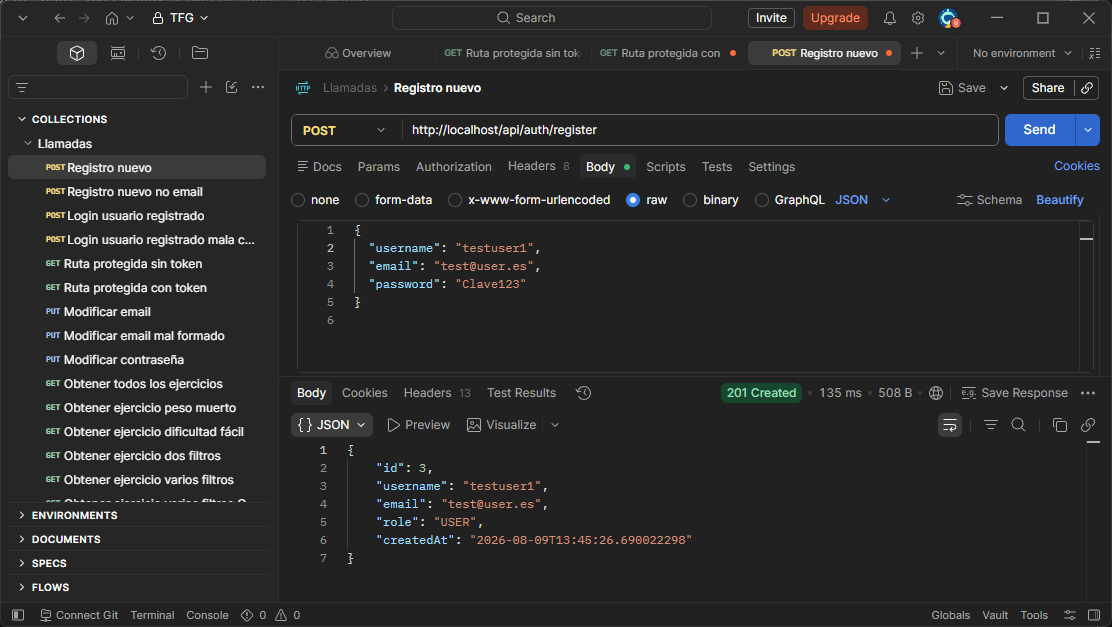
\includegraphics[width=0.9\textwidth]{img/postman-201.png}
        \caption{Registro correcto de un usuario: respuesta \texttt{201 Created}.}
        \label{fig:postman-201}
    \end{figure}

    \begin{figure}[htbp]
        \centering
        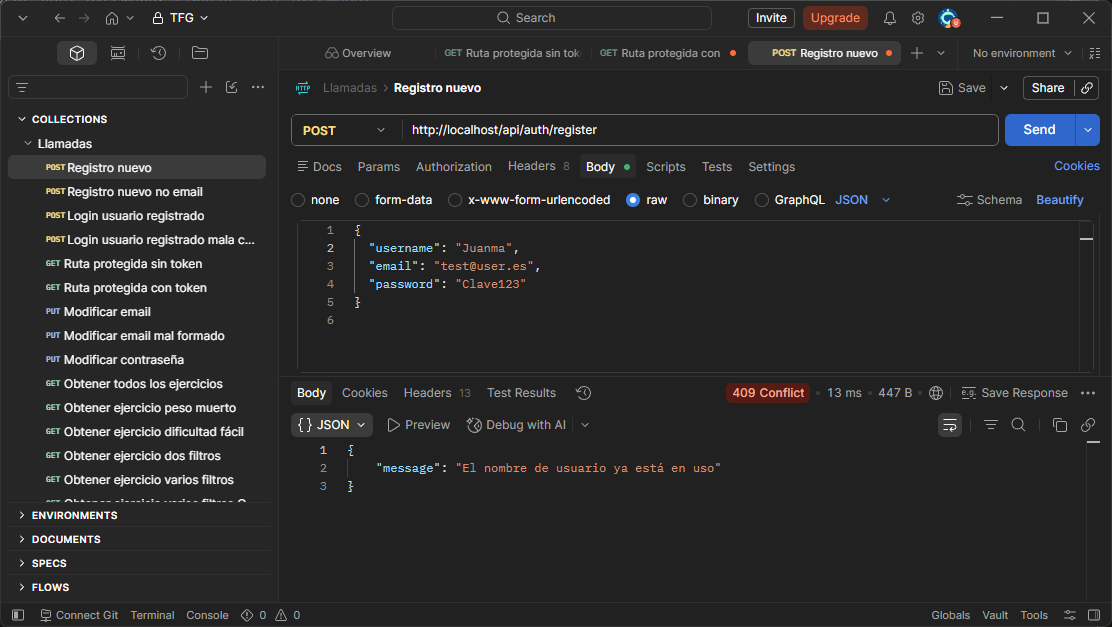
\includegraphics[width=0.9\textwidth]{img/postman-409.png}
        \caption{Intento de registro con un usuario ya existente: respuesta
        \texttt{409 Conflict}.}
        \label{fig:postman-409}
    \end{figure}

    \begin{figure}[htbp]
        \centering
        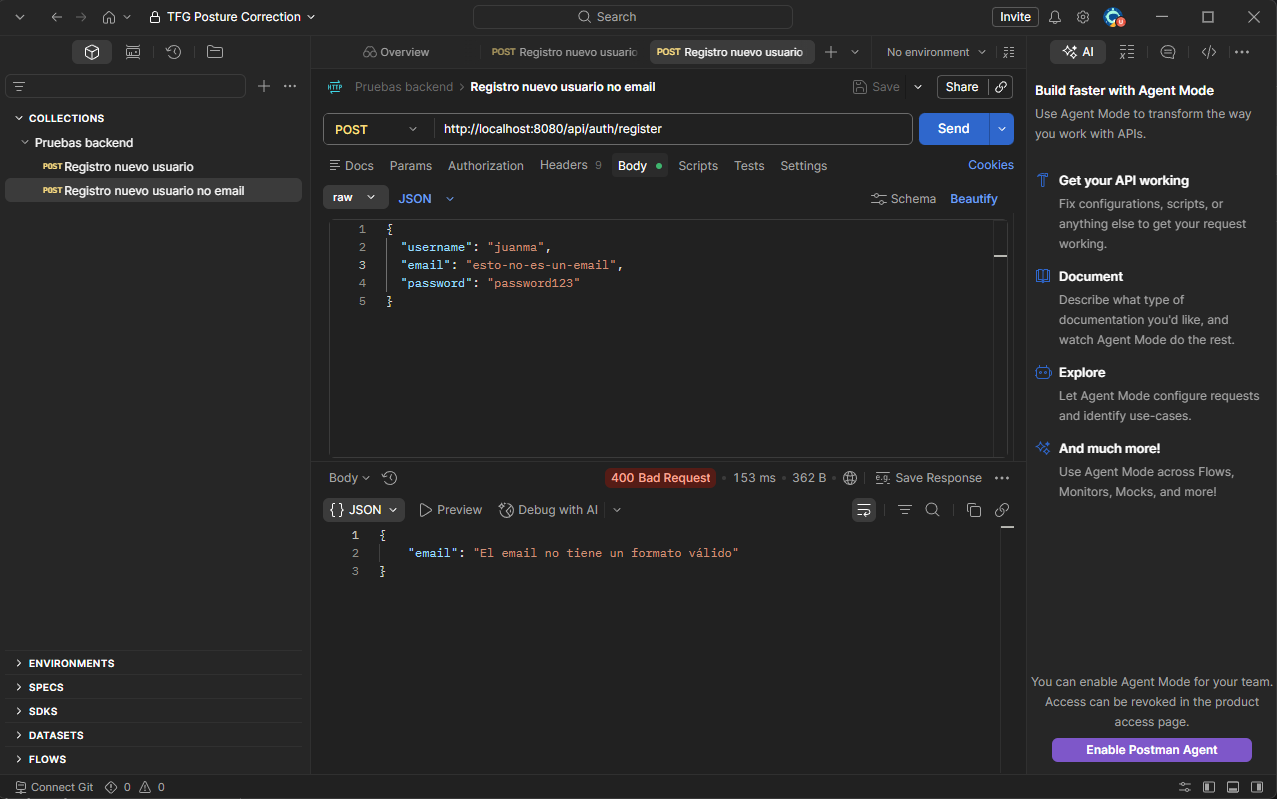
\includegraphics[width=0.9\textwidth]{img/postman-400.png}
        \caption{Registro con un correo inválido: respuesta \texttt{400 Bad
        Request} con el mensaje de validación.}
        \label{fig:postman-400}
    \end{figure}

    \section{Pruebas de integración de la interfaz}

    Una vez implementada la interfaz del módulo de usuarios, se realizó una
    prueba manual del flujo completo con el objetivo de verificar la correcta
    integración entre cliente y servidor. A diferencia de las pruebas
    anteriores, centradas en los endpoints de forma aislada, estas comprueban el
    recorrido real de un usuario a través de la aplicación. La
    Tabla~\ref{tab:pruebas-flujo} recoge los casos verificados y el resultado
    esperado en cada uno.

    \begin{table}[htbp]
        \centering
        \small
        \begin{tabular}{p{5.5cm} p{7.5cm}}
            \toprule
            \textbf{Caso de prueba} & \textbf{Resultado esperado} \\
            \midrule
            Acceso a una vista privada sin sesión & Redirección al inicio de sesión \\
            Registro con contraseña débil & Botón deshabilitado e indicadores sin cumplir \\
            Registro con usuario existente & Mensaje de error (\texttt{409 Conflict}) \\
            Registro correcto & Usuario creado y redirección al inicio de sesión \\
            Inicio de sesión con credenciales incorrectas & Mensaje de error sin abandonar la vista \\
            Inicio de sesión correcto & Redirección al inicio y sesión establecida \\
            Consulta del perfil & Datos del usuario cargados desde el servidor \\
            Modificación del correo & Cambio persistido y confirmación visible \\
            Modificación con correo ya registrado & Mensaje de error (\texttt{409 Conflict}) \\
            Recarga de la página con sesión activa & La sesión se mantiene \\
            Cambio de contraseña con contraseña actual errónea & Mensaje de error sin cerrar la sesión \\
            Cambio de contraseña correcto & Cierre de sesión y acceso con la nueva contraseña \\
            Token manipulado o caducado & Cierre automático de sesión y redirección \\
            Cierre de sesión & Credenciales eliminadas y vistas privadas inaccesibles \\
            \bottomrule
        \end{tabular}
        \caption{Casos de prueba del flujo completo del módulo de usuarios.}
        \label{tab:pruebas-flujo}
    \end{table}

    Todos los casos se completaron con el resultado esperado. Las figuras
    siguientes ilustran algunos de los más representativos.

    \begin{figure}[htbp]
        \centering
        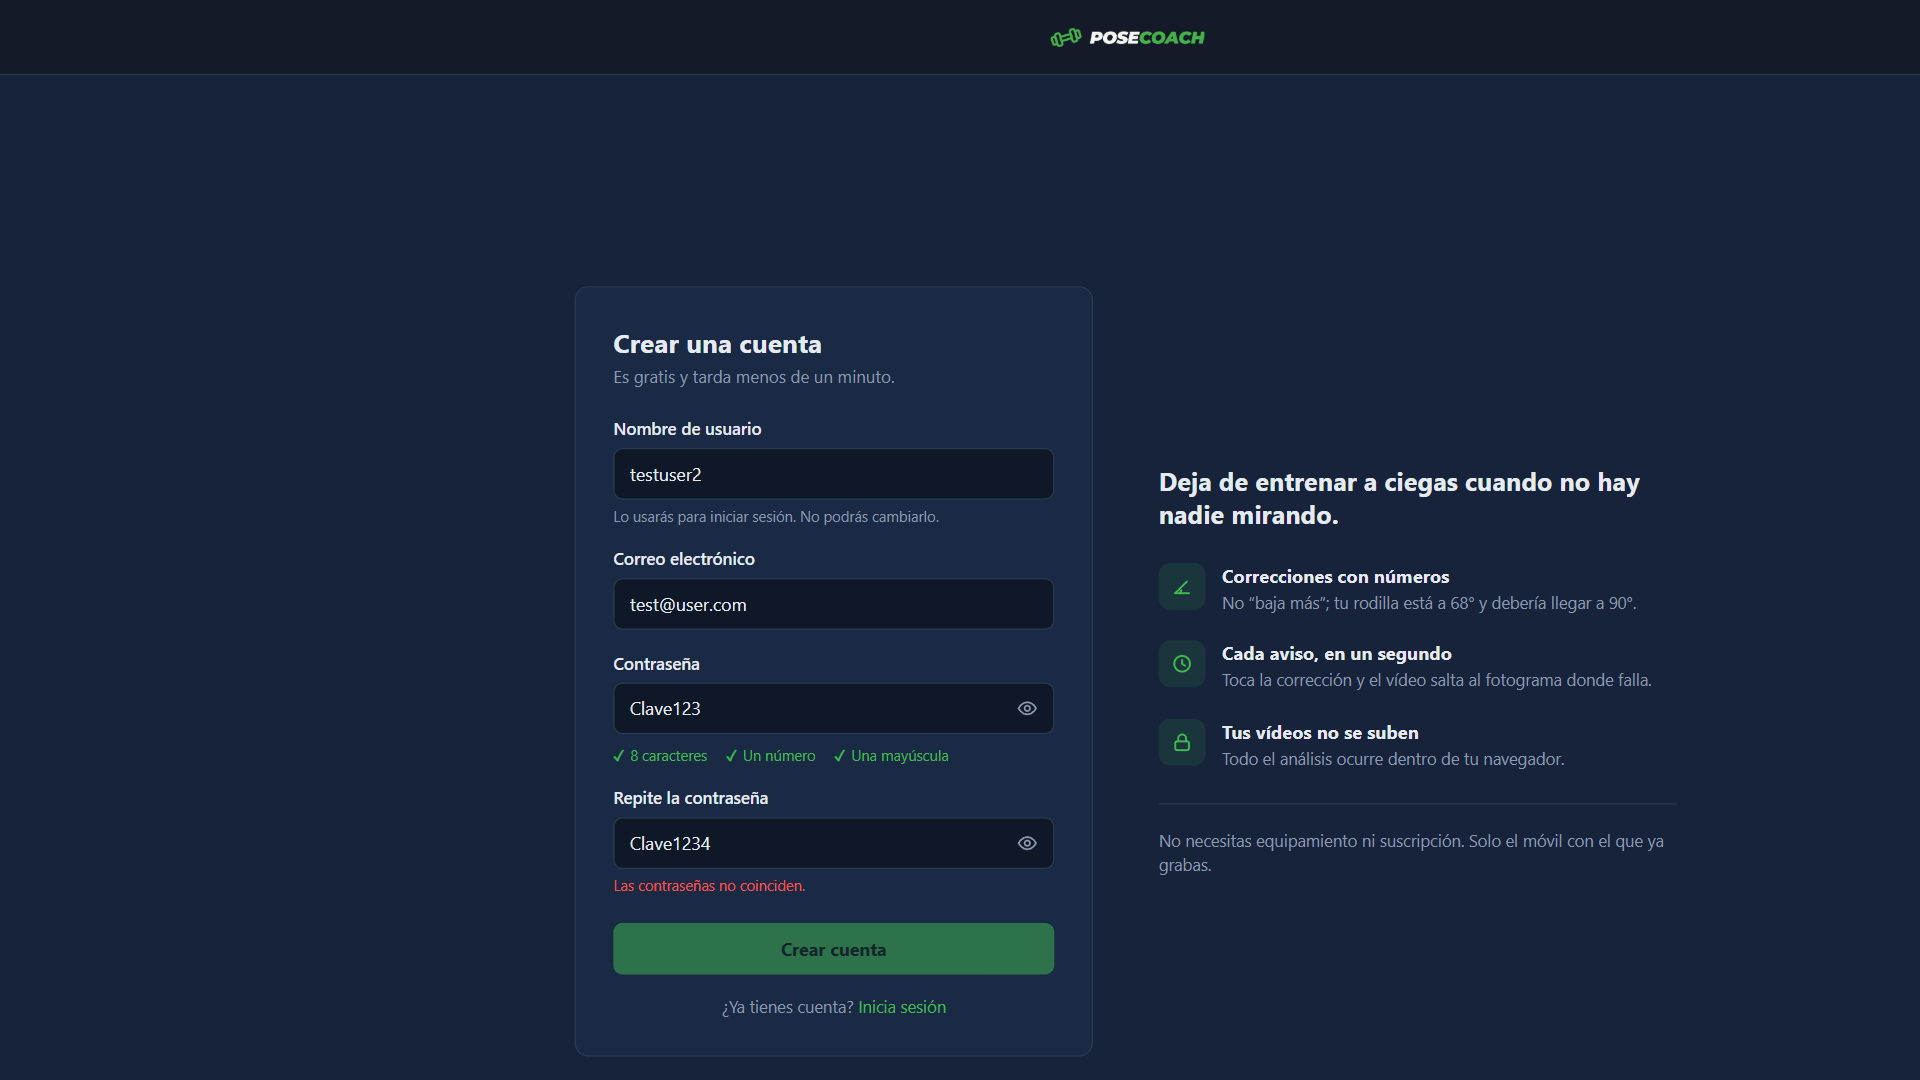
\includegraphics[width=\textwidth]{img/app-registro-validacion.png}
        \caption{Validación de la contraseña en tiempo real durante el registro:
        el botón permanece deshabilitado mientras no se cumplen todos los
        requisitos.}
        \label{fig:app-registro-validacion}
    \end{figure}

    \begin{figure}[htbp]
        \centering
        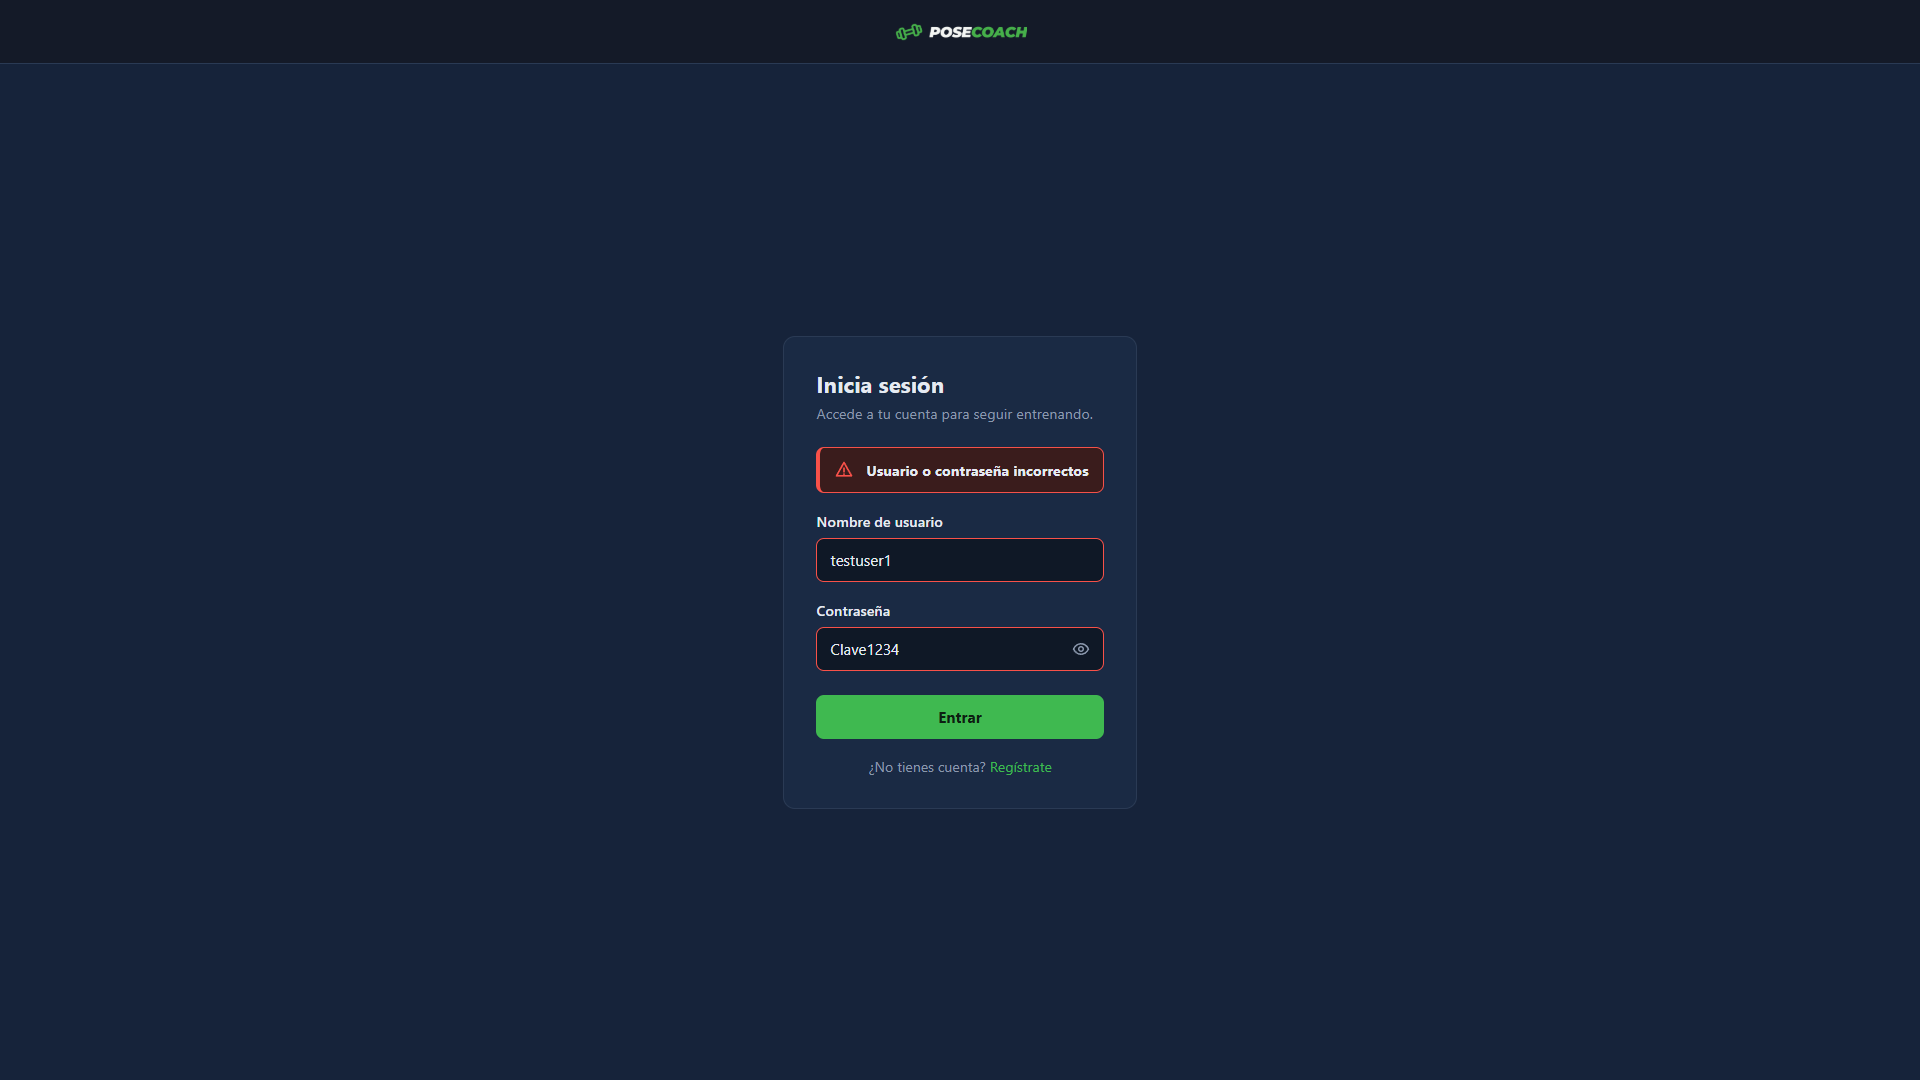
\includegraphics[width=0.7\textwidth]{img/app-login-error.png}
        \caption{Inicio de sesión con credenciales incorrectas: mensaje de error
        y resaltado de los campos afectados.}
        \label{fig:app-login-error}
    \end{figure}

    \begin{figure}[htbp]
        \centering
        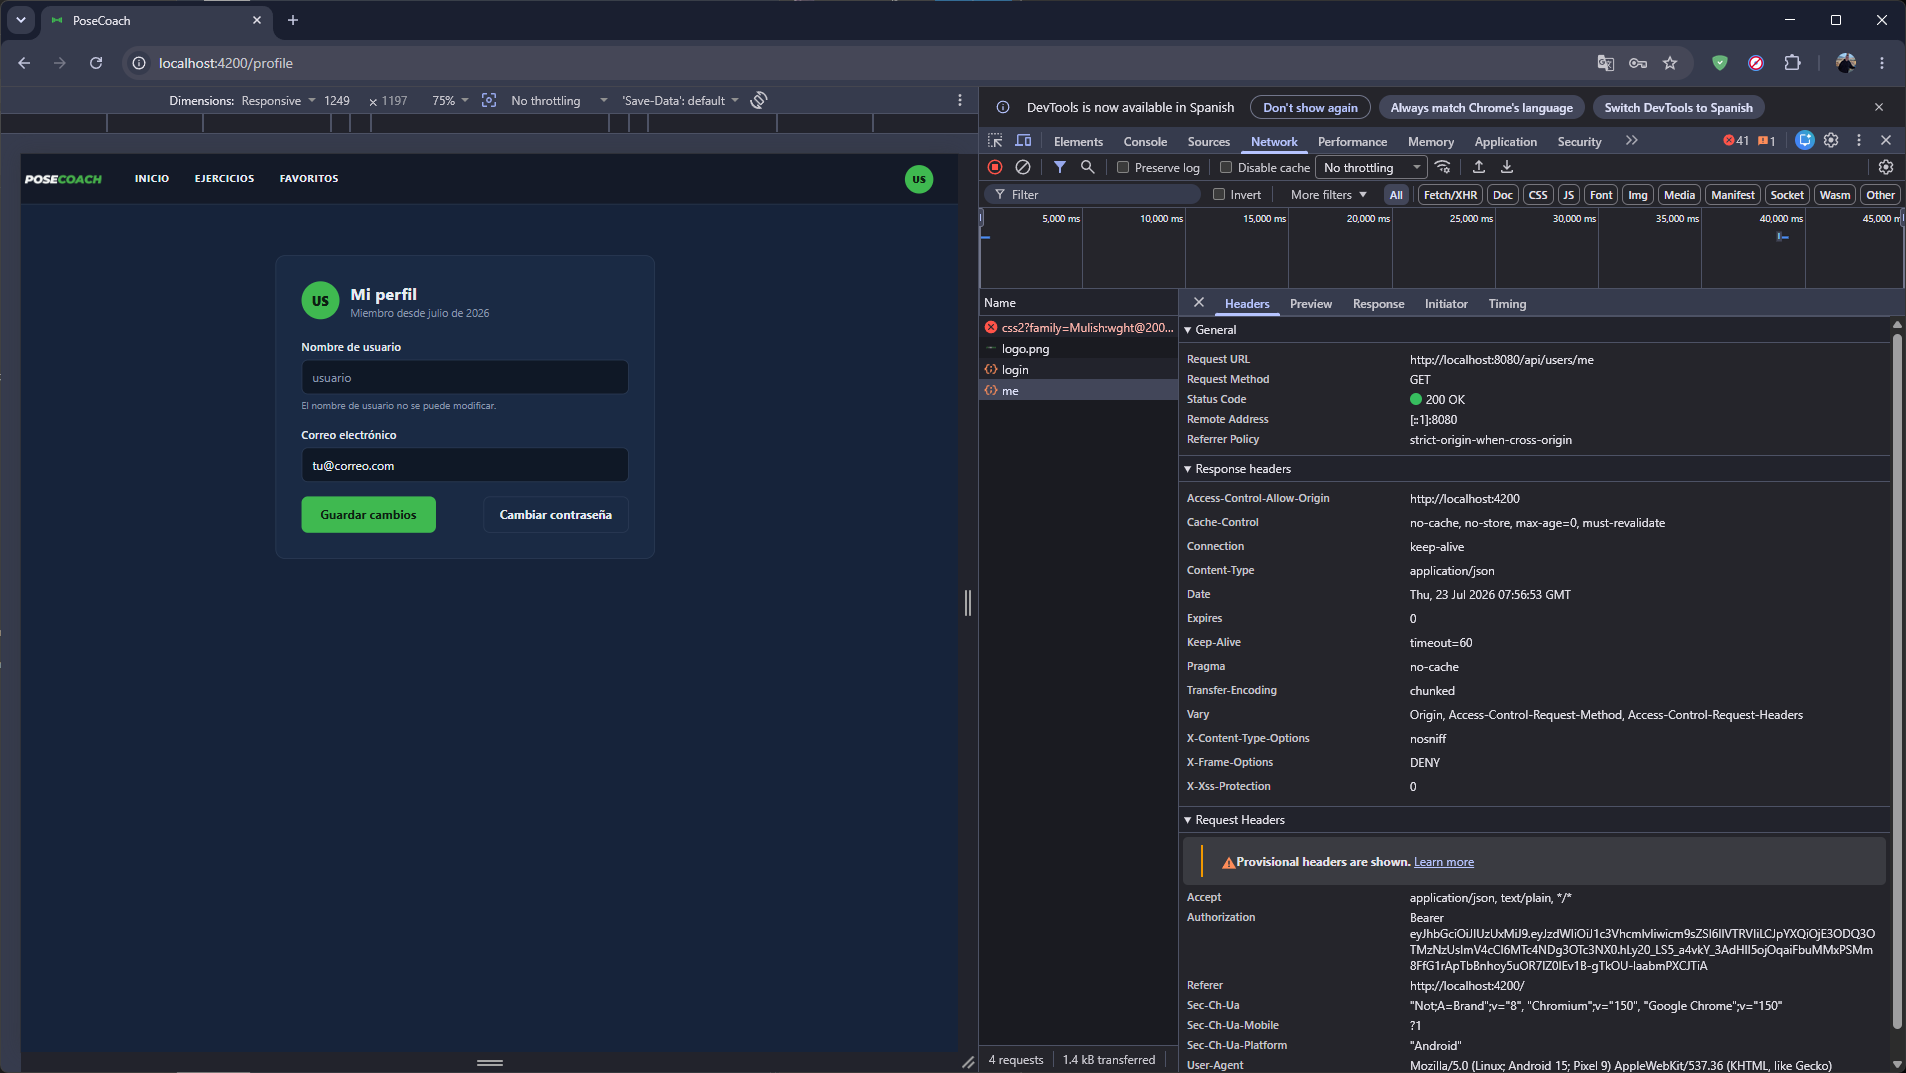
\includegraphics[width=\textwidth]{img/app-perfil-token.png}
        \caption{Petición al perfil del usuario: el interceptor adjunta
        automáticamente el token JWT en la cabecera \texttt{Authorization}.}
        \label{fig:app-perfil-token}
    \end{figure}

    \section{Pruebas del catálogo de ejercicios}

    Las operaciones del catálogo se han verificado con Postman, comprobando
    tanto los casos correctos como los de error. La
    Tabla~\ref{tab:pruebas-catalogo} recoge los casos ejecutados y el resultado
    esperado en cada uno.

    \begin{table}[htbp]
        \centering
        \begin{tabular}{p{7cm} l p{4cm}}
            \toprule
            \textbf{Caso} & \textbf{Código} & \textbf{Resultado esperado} \\
            \midrule
            Listado sin filtros                        & 200 & Diez ejercicios \\
            Búsqueda por nombre parcial                & 200 & Ejercicios coincidentes \\
            Búsqueda insensible a mayúsculas           & 200 & Mismo resultado \\
            Filtrado por dificultad                    & 200 & Ejercicios del nivel \\
            Filtrado por dos grupos musculares         & 200 & Ejercicios de alguno de ellos \\
            Filtrado combinado de grupo y dificultad   & 200 & Intersección de criterios \\
            Solicitud de una página concreta           & 200 & Página indicada \\
            Detalle de un ejercicio existente          & 200 & Descripción y consejos \\
            Valores admitidos por los filtros          & 200 & Grupos y dificultades \\
            Detalle de un identificador inexistente    & 404 & Mensaje de error \\
            Listado sin token de autenticación         & 401 & Acceso denegado \\
            Filtro con un valor no admitido            & 400 & Valores válidos \\
            \bottomrule
        \end{tabular}
        \caption{Casos de prueba de la API del catálogo de ejercicios.}
        \label{tab:pruebas-catalogo}
    \end{table}

    Dos de estos casos merecen comentario. El filtrado por dos grupos
    musculares confirma la semántica disyuntiva descrita en el capítulo de
    diseño: el resultado incluye ejercicios que trabajan uno solo de los grupos
    seleccionados, lo que no ocurriría con una interpretación conjuntiva. Y el
    listado sin token verifica que el catálogo es efectivamente privado, dado
    que la comprobación se realiza en la cadena de filtros del servidor y no
    depende de la interfaz.

    Las Figuras~\ref{fig:pruebas-catalogo-postman}
    y~\ref{fig:pruebas-catalogo-error} recogen la ejecución de ambos casos.

    \begin{figure}[htbp]
        \centering
        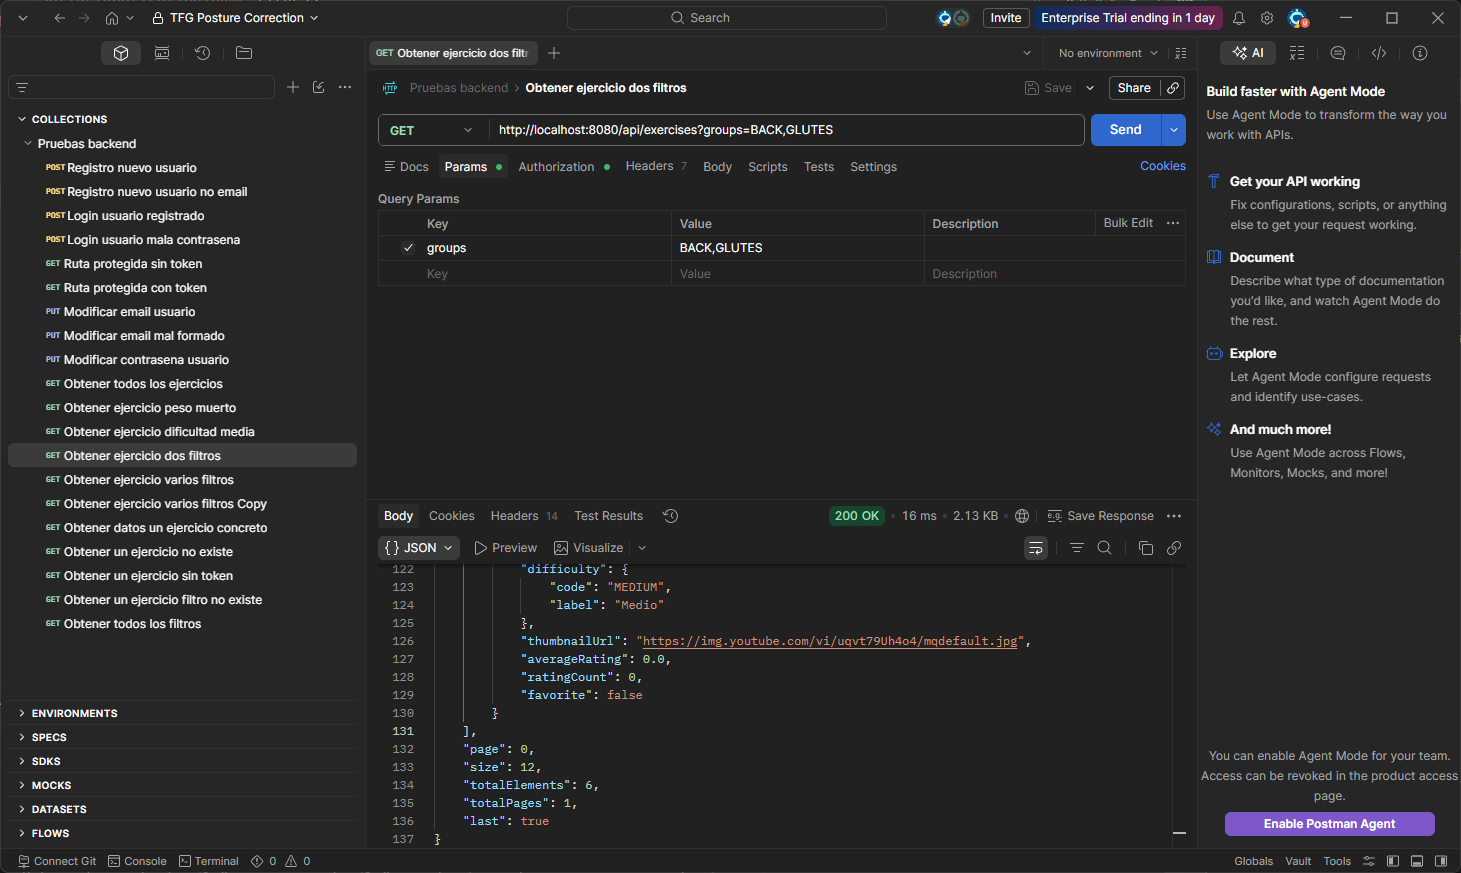
\includegraphics[width=0.9\textwidth]{img/pruebas-catalogo-postman.png}
        \caption{Filtrado por dos grupos musculares, con ejercicios que
        implican solo uno de ellos entre los resultados.}
        \label{fig:pruebas-catalogo-postman}
    \end{figure}

    \begin{figure}[htbp]
        \centering
        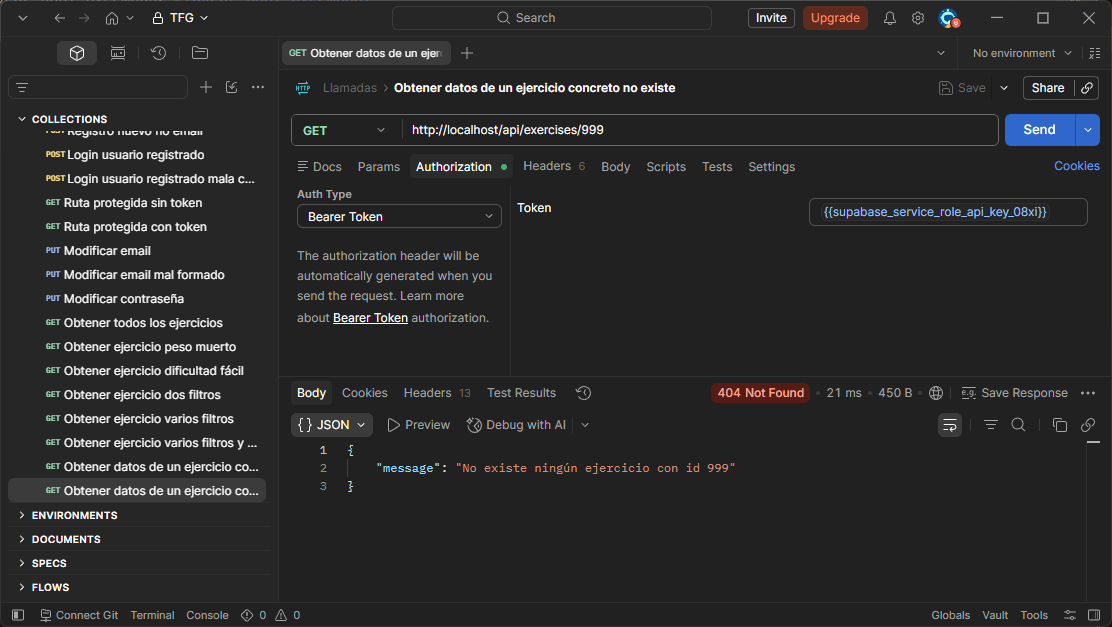
\includegraphics[width=0.9\textwidth]{img/pruebas-catalogo-error.png}
        \caption{Respuesta ante un valor no admitido en el parámetro de
        dificultad, con la relación de valores válidos.}
        \label{fig:pruebas-catalogo-error}
    \end{figure}

    \section{Pruebas del módulo de valoraciones y favoritos}

    La verificación de este módulo se organizó en cuatro frentes, atendiendo a
    la naturaleza de lo que se comprueba en cada caso: el comportamiento de los
    puntos de entrada de la API, el cumplimiento efectivo de las reglas de
    negocio y del control de acceso, el coste en accesos a la base de datos de
    las consultas de listado, y el recorrido completo de la interfaz. Los tres
    primeros se realizaron con Postman y consultas directas a MySQL; el último,
    de forma manual sobre la aplicación en ejecución.

    \subsection{Pruebas de la API}

    La Tabla~\ref{tab:pruebas-social-api} recoge los casos ejecutados sobre las
    rutas del módulo, junto con el código de estado y el resultado esperado en
    cada uno.

    \begin{table}[htbp]
        \centering
        \small
        \begin{tabular}{p{6.5cm} l p{4.5cm}}
            \toprule
            \textbf{Caso} & \textbf{Código} & \textbf{Resultado esperado} \\
            \midrule
            Registro de una valoración nueva              & 200 & Valoración creada \\
            Nueva valoración sobre el mismo ejercicio     & 200 & Mismo identificador, valores sustituidos \\
            Valoración con puntuación fuera del rango     & 400 & Mensaje con el rango admitido \\
            Valoración sin puntuación                     & 400 & Puntuación obligatoria \\
            Valoración sin comentario                     & 200 & Comentario nulo \\
            Comentario de más de 500 caracteres           & 400 & Mensaje de longitud máxima \\
            Valoración sobre un ejercicio inexistente     & 404 & Mensaje de error \\
            Eliminación de la valoración propia           & 204 & Sin contenido \\
            Eliminación repetida                          & 404 & No hay valoración que eliminar \\
            Resumen de valoraciones de un ejercicio       & 200 & Media, cinco niveles y valoración propia \\
            Listado de comentarios                        & 200 & Comentarios ajenos, paginados \\
            Marcado de un ejercicio como favorito         & 204 & Sin contenido \\
            Marcado repetido del mismo ejercicio          & 204 & Una única fila en la tabla \\
            Retirada de un favorito no marcado            & 204 & Sin contenido \\
            Listado de favoritos                          & 200 & Ordenados por fecha de marcado \\
            \bottomrule
        \end{tabular}
        \caption{Casos de prueba de la API de valoraciones y favoritos.}
        \label{tab:pruebas-social-api}
    \end{table}

    Cuatro de estos casos merecen comentario, por comprobar decisiones de
    diseño y no simplemente el funcionamiento de una operación.

    El segundo verifica la regla RN-01. Al emitir dos valoraciones consecutivas
    sobre el mismo ejercicio con puntuaciones distintas, la respuesta devuelve
    en ambos casos el mismo identificador
    (Figura~\ref{fig:postman-review-idempotente}), lo que evidencia que la
    segunda petición ha sustituido la fila existente en lugar de crear una
    nueva. Es la comprobación de que publicar y editar constituyen la misma
    operación.

    \begin{figure}[htbp]
        \centering
        \includegraphics[width=0.9\textwidth]{img/postman-review-idempotente.png}
        \caption{Dos valoraciones consecutivas sobre el mismo ejercicio: la
        respuesta conserva el identificador, confirmando la sustitución de la
        valoración anterior.}
        \label{fig:postman-review-idempotente}
    \end{figure}

    El caso de la valoración sin comentario comprueba la regla RN-03: la
    respuesta devuelve el comentario con valor nulo y la valoración computa en
    el resumen sin aparecer en el listado de comentarios. Como consecuencia, y
    tal como se aprecia en la Figura~\ref{fig:postman-summary}, el número de
    valoraciones de un ejercicio puede ser superior al de comentarios sin que
    ello suponga inconsistencia alguna. Esa misma figura permite verificar que
    la distribución devuelve siempre los cinco niveles de puntuación, incluidos
    aquellos que ninguna persona ha seleccionado.

    \begin{figure}[htbp]
        \centering
        \includegraphics[width=0.9\textwidth]{img/postman-summary.png}
        \caption{Resumen de valoraciones de un ejercicio: la distribución
        incluye los cinco niveles y el recuento supera al número de
        comentarios.}
        \label{fig:postman-summary}
    \end{figure}

    Los casos de marcado repetido y de retirada de un favorito no marcado
    verifican la idempotencia descrita en el capítulo de diseño: ambas
    peticiones se completan sin error y sin producir efecto adicional alguno,
    comprobándose en la base de datos que la tabla de favoritos no acumula
    filas duplicadas.

    Por último, la eliminación repetida de una valoración devuelve
    \texttt{404} mientras que la retirada repetida de un favorito devuelve
    \texttt{204}. Esta asimetría, deliberada y justificada en el capítulo de
    diseño, queda así documentada también en las pruebas.

    \subsection{Verificación de las reglas de negocio y del control de acceso}

    Las pruebas anteriores comprueban el comportamiento de la API cuando se
    utiliza conforme a lo previsto. Las de este apartado persiguen lo
    contrario: comprobar que las restricciones se sostienen ante intentos de
    eludirlas, incluyendo aquellos que no pasan por la propia aplicación. La
    Tabla~\ref{tab:pruebas-social-reglas} las recoge.

    \begin{table}[htbp]
        \centering
        \small
        \begin{tabular}{p{7cm} p{6cm}}
            \toprule
            \textbf{Prueba} & \textbf{Resultado esperado} \\
            \midrule
            Inserción manual en \texttt{reviews} de un par usuario--ejercicio ya existente & La base de datos rechaza la operación por violación de la restricción de unicidad \\
            Un usuario intenta eliminar la valoración de otro & 404, y la valoración ajena permanece intacta \\
            Petición sin cabecera de autorización & 401 \\
            Petición con un token alterado & 401 por firma no válida \\
            Cuerpo de la petición con un nombre de usuario ajeno & El campo se ignora y la valoración se registra a nombre del usuario del token \\
            \bottomrule
        \end{tabular}
        \caption{Pruebas de las reglas de negocio y del control de acceso.}
        \label{tab:pruebas-social-reglas}
    \end{table}

    La primera prueba se realiza deliberadamente al margen de la aplicación,
    mediante una sentencia \texttt{INSERT} ejecutada directamente sobre la base
    de datos (Figura~\ref{fig:duplicate-entry}). Su propósito no es comprobar
    la lógica del servicio, que nunca produciría esa situación, sino verificar
    que la regla RN-01 se sostiene aunque dicha lógica fallase o se ejecutase
    de forma concurrente. Es la diferencia entre una restricción implementada y
    una restricción garantizada.

    \begin{figure}[htbp]
        \centering
        \includegraphics[width=0.9\textwidth]{img/duplicate-entry.png}
        \caption{Intento de insertar una segunda valoración del mismo usuario
        sobre el mismo ejercicio: la restricción de unicidad de la tabla
        rechaza la operación.}
        \label{fig:duplicate-entry}
    \end{figure}

    La segunda es la prueba de autorización propiamente dicha, y conviene
    distinguirla de las pruebas de autenticación realizadas en el primer
    incremento. Allí se verificaba que un usuario no autenticado no accede al
    sistema; aquí se verifica que un usuario perfectamente autenticado no puede
    operar sobre datos ajenos. La Figura~\ref{fig:postman-review-ajena} recoge
    el intento de un usuario de eliminar la valoración de otro sobre el mismo
    ejercicio, junto con la consulta que confirma que la valoración original
    permanece almacenada. El código devuelto es \texttt{404} y no
    \texttt{403} porque, conforme al diseño descrito, la búsqueda se realiza
    siempre acotada al usuario autenticado: para el sistema no existe una
    valoración prohibida, sencillamente no existe ninguna valoración propia que
    eliminar.

    \begin{figure}[htbp]
        \centering
        \includegraphics[width=0.9\textwidth]{img/postman-review-ajena.png}
        \caption{Intento de eliminar la valoración de otro usuario: el servidor
        responde 404 y la valoración original permanece en la base de datos.}
        \label{fig:postman-review-ajena}
    \end{figure}

    \subsection{Verificación del coste de las consultas de listado}

    El listado del catálogo compone cada tarjeta con datos procedentes de tres
    tablas distintas, lo que lo expone al problema \textit{N+1} descrito en el
    capítulo anterior. Dado que este no se manifiesta como un error sino como
    una degradación progresiva del rendimiento, no puede detectarse
    comprobando la respuesta: es preciso observar las consultas que el sistema
    emite.

    Para ello se habilitó temporalmente el registro de las sentencias SQL
    generadas y se solicitó el listado completo del catálogo. La
    Figura~\ref{fig:log-sql-catalogo} recoge el resultado: el número de
    consultas permanece constante con independencia del número de ejercicios
    devueltos, con una única consulta agregada para las valoraciones y otra
    para los favoritos de toda la página, en lugar de una consulta por tarjeta.

    \begin{figure}[htbp]
        \centering
        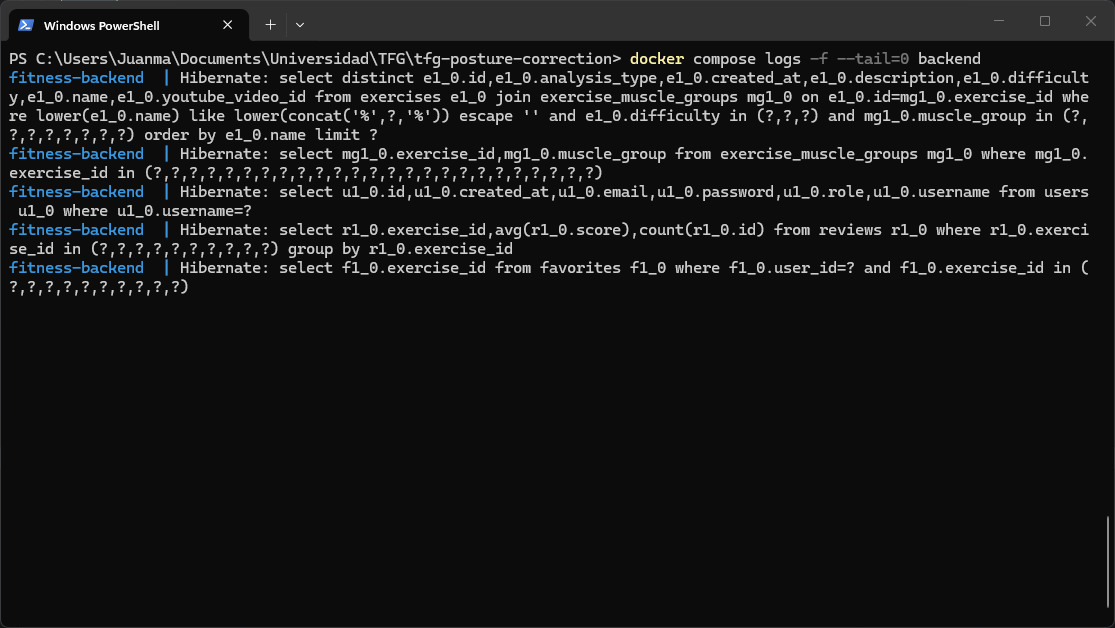
\includegraphics[width=0.95\textwidth]{img/log-sql-catalogo.png}
        \caption{Registro de las consultas SQL emitidas al solicitar el
        catálogo completo: el número de accesos no depende del número de
        ejercicios devueltos.}
        \label{fig:log-sql-catalogo}
    \end{figure}

    \subsection{Pruebas de integración de la interfaz}

    Por último se verificó el recorrido completo de la interfaz, con especial
    atención a los estados intermedios y a la coherencia entre vistas que
    muestran el mismo dato. La Tabla~\ref{tab:pruebas-social-ui} recoge los
    casos ejecutados.

    \begin{table}[htbp]
        \centering
        \small
        \begin{tabular}{p{6.5cm} p{6.5cm}}
            \toprule
            \textbf{Caso de prueba} & \textbf{Resultado esperado} \\
            \midrule
            Publicación de una valoración con comentario & Media, distribución, recuento y cabecera se actualizan simultáneamente \\
            Edición de una valoración publicada & El comentario se marca como editado y conserva su posición en el listado \\
            Valoración sin escribir comentario & Formulario bloqueado con las acciones accesibles y sin entrada en el listado \\
            Edición que vacía el texto del comentario & El comentario desaparece del listado y la puntuación sigue computando \\
            Eliminación de la valoración propia & Formulario reactivado y contadores a cero \\
            Dos usuarios valorando el mismo ejercicio & Cada uno ve su comentario destacado y el ajeno en el listado, sin duplicados \\
            Comentario con etiquetas HTML & El texto se muestra literalmente, sin interpretarse \\
            Ampliación del listado de comentarios & Los nuevos se añaden a los ya mostrados \\
            Marcado de un favorito y recarga de la página & El estado se mantiene \\
            Marcado desde el catálogo y consulta del detalle & Ambas vistas reflejan el mismo estado \\
            Retirada de un favorito desde la vista de favoritos & La tarjeta desaparece y el recuento disminuye \\
            Vista de favoritos con uno y con dos ejercicios & La barra de filtros aparece solo en el segundo caso \\
            Filtro sin coincidencias en favoritos & Mensaje específico, con la barra de filtros aún visible \\
            Acceso al detalle desde la vista de favoritos & El control de retroceso indica la vista de origen \\
            Acceso al detalle escribiendo la dirección & El control de retroceso adopta su valor por omisión \\
            Marcado de favorito desde el detalle & El vídeo no se reinicia y el retroceso funciona a la primera \\
            Dos usuarios con favoritos distintos & Cada uno consulta únicamente los suyos \\
            \bottomrule
        \end{tabular}
        \caption{Casos de prueba de la interfaz del módulo de valoraciones y
        favoritos.}
        \label{tab:pruebas-social-ui}
    \end{table}

    Todos los casos se completaron con el resultado esperado, si bien dos de
    ellos lo hicieron únicamente tras corregir sendos defectos detectados
    durante su ejecución, descritos en el capítulo anterior: la
    inaccesibilidad de las acciones de edición y eliminación al valorar sin
    comentar, y la recarga del marco flotante del vídeo al modificar la
    condición de favorito.

    Merece destacarse el caso del comentario con etiquetas HTML
    (Figura~\ref{fig:app-comentario-escapado}), que verifica la protección
    frente a la inyección de código en contenido redactado por usuarios, y el
    de la edición que vacía el texto, que comprueba de extremo a extremo la
    normalización descrita en la implementación: el comentario desaparece del
    listado mientras la puntuación permanece en la distribución.

    \begin{figure}[htbp]
        \centering
        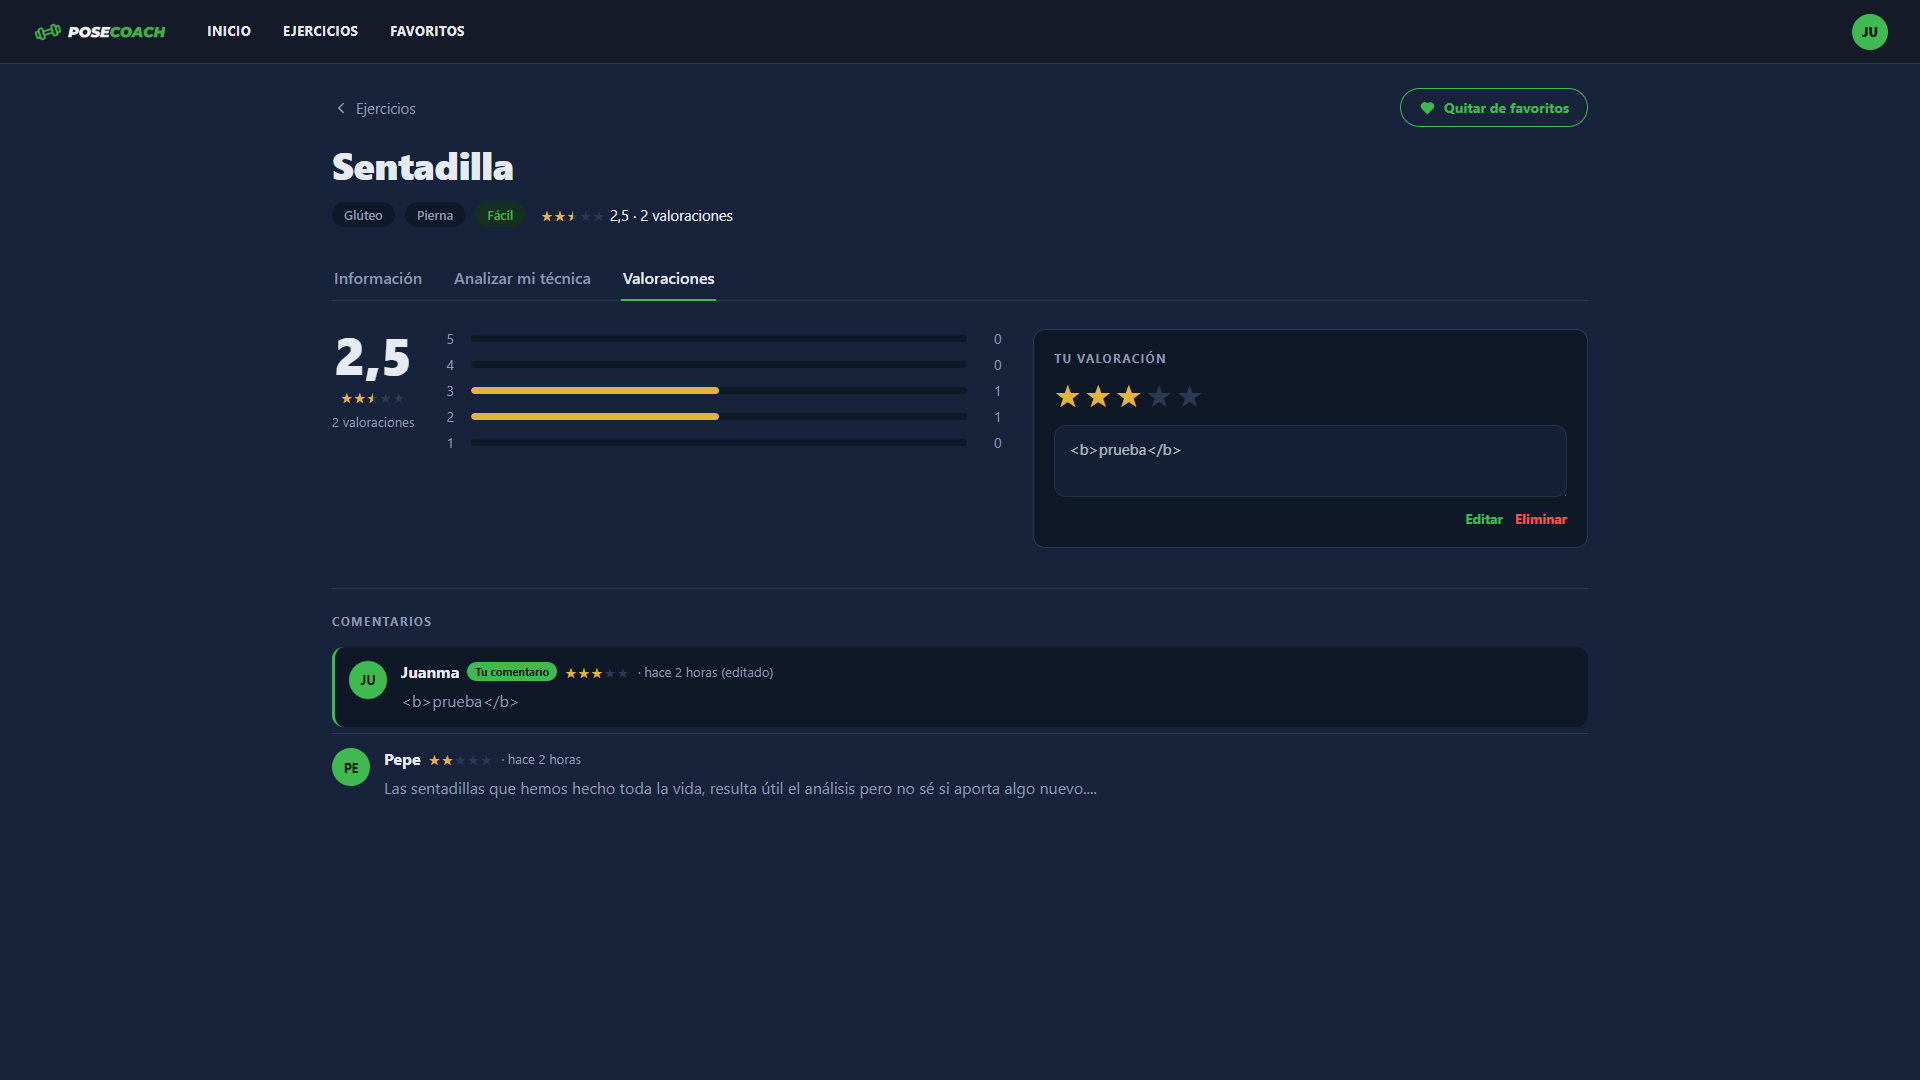
\includegraphics[width=0.9\textwidth]{img/app-comentario-escapado.png}
        \caption{Comentario que incluye etiquetas HTML: el contenido se
        representa como texto literal y no llega a interpretarse.}
        \label{fig:app-comentario-escapado}
    \end{figure}

    Las Figuras~\ref{fig:app-valoraciones}, \ref{fig:app-valoraciones-publicada}
    y~\ref{fig:app-favoritos} recogen el aspecto final de las pantallas
    implementadas.

    \begin{figure}[htbp]
        \centering
        \includegraphics[width=\textwidth]{img/app-valoraciones.png}
        \caption{Pestaña de valoraciones de un ejercicio, con la distribución
        de puntuaciones, el formulario de valoración y el listado de
        comentarios.}
        \label{fig:app-valoraciones}
    \end{figure}

    \begin{figure}[htbp]
        \centering
        \includegraphics[width=\textwidth]{img/app-valoraciones-publicada.png}
        \caption{Pestaña de valoraciones con una valoración ya publicada:
        formulario bloqueado con las acciones de edición y eliminación, y
        comentario propio destacado.}
        \label{fig:app-valoraciones-publicada}
    \end{figure}

    \begin{figure}[htbp]
        \centering
        \includegraphics[width=\textwidth]{img/app-favoritos.png}
        \caption{Vista de ejercicios favoritos, con la barra de filtros
        heredada del catálogo.}
        \label{fig:app-favoritos}
    \end{figure}


    \section{Resultados}


% ─────────────────────── Capítulo 8 ──────────────────────────────────


    \chapter{Conclusiones y trabajo futuro}
    \label{cap:conclusiones}


    \section{Conclusiones}

    \section{Dificultades encontradas}

    El desarrollo se ha visto jalonado por un conjunto de incidencias cuya
    resolución ha aportado tanto al resultado como la propia implementación.
    Se recogen aquí las más representativas, agrupadas según su naturaleza.

    \subsection{Comportamientos por omisión de los marcos de trabajo}

    Varias incidencias tuvieron su origen en decisiones que los marcos de
    trabajo adoptan por defecto y que resultan inadecuadas para una API REST.
    La incorporación de Spring Security dejó inaccesible el registro de
    usuarios, al proteger todos los puntos de entrada, y las peticiones de
    escritura comenzaron a rechazarse con \texttt{403 Forbidden} por una
    protección contra falsificación de peticiones concebida para formularios
    con sesión, ajena por completo a un servidor sin estado. En ambos casos el
    síntoma resultaba desconcertante hasta comprender qué estaba activo sin
    haberlo solicitado.

    Un caso análogo se dio con la carga de asociaciones en JPA. La estrategia
    diferida, adecuada como norma general, provocaba un error al construir los
    objetos de transferencia fuera de la transacción; corregirlo mediante carga
    anticipada introdujo a su vez el problema \textit{N+1}, con una consulta
    adicional por cada elemento del listado. La solución definitiva no consistió
    en elegir una de las dos estrategias, sino en aplicar a cada colección la
    que corresponde a su uso real y agrupar las consultas resultantes.

    \subsection{Efectos colaterales del modelo reactivo del cliente}

    El modelo de reactividad basado en señales detecta los cambios comparando
    referencias, lo que obliga a sustituir los objetos en lugar de modificarlos.
    Esta exigencia, razonable en sí misma, produjo un efecto inesperado al
    incorporar el marcado de favoritos a la vista de detalle: la sustitución del
    objeto propagaba un recálculo hasta la dirección del vídeo embebido,
    provocando la recarga del marco flotante y, con ella, una entrada adicional
    en el historial del navegador que obligaba a pulsar dos veces el control de
    retroceso. El síntoma se manifestaba en la navegación, tres pasos por
    delante de su causa, y su diagnóstico ilustra la dificultad de depurar
    sistemas en los que los cambios se propagan de forma implícita.

    \subsection{Defectos detectables solo en el recorrido completo}

    La verificación de los puntos de entrada de la API por separado no basta
    para garantizar que la aplicación sea utilizable. El caso más ilustrativo
    fue el de un usuario que puntuase un ejercicio sin escribir comentario: la
    API respondía correctamente, pero la interfaz situaba las acciones de
    edición y eliminación junto a un comentario que en ese caso no existía,
    dejándolo sin ninguna forma de modificar o retirar su valoración. Ninguna
    prueba de la API habría revelado el problema, que solo apareció al recorrer
    la aplicación como lo haría un usuario.

    \subsection{Coherencia del código a lo largo del tiempo}

    El desarrollo incremental tiende a producir divergencias entre lo escrito en
    momentos distintos: dos criterios simultáneos de organización en paquetes,
    dos estilos de inyección de dependencias, dos formatos de respuesta de
    error, o una misma regla de estilo repetida en varias hojas. Ninguna
    constituye un error funcional, y precisamente por ello resulta sencillo
    acumularlas. La estrategia adoptada fue registrarlas como tareas específicas
    en el momento de detectarlas y resolverlas de forma agrupada al cierre de
    cada incremento, evitando tanto interrumpir el trabajo en curso como
    olvidarlas.

    \subsection{Herramientas}

    Por último, la carga inicial del \textit{backlog} en Jira mediante
    importación de ficheros resultó infructuosa tras varios intentos, por lo que
    las tareas se dieron de alta manualmente. La incidencia, de escasa entidad
    técnica, ilustra un riesgo habitual en la gestión de proyectos: el tiempo
    invertido en automatizar una tarea puntual puede superar con holgura al de
    ejecutarla a mano.


    \section{Líneas de trabajo futuro}

    \subsection{Seguridad y despliegue}

    El sistema de autenticación implementado cumple su cometido en el entorno
    de desarrollo, pero un despliegue real exigiría abordar tres cuestiones.

    La primera es el uso de un canal cifrado. Durante el desarrollo la
    comunicación se realiza sobre HTTP, de modo que el token viaja en claro; y
    dado que un token JWT va firmado pero no cifrado, cualquiera que lo
    interceptase podría leer su contenido y reutilizarlo hasta su caducidad.
    Esta circunstancia es precisamente la razón por la que el token no
    incorpora ningún dato sensible más allá del nombre de usuario y su rol.

    La segunda es la ausencia de un mecanismo de revocación. Al no mantenerse
    ninguna sesión en el servidor, cerrar sesión se limita a eliminar el token
    del cliente, mientras que una copia sustraída seguiría siendo válida hasta
    expirar. La solución habitual combina una caducidad breve con un segundo
    token de renovación, planteamiento que excede el alcance de este trabajo.

    La tercera afecta a la gestión de credenciales. La clave de firma se ha
    extraído a una variable de entorno con un valor de desarrollo por defecto,
    de manera que no figure en el repositorio. Conviene subrayar, no obstante,
    que un secreto que haya llegado a registrarse en el historial de un sistema
    de control de versiones permanece accesible en él aunque se elimine del
    fichero, por lo que un despliegue real debe emplear una credencial nueva y
    no la utilizada durante el desarrollo.

    A ello se añade que el registro de usuarios no verifica la titularidad del
    correo electrónico. La regla que limita a una la valoración por usuario y
    ejercicio acota el efecto de una eventual creación masiva de cuentas sobre
    las valoraciones, pero no lo elimina.

    \subsection{Evolución del módulo de valoraciones y favoritos}

    Varias decisiones de este incremento resultan adecuadas al volumen de datos
    previsto pero dejarían de serlo con un uso intensivo. El filtrado de la
    vista de favoritos se resuelve en el navegador sobre la lista ya
    descargada, lo que ofrece una respuesta inmediata mientras el número de
    ejercicios guardados sea reducido; una lista extensa exigiría trasladar el
    filtrado al servidor, reutilizando los parámetros que ya admite el
    catálogo. Del mismo modo, la vista de favoritos no incorpora paginación,
    prescindible con un catálogo de diez ejercicios pero necesaria si este
    creciera.

    Las marcas temporales se almacenan sin información de zona horaria, lo que
    resulta correcto mientras servidor y usuarios comparten la misma, pero
    impide un despliegue en varias regiones. Sustituirlas por un tipo que
    incorpore la referencia temporal absoluta resolvería la limitación y
    permitiría al cliente adaptar la representación a la zona de cada usuario.

    Por último, el módulo admite extensiones funcionales que no se han abordado
    por quedar fuera de los requisitos: la posibilidad de responder a un
    comentario, la moderación de contenido inadecuado o la ordenación del
    catálogo por valoración media, para la que el modelo de datos actual ya
    dispone de la información necesaria.

    \subsection{Deuda técnica identificada}

    El seguimiento del proyecto incorporó desde el primer incremento un
    registro explícito de mejoras técnicas detectadas durante el desarrollo
    pero no abordadas en el momento, con el fin de evitar tanto la
    interrupción constante del trabajo en curso como el olvido de las
    incidencias. La mayor parte se resolvió al cierre de cada incremento, según
    se describe en el Capítulo~\ref{cap:implementacion}; el resto permanece
    documentado y razonado.

    Entre lo pendiente destaca la extracción de los campos de auditoría de las
    entidades a una clase base común, que eliminaría la repetición de los
    métodos de asignación de marcas temporales en las cuatro entidades del
    modelo. Se pospuso por afectar simultáneamente a todas ellas en un momento
    del calendario en que la prioridad era completar la funcionalidad prevista.

    Otras decisiones se descartaron de forma razonada por resultar su coste
    superior al beneficio con el volumen de datos previsto: incorporar el
    identificador del usuario al token para evitar una consulta por petición,
    lo que acoplaría el token al modelo de datos, y reforzar el mecanismo de
    retroceso del navegador frente a interacciones del usuario con el
    reproductor de vídeo embebido. Documentar estos descartes junto a su
    justificación permite distinguir la deuda técnica asumida de forma
    deliberada de aquella que responde a un descuido.


% ─────────────────────── Apéndices ───────────────────────────────────
    \begin{umaappendices}

        \umaappendix{Seguimiento del proyecto en Jira}
% Capturas del tablero, backlog y gráficos de sprint/burndown.

        \umaappendix{Manual de instalación y despliegue}
% Requisitos previos, docker-compose, arranque de los servicios.

        \umaappendix{Manual de usuario}
% Registro, navegación por el catálogo, uso del análisis postural.

    \end{umaappendices}

% ======================================================================
%  A continuación, en main.tex, va \backmatter y \printbibliography
% ======================================================================
%────────────────────── Back cover and bibliography ────────────────────
    \backmatter
    \printbibliography[title={Bibliografía}]
    \cleardoublepage
    \MakeUMABackCover

\end{document}
% ======================================================================
